\documentclass[fancy,estyle,twoside,a4paper]{ethesis}

%The following two packages are required to have awesome font qualities!
\usepackage{ae,aecompl} %,placeins


% ========== Mathematics 

\usepackage{amsmath,amssymb,amstext,amsthm}
\usepackage{blkarray}
\numberwithin{equation}{section}
\usepackage{mathtools}

\usepackage{empheq}
\usepackage[most]{tcolorbox}

\usepackage{hyperref}

\usepackage[round]{natbib}

% ========== Color

\usepackage{color,soul,bm}
\usepackage{colortbl}
\usepackage[normalem]{ulem} %to have nice underlining, for exmaple try \uwave{blahblah}
\usepackage{graphicx}

\usepackage{fancyhdr}
\usepackage{lettrine} %Typeset dropped capitals

% ========== Algorithm

%\usepackage[chapter, ruled]{algorithm}
\usepackage[ruled,vlined,linesnumbered,boxed]{algorithm2e}
\usepackage{color}

\usepackage{bibentry}
\nobibliography*

% ========== Figures
  
\usepackage{multirow}
\usepackage[footnotesize,bf,hang]{caption,subfigure}

%\captionsetup[algorithm]{font=small}
\usepackage{booktabs} %Publication quality tables in LaTeX

%\usepackage{mathrsfs} %cool font, see http://zelmanov.ptep-online.com/ctan/symbols-a4.pdf
%\usepackage[table]{xcolor}
\usepackage[titletoc,toc,page]{appendix}

%\usepackage[backref,bookmarks=true, breaklinks]{hyperref} % clickable back-references from the bibliography list to citing sections
\usepackage{tcolorbox}
\tcbuselibrary{theorems}
\usepackage{soul}
\usepackage{enumitem}
\usepackage{verbatim}
\usepackage{multirow}
\usepackage{tikz} % drawing tools in latex
%\usepackage[paperwidth=25cm,paperheight=22cm,left=1cm,top=1cm]{geometry}
\usetikzlibrary{mindmap,shadows}

\RequirePackage{natbib}
\usepackage{color, colortbl}
\definecolor{Gray}{gray}{0.9}
\usepackage{placeins}


\usepackage[utf8]{inputenc}
\inputencoding{latin1}
\usepackage[T1]{fontenc}



\newlist{mylist}{enumerate}{5}  % Specify 5 Levels as clone of enumerate
\setlist[mylist,1]{label={\arabic*.}}  % Roman uppercase numbers I.
\setlist[mylist,2]{label={\Alph*.}}   % Latin uppercase letters A.
\setlist[mylist,3]{label={\arabic*.}} % arabic numbers 1.
\setlist[mylist,4]{label={\alph*.}}   % Latin lowercase letters a.
\setlist[mylist,5]{label={(\roman*)}} % roman lowercase letters in ()

% Information boxes
\newcommand*{\info}[4][16.3]{%
  \node [ annotation, #3, scale=0.65, text width = #1em,
          inner sep = 2mm ] at (#2) {%
  \list{$\bullet$}{\topsep=0pt\itemsep=0pt\parsep=0pt
    \parskip=0pt\labelwidth=8pt\leftmargin=8pt
    \itemindent=0pt\labelsep=2pt}%
    #4
  \endlist
  };	
}

\usepackage[makeroom]{cancel}


\hypersetup{colorlinks={true},
            linkcolor={blue},
            anchorcolor={blue},
            citecolor={blue},
            filecolor={blue},
            urlcolor={blue},
            menucolor={blue},
            }

	\newcommand{\gDisplayTitle}{}
	\newcommand{\gDisplayPreamble}{}
	\newcommand{\gDisplayTableOfContents}{}
	\newcommand{\gDisplayIntroduction}{}
	\newcommand{\gDisplayBackground}{}       

	\newcommand{\gDisplaySearch}{}
        \newcommand{\gDisplayPegSocket}{}
	\newcommand{\gDisplayMLMF}{}
	\newcommand{\gDisplayConclusions}{}
	\newcommand{\gDisplayAppendix}{}
	\newcommand{\gDisplayBibliography}{}

\newcommand{\tagMainFile}

\DeclareMathOperator{\E}{\displaystyle \mathop{\mathbb{E}}}

\DeclareMathOperator*{\argminA}{arg\,min}   % rbp
\DeclareMathOperator*{\argmaxA}{arg\,max} % thin space, limits underneath in displays

\DeclareMathOperator{\Unn}{\dot{x}}

\DeclareMathOperator{\policy}{\pi_{\boldsymbol{\theta}}}
\DeclareMathOperator{\BigO}{\mathcal{O}}
\newcommand{\X}{x}
\newcommand{\B}{b}
\newcommand{\U}{\dot{x}}

\newcommand{\Ui}{\dot{x}^{[i]}}
\newcommand{\Bi}{b^{[i]}}
\newcommand{\Xm}{x^{[m]}}

\newcommand{\ThAs}{\boldsymbol{\theta}^*_a}
\newcommand{\ThOs}{\boldsymbol{\theta}^*_o}

\newcommand{\ThA}{\boldsymbol{\theta}_a}
\newcommand{\ThO}{\boldsymbol{\theta}_o}
\newcommand{\BAlph}{\boldsymbol{\alpha}_{\mathbf{0:t}}}
\newcommand{\Alpha}{\alpha_{0:t}}
\newcommand{\BPsi}{\boldsymbol{\Psi_{0:t}}}

\newcommand{\invSigK}{\boldsymbol{\Sigma}^{[k]^{-1}}}
\newcommand{\SigK}{\boldsymbol{\Sigma}^{[k]}}
\newcommand{\Sig}[1]{\boldsymbol{\Sigma}^{[#1]}}
\newcommand{\Mu}[1]{\boldsymbol{\mu}^{[#1]}}
\newcommand{\MuK}{\boldsymbol{\mu}^{[k]}}
\newcommand{\Muk}{\boldsymbol{\mu}_k}
\newcommand{\Bx}{\mathbf{x}}
\newcommand{\Qpx}{Q^{\pi_{\Param'}}(\mathbf{x}^{[j]})}


\newcommand{\xb}{\dot{x}|b}

\newcommand{\piK}{w^{[k]}}
\newcommand{\Param}{\boldsymbol{\theta}}

\newcommand{\V}{\ensuremath{\mathcal{V}}}
\newcommand{\varOne}{\ensuremath{\sigma_{x}^{2}}}
\newcommand{\varTwo}{\ensuremath{\sigma_{m}^{2}}}
\newcommand{\stdOne}{\ensuremath{\sigma_{x}}}
\newcommand{\stdTwo}{\ensuremath{\sigma_{m}}}
\newcommand\independent{\protect\mathpalette{\protect\independenT}{\perp}}\def\independenT#1#2{\mathrel{\rlap{$#1#2$}\mkern2mu{#1#2}}}
\newcommand{\dependent}{\rotatebox[origin=c]{180}{$\independent$}}
%\newcommand{\BigO}[1]{\ensuremath{\operatorname{O}\bigl(#1\bigr)}}

\newcommand\Ccancel[2][black]{\renewcommand\CancelColor{\color{#1}}\cancel{#2}}

\newsavebox{\fmbox}
\newenvironment{fmpage}[1]
{\begin{lrbox}{\fmbox}\begin{minipage}{#1}}
{\end{minipage}\end{lrbox}\fbox{\usebox{\fmbox}}}

\DeclareMathOperator{\Tr}{Tr}
\DeclareCaptionLabelFormat{adja-page}{\hrulefill\\#1 #2 \emph{(previous page)}}

\definecolor{dark-green}{RGB}{0,100,0}
\definecolor{dark-blue}{RGB}{28,107,145}


\usepackage{color}

\newcommand*{\mathcolor}{}
\def\mathcolor#1#{\mathcoloraux{#1}}
\newcommand*{\mathcoloraux}[3]{%
  \protect\leavevmode
  \begingroup
    \color#1{#2}#3%
  \endgroup
}



\usepackage{tikz}
\usetikzlibrary{decorations.pathreplacing,calc}
\newcommand{\tikzmark}[1]{\tikz[overlay,remember picture] \node (#1) {};}

\newcommand*{\AddNote}[4]{%
    \begin{tikzpicture}[overlay, remember picture]
        \draw [decoration={brace,amplitude=0.5em},decorate,ultra thick,red]
            ($(#3)!(#1.north)!($(#3)-(0,1)$)$) --  
            ($(#3)!(#2.south)!($(#3)-(0,1)$)$)
                node [align=center, text width=2.5cm, pos=0.5, anchor=west] {#4};
    \end{tikzpicture}
}%


\let\oldnl\nl% Store \nl in \oldnl
\newcommand{\nonl}{\renewcommand{\nl}{\let\nl\oldnl}}% Remove line number for one line



\graphicspath{{ch1-Introduction/Figures/}}

\begin{document}

%%%%%%%%%%%%%%%%%%%%%%%
% Math Macros

\newcommand{\ud}{\,\mathrm{d}}

\def\mat#1{\mathchoice{\mbox{\boldmath$\displaystyle#1$}}
{\mbox{\boldmath$\textstyle#1$}}
{\mbox{\boldmath$\scriptstyle#1$}}
{\mbox{\boldmath$\scriptscriptstyle#1$}}}

\newcommand{\acos}{\mathrm{acos}}

% \widebar math accent
\newlength{\widebarargwidth}
\newlength{\widebarargheight}
\DeclareRobustCommand{\widebar}[1]{%
	\settowidth{\widebarargwidth}{#1}%
	\settoheight{\widebarargheight}{#1}%
	\addtolength{\widebarargheight}{0.3ex}
	\makebox[0pt][l]{\hspace{0.15\widebarargwidth}%
		\rule[\widebarargheight]{0.7\widebarargwidth}{0.1ex}}%
	{#1}}


%%%%%%%%%%%%%%%%%%%%%%%
% Misc Macros

%\newcounter{deft}
%\renewcommand{\thedeft}{Theorem \thechapter.\arabic{deft}}
%\newenvironment{theorem}[1]
%{\refstepcounter{deft} \begin{trivlist} \item[\hskip \labelsep {\bfseries \thedeft}] {\em #1}}
%{\end{trivlist}}
%
%
%\newcounter{defd}
%\renewcommand{\thedefd}{Definition \thechapter.\arabic{defd}}
%\newenvironment{definition}[1]
%{\refstepcounter{defd} \begin{trivlist} \item[\hskip \labelsep {\bfseries \thedefd}] {\em #1}}
%{\end{trivlist}}

\newenvironment{challenge}[2][Challenge:]
{\begin{trivlist}
\item \vskip \baselineskip \noindent $\square$
\item \textbf{\textsc{#1}} {#2}
\item \hfill $\blacksquare$
\end{trivlist}
}


\newcommand{\tbc}{\highlight{[To be completed...]}}
\newcommand{\keyword}[1]{\textsc{\textbf{Keyword(s): #1}}}
\newcommand{\tbr}[1]{\highlight{[To be rewritten: }\emph{#1}\highlight{]}}
\newcommand{\highlight}[1]{\textsf{#1}}
\newcommand{\bhighlight}[1]{\textbf{\textsf{#1}}}
\newcommand{\khighlight}[1]{\textsc{#1}}
\newcommand{\bfid}[1]{\textbf{#1}}

\renewcommand{\paragraph}[1]{\vspace{0.4cm}\noindent\bhighlight{#1}\vspace{0.15cm}}

\newcommand{\subsubsubsection}{\paragraph}

\newcommand{\mylineskip}{\vspace{0.4cm}}

%\newcommand{\comment}[1]{}
%\newcommand{\commentary}[1]{\bhighlight{[Comment:} \highlight{#1}\bhighlight{]}}

\newcommand{\FigureFrom}[1]{{\it (Adapted from \protect\citeA{#1})}}
\newcommand{\FiguresFrom}[1]{{\it (Adapted from \protect\citeA{#1})}}
\newcommand{\FigureNoFrom}[2]{{\it (Figure} \bfid{#1)} {\it is adapted from \protect\citeA{#2})}}
%%%% debut macro %%%%

%%%%%%%%%%%%%%%%%%%%%%%%%%%%%%%%%%%%%%%%%%%%%%%%%%%%%%%%%%%%%%%%%%%%%%
%% The \todo command
\newcounter{nbdrafts}
\setcounter{nbdrafts}{0}
\makeatletter
\newcommand{\checknbdrafts}{
\ifnum \thenbdrafts > 0
\@latex@warning@no@line{**********************************************************************}
\@latex@warning@no@line{* The document contains \thenbdrafts \space draft note(s)}
\@latex@warning@no@line{**********************************************************************}
\fi}
\newcommand{\todo}[1]{\addtocounter{nbdrafts}{1}{\color{red} #1}}
\makeatother
%%%%%%%%%%%%%%%%%%%%%%%%%%%%%%%%%%%%%%%%%%%%%%%%%%%%%%%%%%%%%%%%%%%%%%
\def\argmax{\operatornamewithlimits{argmax}}
\def\argmin{\operatornamewithlimits{argmin}}

%\newcommand{\corrected}[1]{{\color{red} \uwave{#1}}}
\definecolor{myCorrectionColor}{RGB}{34,139,34}
\newcommand{\corrected}[1]{{\color{myCorrectionColor} #1}}


\newcommand{\fvspace}{-1.0cm}

\newcommand{\eqspacedab}{a)\hspace{0.45\textwidth}b)}
\newcommand{\eqspacedabc}{a)\hspace{0.30\textwidth}b)\hspace{0.30\textwidth}c)}
\newcommand{\eqspacedabcd}{a)\hspace{0.22\textwidth}b)\hspace{0.22\textwidth}c)\hspace{0.22\textwidth}d)}

\renewcommand{\algorithmicrequire}{\textbf{Input:}}
\renewcommand{\algorithmicensure}{\textbf{Output:}}

\newcommand{\MarginTop}{\rule{0pt}{2.4ex}}
\newcommand{\MarginBottom}{\rule[-1.1ex]{0pt}{0pt}}


\newcommand{\mycitation}[4]{{\highlight{#1}, #2, \textit{#3}, #4.}}

%\setcounter{tocdepth}{5}%
%\setcounter{secnumdepth}{5}

\newcommand{\emptynewpage}{\thispagestyle{empty}\phantom{a}\newpage}
\newcommand{\forcenewpage}{\phantom{a}\newpage}

%%%% For highlighting parts edited according to review comments %%%%%%
%\newcommand{\edit}[1]{\textbf{\textcolor{red}{#1}}}

%%%%%%% Making full text links from strings like "Chapter x" and "Figure x" etc. %%%%%%%%%
\newcommand{\chapterref}[1]{\hyperref[#1]{Chapter \ref*{#1}}}
\newcommand{\sectionref}[1]{\hyperref[#1]{Section \ref*{#1}}}
\newcommand{\figureref}[1]{\hyperref[#1]{Figure \ref*{#1}}}
\newcommand{\tableref}[1]{\hyperref[#1]{Table \ref*{#1}}}
\newcommand{\algoref}[1]{\hyperref[#1]{Algorithm \ref*{#1}}}
\newcommand{\equationref}[1]{\hyperref[#1]{Equation \ref*{#1}}}

%%%% fin macro %%%% 

\ifdefined \gDisplayTitle
	\title{Learning Search Strategies from Human Demonstrations}
	\author{Guillaume de Chambrier}
	\department{Learning Algorithms and Systems Laboratory (LASA)}
	\college{Doctoral Program on Manufacturing Systems and Robotics}
	\schools{School of Engineering} %
	\advisor{Prof. Aude Billard}
	\degreeyear{August, 2016}
	\phdthesis
	\maketitle
	\emptynewpage
\fi


\ifdefined \gDisplayPreamble
	\frontmatter
	%%%%%%%%%%%%%%%%%%%%%%%%%%%%%%%%%%%%%%%%%%%%%%%%%
% Chapter 0: Preamble
%%%%%%%%%%%%%%%%%%%%%%%%%%%%%%%%%%%%%%%%%%%%%%%%%

%%%%%%%%%%%%%%%%%%%%%%%%%%%%%%%%%%%%%%%%%%%%%%%%%
\graphicspath{{figures/ch0/}}
%%%%%%%%%%%%%%%%%%%%%%%%%%%%%%%%%%%%%%%%%%%%%%%%%
\begin{abstract}
\lettrine[lines=2]{D}{ecision} making and planning with partial state information is a problem faced 
by all forms of intelligent entities being either virtual, synthetic or biological. The formulation of 
a problem under partial state information leads to an exorbitant set of choices with associated 
probabilistic outcomes making its resolution difficult when using traditional planning methods. 
Human beings have acquired the ability of acting under uncertainty through education and self-learning. 
Transferring our know-how to artificial agents and robots will make it faster for them to learn and even improve upon us in
tasks in which incomplete knowledge is available, which is the objective of this thesis.

A large body of scientific work has focused on transferring behaviour from humans to robots via Programming by Demonstration frameworks which focus on learning how to imitate human behaviour. Tasks such as ``pick and place'', hitting motions, and bipedal locomotion have been encoded 
through either symbolic, statistical or dynamical system representations. In contrast there has been less focus on transferring higher cognitive behaviour such as
problem solving skills and search strategies from humans to robots.

This thesis aims to model how humans reason with respect to their beliefs and the role uncertainty plays during spatial navigation search tasks. 
We consider for instance tasks such as localising  an object in a room or connection a plug to a power socket in the dark, 
or any such situation with total suppression of visual information, and transfer this reasoning mechanisms to a robot apprentice. 
There are many robotic application domains in which uncertainty resulting from a lack of visual perception is common, such as in underwater 
maintenance, planetary exploration and occluded manipulation tasks. Learning human search models and transferring them to robots is useful
in such domains and learning a search strategy from scratch would prove intractable.

A difficulty in learning humans reasoning mechanisms, in the search scenarios we consider, is that
the humans beliefs and sensations (haptic and tactile) are unobservable and they vary within and
across subjects. We infer the human sensations from either the kinematic relationship between them
and a known geometric description of the environment or the human subjects use a tool equipped with
a sensor (force-torque sensor) whose measurements are used to infer the human sensations. The actual
sensations, which are a function of either the sensor tool or kinematic-environment measurements, are
transformed to a binary feature vector which encodes whether contact are present between features
such as surfaces, edges and corners of the environment.

We model the human's beliefs by a probability density function which we update through recursive Bayesian 
state space estimation using motion estimates, acquired through a tracking system (the human subjects wore markers), 
and the sensation estimates were obtained as described above. We make the assumption that the probability 
density function, representing the human's belief, is updated by a Bayesian recursion and that this process is similar to the way in 
which humans integrate information.

To model the reasoning processes of human subjects performing the search tasks we learn a generative joint distribution over beliefs
and actions (end-effector velocities) which were recorded during the executions of the task. 
The high dimensionality of the belief and its varying complexity  during the searches required that we compress the 
belief to its most likely state and entropy. 

We evaluate this methodology of learning search strategies in a task consisting of finding an object on a table. 
We demonstrate that multiple search strategies are encoded in the joint belief-action distribution and 
we compare this approach with greedy myopic and coastal navigation search algorithms. The results show that the human learned 
search model is the fastest of all methods.

We consider in a second setting a task in which human subjects have to demonstrate how 
to search for and connect a plug to a power socket to a robot apprentice deprived of visual information. 
We take the same approach but incorporate the learning of the policy into a reinforcement learning framework 
and demonstrate that by defining a simple cost function the quality of the final learned policy can be significantly
improved without the need of performing exploratory rollouts which are costly and typically necessary in RL.

Both search tasks above can be considered as active localisation in the sense that uncertainty
originates from the position of the human or robot in the world. We now consider search setting
in which both the position of the robot and and aspects of environment are uncertain. Given the
unstructured nature of the belief a histogram parametrisation of the joint distribution over the
robot and the environment is necessary. However, naively doing so becomes quickly intractable as
the computational cost is exponential in terms of the parametrisation. We demonstrate that by
only parametrising the marginals and by memorising the parameters of the measurement likelihood
functions we can recover the exact same solution as the naive parametrisations at a cost which is
linear in space and time complexity as oppose to exponential.

\mylineskip

\noindent\textsc{\textbf{Keywords:}} Programming by Demonstration, POMDP, Reinforcement Learning, State Space Estimation (SSE)
\end{abstract}

\begin{resume}
\lettrine[lines=2]{R}{�sonner} et prendre des d�cisions pour r�soudre des probl�mes ou l'information et partielle est une difficult�  
que doit faire face tous �tres virtuels, synth�tiques ou biologiques. La formulation d'un de telles probl�me ou l'information 
de l'espace d'�tat et partielle d�bouche sur � un nombre d'action exorbitants qui ont tous des probabilit�s variantes de succ�s. 
Ceci rend la r�solution de tel probl�me difficile quand des m�thodes de planning traditionnelles sont employ�es.  
Les humains ont acquis une habilit�es � agir dans des situations ou l'incertitude et omnipr�sent � travers l'�ducation 
et l'auto-apprentissage. Transf�rer se savoir-faire � des intelligences artificiels ou � des robots augmenteraient leurs habilit�s 
� r�soudre des t�ches qui sont partiellement sp�cifi�e et donc l'incertitude reign.

Un grand nombre de travaux scientifiques ont mis l'accent sur le transfert de comportement humain aux robots via la programmation 
par d�monstration qui est un cadre permettant au robot d'apprendre � imiter le comportement des humains. Des t�ches contenants 
des �l�ments telles que ramasser et poser des objets, taper des balles ou de la locomotion bip�de ont tous �t� encod�s soit par 
des fonctions symboliques, statistiques ou dynamiques.  Par contre, il y a moins d'exemple de transfert de comportement cognitif 
humain de plus haut niveaux aux robots, comme les comp�tences en r�solution de probl�mes et les strat�gies d'exploration.

L'objectif de ce m�moire est de cr�er des mod�les math�matiques de la fa�on dont les humains raison � l'�gard de l'incertitude 
pr�sente durant des t�ches d'exploration dans le domaine de la navigation spatial. Nous consid�rons des t�ches telles que la localisation, 
dans l'obscurit� total,  d'un objet dans une pi�ce ou encore l'�tablissement d'une connexion  avec une prise �lectrique.  Notre objective 
et de transf�rer les m�canismes de raisonnement de l'humain dans de t�che d'exploration spatial, sous une condition de suppression totale 
de l'information visuelle,  � un robot apprenti. Il existe de nombreux domaines d'application robotique o� l'incertitude r�sultant d'une 
absence de perception visuelle est fr�quent,  comme l'entretien des fonds marins, l'exploration plan�taire et des t�ches de manipulation ou 
des occlusions sont fr�quents. Cr�er des mod�les math�matiques des strat�gies d'explorations d'humain et de les transf�rer � des robots est 
utile dans ces domaines, sans aide humain rapprendre tout notre a savoir prendrai un temps consid�rable. 

Une difficult� pr�sente dans l'apprentissage de raisonnement humain, dans les sc�narios de recherche que nous consid�rons, est que 
nos pens�e et sensations (haptique et tactile) sont inobservables et varient entre les personnes. Nous d�duisons les sensations per�ues 
des humaines on observant leurs relations kin�matiques avec une description g�om�trique de l'environnement qui est connue. Ou encore 
les sujets humains utiliser un outil �quip� d'un capteur de force dont les mesures sont utilis�es pour d�duire leurs sensations.
Ces mesures sont ensuite transform�es en un vecteur binaire qui est g�n�rique pour toutes les t�ches que nous consid�rons.


Nous mod�lisons les pens�es humaines par une fonction de densit� de probabilit� que nous actualisons via une estimation bay�siens r�cursives 
� l'aide d'un system de capture de mouvement (les sujets humains portaient des marqueurs ), et les estimations de la sensation 
ont �t� obtenus comme d�crit dans le paragraphe pr�c�dent. Nous faisons l'hypoth�se que la fonction de densit� de probabilit� est actualis� par une r�cursion bay�sien et 
similaire au processus que les humains utilise pour int�grent des informations en continue.

Pour mod�liser les processus de raisonnement des sujets humains effectuant les t�ches exploratoire nous apprennent une distribution conjointe des pens�es et 
actions (vitesses de l'effector) qui ont �t� enregistr�es au cours de l'ex�cution de la d�monstration par les humains. La dimensionnalit� �lev�e de l'�tat de
la pens� et de sa complexit� exige que l'on comprime la compresse � un �tat le plus simple comme l'�tat le plus probable et l'entropie.
Nous �valuons cette m�thodologie d'apprentissage des strat�gies d'exploration dans une t�che consistant en trouver un objet sur une table. 
Nous d�montrons que plusieurs strat�gies d'exploration sont encod�es dans la distribution pens�-action et nous comparons cette approche 
avec des algorithmes d'exploration traditionnelle de navigation. Les r�sultats montrent que le mod�le de recherche humain est le plus 
rapide que toutes autres m�thodes.

Nous consid�rons une deuxi�me t�che dans laquelle des sujets humains doivent d�monter comment rechercher et connecter une fiche � une prise �lectrique � 
un apprenti robot priv�, tous deux priv�s d'information visuelle. Nous prenons la m�me approche, mais int�gre un syst�me automatique l'apprentissage de renforcement. 
Nous d�montrons que, qu'une simple fonction objective des co�ts de la qualit� peut significativement am�liorer les capacit�s du robot sans la n�cessit� d'effectuer 
de co�teux explorations autonome qui sont le sujet de m�thode traditionnel.

Les deux t�ches d'exploration mentionn�es ci-dessus peuvent �tre consid�r�es comme des probl�mes de localisation-active 
o� l'incertitude et uniquement pr�sent dans la relation entre la position de l'humain vis-�-vis le cadre de r�f�rence du monde. 
Nous consid�rons maintenant un probl�me d'exploration ou l'incertitude de se trouve � la fois dans la position du robot (ou l'humain) et dans 
des aspects de l'environnement  comme la position d'objets. Etant donn� la nature non structur�e de l'incertitude un histogramme est choisi 
pour param�triser la distribution conjointe des positions du robot et le l'environnement. Cependant, cette param�trisation devient rapidement 
intenable comme le co�t de r�solution devient exponentiel en termes du nombre de param�tre.  Nous d�montrons que seulement quand utilisant 
seulement les param�trer de marginales et en m�morisant la param�tres des fonctions de mesurement nous pouvons reproduire la m�me solution que 
la param�trisations de l'histogram � une complexit� lin�aire (espace et temps) contre une exponentielle.


\mylineskip

\noindent\textsc{\textbf{Mots-cl�s:}} Programmation par d�monstration, POMDP, Reinforcement Learning, Mod�le espace d'�tats
\end{resume}
%


%\begin{dedication}
%\emph{Dedication\\ here}
%\end{dedication}
%\forcenewpage
%\chapter*{Acknowledgments}
%Acknowledgements here
\fi

\ifdefined \gDisplayTableOfContents
	\tableofcontents
	\newpage
	\forcenewpage
\fi

\mainmatter

\ifdefined  	\gDisplayIntroduction 		\chapter{Introduction}

\section{Motivation}


Taking long term decisions or spontaneous reactive actions when presented with incomplete information or partial knowledge is 
paramount to the survival of any biological or synthetic entity. Reasoning given a state of uncertainty is a continuously occurring event throughout our 
livelihood. When considering long term decisions an abundance of examples come to mind. For instance, in economic investments 
uncertainty is to the best of efforts quantified and minimised in order to avoid unwarranted risks. Reactive actions are just as common; 
when looking for the snooze button of an alarm clock, early in the morning, our hand seems to autonomously search the surrounding space picking up
sensory cues gradually acquiring information guiding us towards the button. All the above types of decision require the integration of 
evidence and an ability to predict the outcomes of the taken decisions in order to insure a favourable end state. 
The ability to reason, in Artificial Intelligence (AI) \& robotics, whilst taking uncertainty into consideration has 
resulted in mixed levels of success. 

% Solving decision problem for structured problems [Operational Research]; backgammon, chess or go, where the adversiary can be considered
% a source of uncertainty.

There has been noticeable success in artificial agents beating humans at board games such as backgammon (TD-Backgammon), chess (Deep blue) and now 
recently go (AlphaGo). All in which the source of uncertainty originates from the adversary's actions, the stochastic of the game (throwing die). 

The gab between human ability and robotic autonomous systems starts to diverge when the action space is continuous, non-discretisable and 
the uncertainty element cannot be ignored. It is still difficult for robots to open doors and turn valves. In the 2015 darap grand 
challenge X teams managed to successfully accomplish this task.
Applications in which environment conditions induce poor visibility or a high uncertainty outcome of the decisions are becoming more 
wide spread. Examples of such environments include exo-planetary exploration (mars rover ea citation), deep water exploration. 


%There is a been noticeable success in artificial agents beating humans at board games (backgammon, chess and go) but having a robot successfully 
%çclimb a staircase, open a door or pick up a glass are still ongoing open problems. 

%	What is the gap ?  -> Uncertainty + Decision making on a continuous setting is hard.
%	Examples
%


It is not yet fully understood how decisions are taken, yet alone under uncertainty. The difficulty is that two processes responsible 
for the synthesis of our actions and decisions, our beliefs and desires, are not directly or easily measurable. There is growing interest in 
Neuroscience to understand the mechanisms underlying perception and decision making under uncertainty \cite{decision_un_2013}; there is not 
yet a consensus on the biological mechanisms involved in decision making and efforts are 
ongoing\footnote{the human brain project: https://www.humanbrainproject.eu/} to construct plausible models of our decision processes. 
At a behavioural level, early efforts to model human decision making were made in mathematics \& economics 
(\cite{Bernoulli1954},\cite{VonNeumann1944}), in which gambles and investments were chiefly considered. There has been 
considerable effort in many fields (neuroscience, cognitive science, physiology, economics, etc..) to understand how decisions and actions 
are taken, starting with the role of our neurons to high level decisions like gambling, orientation and navigation problems to reflexes. 
% 3) Aritficiel intelligence & robots (How is uncertainty taken into account in the decision process)

Artificial intelligence \& robotics considered early on uncertainty in decision making, 
where the predominant domain of application was spatial navigation, \cite{ActingUncertainty_1996}. The problem has 
always been treated in two parts: the construction and representation of a world model (the map) and a planner which can reason with 
respect to this model in order to accomplish an objective. The world construction problem attracted a large amount of 
interest and has resulted in many successfully applications in a wide spectrum of robotic domains (AUV, UAV, etc..). The integration of planning 
with mapping in a single framework is still difficult to achieve and is based on either representing the decision problem as a 
Partially Observable Markov Decision Process (POMDP) which is notoriously difficult to solve for large scale problems, or through search heuristics.  
The mapping problem can generally be solved when assuming the uncertainty is Gaussian and thus quantifiable 
by a few parameters.% and the uncertainty originates from the imprecision of the sensors.

%As for the planning problem solutions are feasible
%under the restrictive assumption of a discretization of the world, observations and actions of the robot. As a result there are very
%few examples where uncertainty is considered in an optimal decision make process when considering a continuous state, action 
%and observation space.

\begin{figure}
 \centering
 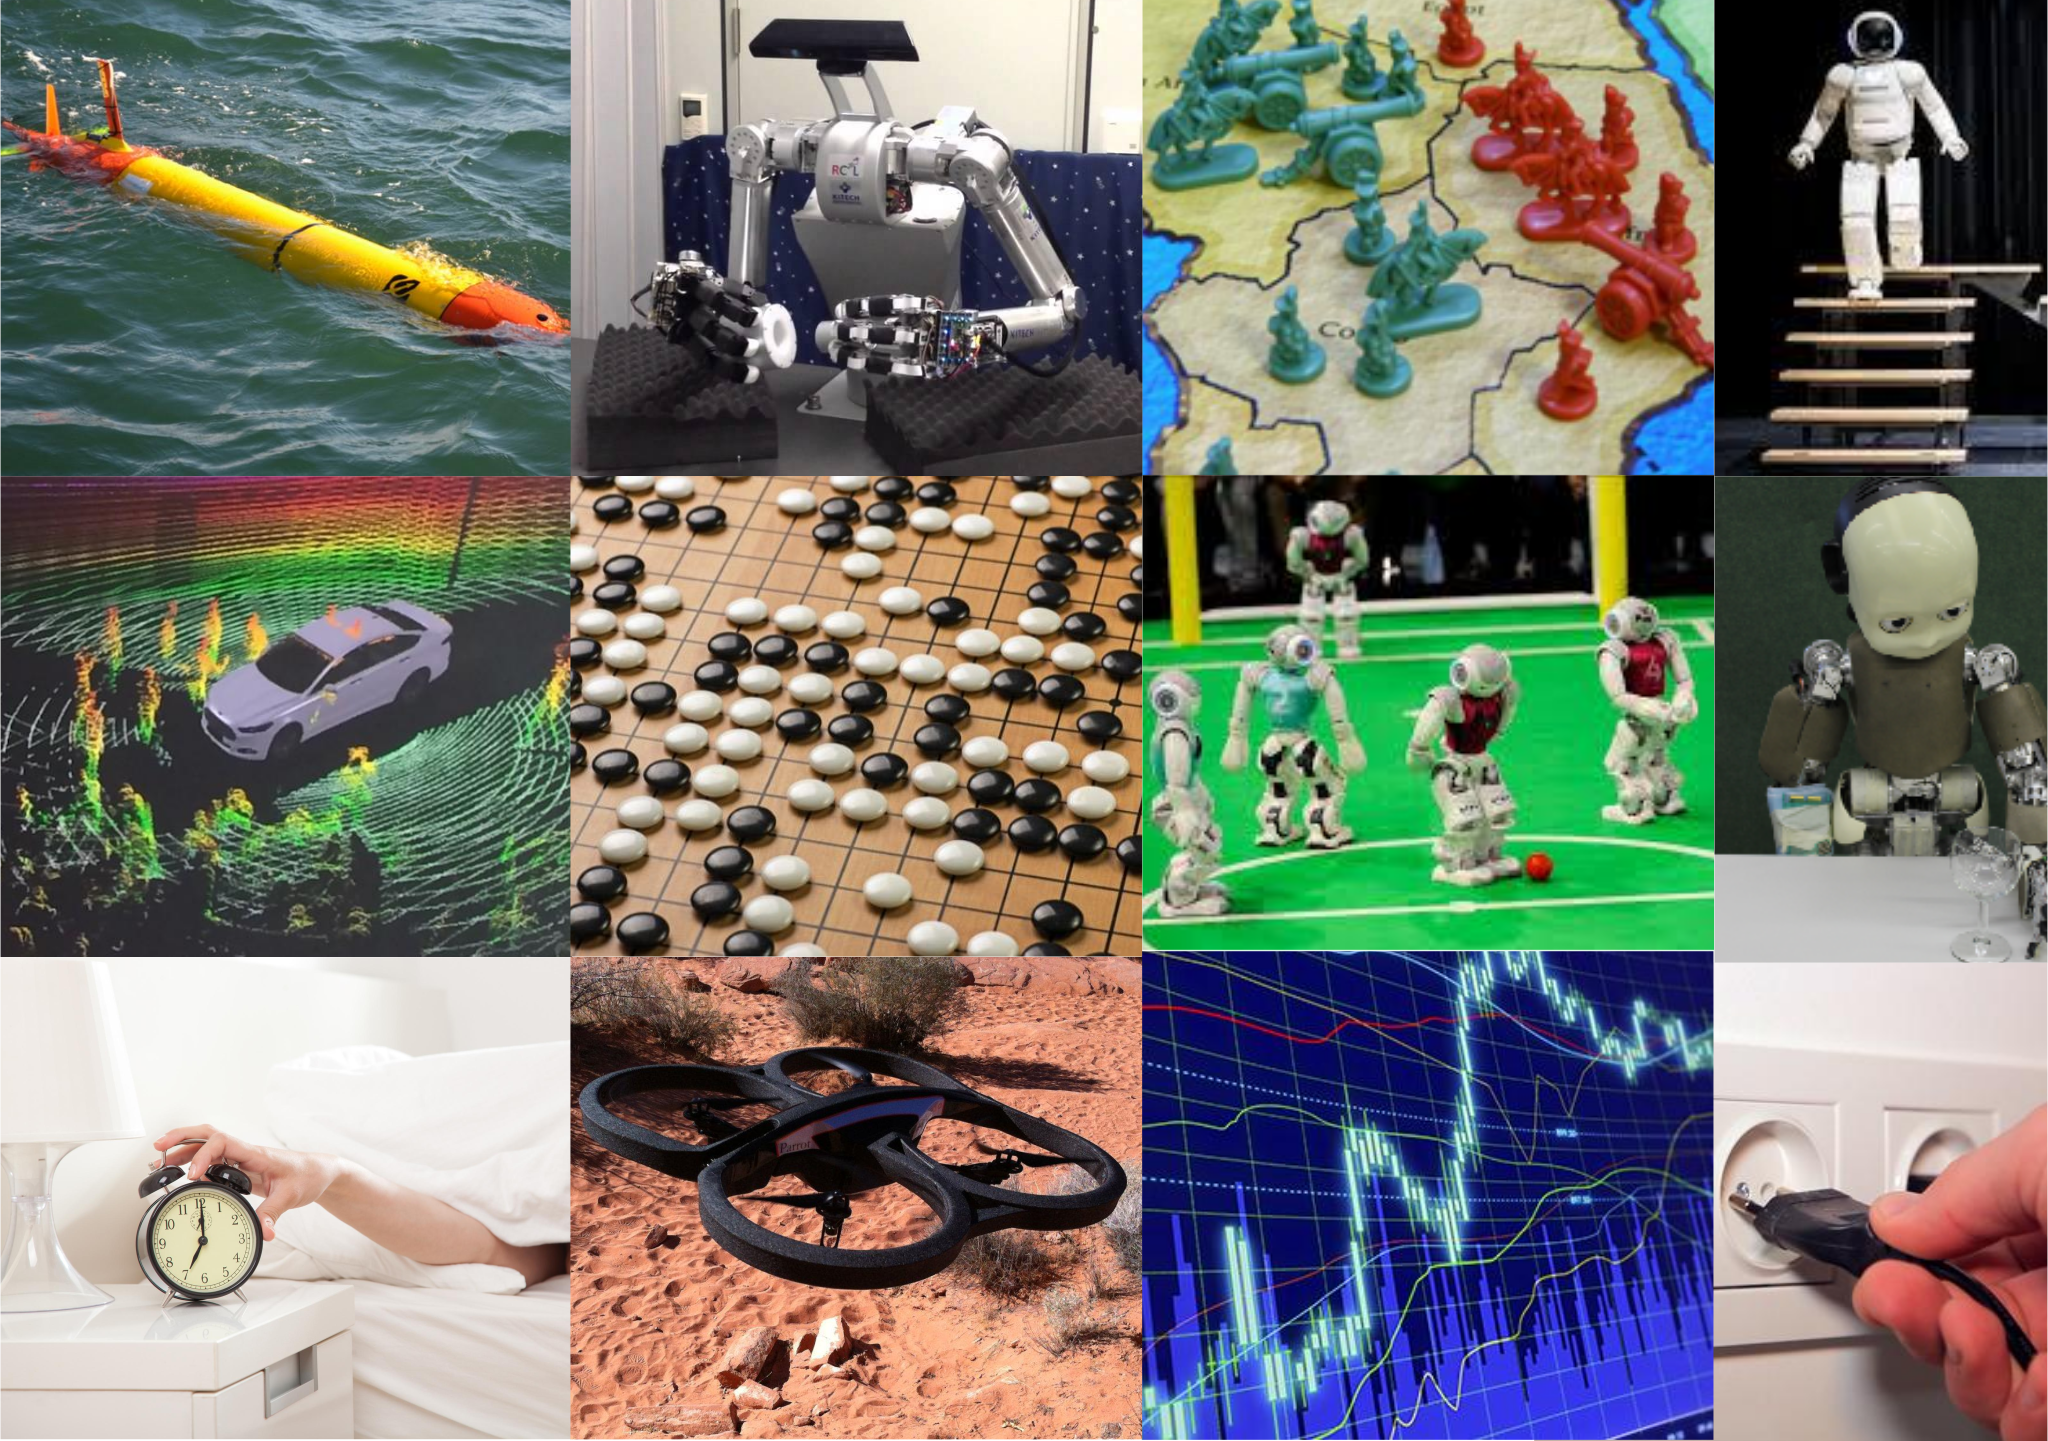
\includegraphics[width=0.9\textwidth]{examples.pdf}
 \caption{Examples of the decision making under uncertainty in both robotics and everyday life situations. Images taken from the public domain.}
\end{figure}

In summary there are still open problems in decision making when considering partial observability. The  mapping problem has been 
studied and solved within a certain set of constraining assumptions. For the mapping problem we develop a Bayesian filter which 
is non-parametric and has no explicit representation of a joint distribution.

Currently, both humans and animals are far better at navigation than robots, especially when uncertainty is present, \cite{stankiewicz2006lost}.
When addressing the decision making, we leverage human foresight and reasoning in a Learning from Demonstration (LfD) framework (\cite{Billard08chapter}), 
which is used to transfer skills from an expert teacher (usually a human) to a robot. Examples include the transfer of 
kinematic task constraints, stiffness and impedance constraints and motion primitives, to name only a few.

In this thesis we address both problems under extreme levels of uncertainty. 


%The advantage of taking a LfD approach and encoding the demonstrated behaviour in a asynchronous dynamical system (ADS) is that we have robustness to perturbation
% and a generalisation over the entire state space. 

\section{Contribution}
% - One page 1/2 

In this thesis we bring to light two main ideas. The first is the transfer of human behaviour to robots
in tasks where a lot of uncertainty in present, making them difficult to solve using traditional techniques.
The second is a non-parametric Bayesian state space filter which is efficient under sparse sensory information 
and high levels of uncertainty.

Throughout the work in this thesis we consider case studies in which vision is not available, leaving tactile and 
haptic information. This choice was made to induce a high level of uncertainty making it easier to study its effect 
on the decision making process. As a consequence the tasks we consider are by nature, haptic and tactile searches.
The following three sections detail the contribution of this thesis to research decision making under sever 
uncertainty constraints.

\subsection{Learning to reason with uncertainty as humans}

A Markov Decision Process (MDP) allows the formulation of a decision problem in terms of states, actions, a discount factor 
and a cost function. Given this formulation and a suitable optimisation method (dynamic programming, temporal difference, etc..) 
a set of optimal decision rules are returned, known as a policy. The benefit of this approach 
is that the policy is non-myopic and sequences of complicated actions can be synthesised to achieve a goal which 
an opportunistic policy would fail to achieve. A Partially Observable Markov Decision Process (POMDP) is 
a generalisation of an MDP to a hidden state space and only observations are available relating 
to the state space. Finding an exact optimal solution to a POMDP problem is notoriously difficult due to 
the computational complexities involved. Sample based approaches to solve a POMDP rely heavily on 
a good trade-off between exploration and exploitation actions. Good explorative actions increase the chance of discovering 
a set of optimal decisions/actions.

%An exact solution to a POMDP is only feasible in simple toy problems 
%(\cite{Thrun_Burgard_Fox_2005}) and existing approximate solutions are tailored for discretized 
%representation of states, actions and observations and an optimal solution heavily relies on 
%the exploration-exploitation trade-off.

In this thesis we propose a Learning from Demonstration approach to solving POMDP problems in
haptic and tactile search tasks. Our hypothesis is that if we know the mental state of the human 
expert in terms of his believed location and observe his actions we can learn a statistical policy 
which mimics his behaviour. Since the human's beliefs are not directly observable we infer them 
by assuming that the way we integrate evidence is similar to a Bayesian filter. There is   
evidence both in cognitive and neuroscience that this is the case (\cite{Bake_Saxe_Tene_2011}). From 
observing the expert human performing a task we learn a cognitive model of the human's decision process 
by learning a generative joint distribution over his beliefs and actions. The generative distribution 
is then used as a control policy. By this approach we are able to have a policy which can handle uncertainty
similarly to humans. 

\subsection{Non-parametric Bayesian state space filter}

Simultaneous Localisation and Mapping (SLAM) is concerned with the development of filters to accurately and efficiently infer 
the state parameters of an agent (position, orientation) and aspects of its environment, commonly referred to as the map. 
It is necessary for the agent to achieve situatedness which is a precondition to planning and reasoning. The 
predominant assumption in most applications of SLAM algorithms is that uncertainty is related to the noise in the sensor measurements. In 
our haptic search tasks there is no visual information and a very large amount of uncertainty. Most of the sensory
feedback is negative information, a term used to denote the non event of a sensory response.
In the absence of recurrent sightings or direct measurements of objects there are no correlations from the measurement errors 
which can be exploited. 

In this thesis we propose a new SLAM filter, which we name Measurement Likelihood Memory Filter (MLMF), in 
which no assumptions are made with respect to the shape of the uncertainty (it can be Gaussian, multi-modal, uniform, etc..) and 
motion noise. We adopt a histogram parametrisation (this is considered non-parametric because a change in a parameter has a local effect). 
The conceptual difference between the MLMF and standard SLAM filters, 
such as the Extended Kalman Filter (EKF), is that we avoid representing the joint distribution since it would entail a shattering space and time complexity. 
This is achieved by keeping track of the history of measurement likelihood functions. We demonstrate that our approach gives 
the same filtered marginals as a histogram filter. In such a way we achieve a Bayes filter which has both linear space and 
time complexity. This filter is well suited to tasks where the landmarks are not directly observable.

\subsection{Reinforcement learning in belief space}

We propose a Reinforcement Learning framework for the task of searching and connecting a power plug to a socket, with only haptic. 
We previously addressed this setup by learning a generative model of the beliefs and actions with data 
provided by human demonstrations following the LfD approach. However, it is usually the requirement that 
the teacher is an expert, with few notable exceptions (\cite{rai2013learning}). Since we were solely learning a 
statistical controller, both good and bad demonstrations will be mixed in together. By introducing a cost function 
representing the task we can explicitly have a quality metric of the provided demonstrations. In this way 
we can optimise the parameters of our generative model to maximise the cost function. In this LfD Reinforcement 
Learning setup with a very simple cost function we can have a significant improvement of our a policy.


\begin{figure}
  \centering
  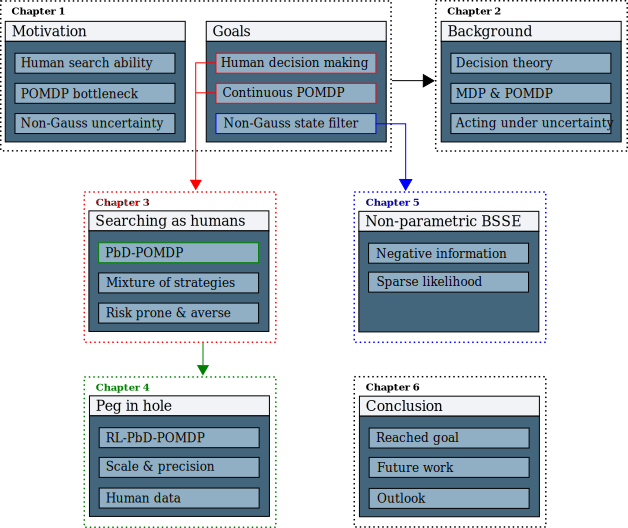
\includegraphics[width=\textwidth]{roadmap.pdf}
  \caption{Roadmap of the Thesis with key points. }
\end{figure}


\section{Thesis outline}

The thesis is structured accordingly to the three main contributions outlined in the previous section, 
and all will have their individual chapter. We outline below the structure of the thesis.

\begin{minipage}[c]{0.9\textwidth}
\paragraph{Chapter 2 - Background}\\
In this chapter we introduce and mathematically formalise the sequential decision making problem 
under uncertainty and we provide a detailed literature review of the related work in this domain.
We provide a brief introduction to \textit{Decision Theory} before focusing on the work 
in AI \& robotics relevant to POMDPs whilst highlighting their relevance and contribution to our work. 
\end{minipage}

\begin{minipage}[c]{0.9\textwidth}
\paragraph{Chapter 3 - Learning to reason with uncertainty as humans}\\
In this chapter we present an approach for transferring human skills in a blind haptic 
search task to a robot. The belief of the human is represented by a particle filter and 
all subsequent beliefs are inferred from the human's motions acquired via a motion tracking
system. A generative model of the joint belief and actions distribution is learned and used
to reproduce the behaviour on a WAM and KUKA robot in two search tasks. Experimental 
evaluations showed the approach to be superior to greedy opportunistic policies and traditional
path planning algorithms. The major parts of this chapter have been presented \cite{Chambrier2014}.
We also provide a review of work related to humans taking decisions under uncertainty 
in spatial navigation and haptic tasks with an emphasis on works which consider diminished or no 
visual information. 
\end{minipage}


\begin{minipage}[c]{0.9\textwidth}
\paragraph{Chapter 4 - Non-parametric Bayesian state space filter}\\
In this chapter we present an approach to perform a state space estimation of a map and agent 
given that there is no direct observation between the landmarks and the agent. We demonstrate that 
by not explicitly parametrizing the full joint distribution of the landmarks and agent but instead
keeping track of the applied measurement functions we can fully reconstruct the optimal Bayesian 
state estimation. The advantage of our approach is that the space complexity is linear as oppose 
to exponential. We validate our approach in 2D search navigation tasks. This work is currently under review.
We also give an overview of the literature of SLAM and emphasis the position of our filter within it.
\end{minipage}

\begin{minipage}[c]{0.9\textwidth}
\paragraph{Chapter 5 - Reinforcement learning in belief space}\\
In this chapter we present an approach similar to the one presented in Chapter 3, ``Learning to reason with uncertainty as humans'', with the difference that
we explicitly encode the task through the introduction of a binary objective function and we consider a peg-in-hole
task under high levels of uncertainty. The task requires both high and low levels or precision to be able to accomplish it,
which makes it particularly interesting. We learn a value function approximation of the belief space through locally weighted 
regression and approximate dynamical programming.
By combining a LfD approach in this Actor-critic Reinforcement Learning framework, we demonstrate an improvement upon 
a purely statistical controller with nearly no additional cost. 
We additionally provide a review of RL methods in the context of POMDPs.
\end{minipage}

\begin{minipage}[c]{0.9\textwidth}
\paragraph{Chapter 6 - Conclusion}\\
We conclude by providing a holistic summary of our work and achievements. We draw attention to the current 
open problems and directions for future work in field of uncertainty and reasoning in Artificial intelligence and robotics.
\end{minipage}







 	\fi
\ifdefined  	\gDisplayBackground		\chapter{Background}

% Introduce what is planning under uncertainty
Planning and reasoning under uncertainty is central to robotic and artificial intelligence research and has 
been an active area of research for decades. It is an umbrella term which touches a
wide spectrum of fields: \textit{economics}, \textit{psychology}, \textit{cognitive science}, \textit{neuroscience},
\textit{robotics} and \textit{artificial intelligence}. The work in this thesis relies on results  and assumptions 
made in cognitive and neuroscience with respect to our beliefs and how we act given them. We complement 
these results by introducing them in a new light to the field of robotics and demonstrate how the human reasoning and belief system 
can be used in situations where the state space is partially observable. The second main theme our work builds on is 
state space estimation. The third component acting given uncertainty in robotics. We make use of results from all 
three fields. We provide a background overview of acting under uncertainty and situate our work within the state of the 
art.

This chapter unfolds as follows: 



\section{Decisions under Uncertainty}
% What is the the reasoning under uncertainty planning problem
% What are all the assumptions which can be made regading the belief

In this section we introduce and frame the problem we seek to solve in generic 
terms. We are concerned with finding a sequence of actions which will lead to the successful 
outcome of a problem being considered; this is the most generic definition. 

There are two key attributes which can make this problem difficult: stochastic actions and latent states. Stochastic 
actions, when applied in the same state will not always result int the same outcome. This type of uncertainty 
can arise from many sources; the outcome of chaotic actions are impossible to predict with certainty, 
think of throwing a die or flipping a coin; In outdoor robotics the terrain might lead to slippage, causing 
the robot to skid or underwater currents might drastically offset the position of an UAV; In articulated 
robots the friction between joints can accumulate to a large error in the end-effector position (especially true 
for cable driven robots). 
The second source of uncertainty is when the underlying state is partially known, in the sense that we do not 
have all the necessary information to reliably determine the state beyond reasonable doubt. In robotics this 
uncertainty can arise from inadequate or noisy sensors. If the environmental conditions in which the robot 
is located is humid, misty or dark. It can make it difficult for the robot to ascertain its position and 
to plan how to achieve a given objective.

The uncertainty of the state and actions have to be quantified. The predominant approach 
is to  represent them by probabilities. For instance the application of a forward action (for a wheeled robot) 
will result in a new position further ahead and a position to the right (due to slippage) with some probability.
An observation through the robots sensors will result in probability distribution over the robots probable location.
Given this quantification of action and observation uncertainty in terms of a probability distribution over the state, 
the agent must now take actions towards accomplishing its goal. To take a decision the agent must assign a utility 
to the outcome of his actions. The utility is to indicate a preference over the outcomes and when combined with 
probabilities leads to decision theory. 

\subsection{Decision theory}

The central question of decision theory is; \textit{how do we take decisions when faced with uncertain outcomes ?} To answer
such a question we need to ground the attributes which are involved when we take a decision, namely our \textbf{beliefs} and 
\textbf{desires}. Beliefs reflect a degree of knowledge we have about the world in which the degree is ascertained by 
the amount of evidence we have in support of our beliefs. Epistemology studies in great detail the relationship between 
truth, beliefs and knowledge. We will not go into a philosophical discussion of their interplay, but make use of the following; 
if we have sufficient evidence in support of our beliefs and they represent the truth then we consider them to 
be a \textbf{rational belief}. As for desires they are linked to our disposition to take action to achieve them; for 
example if I want to switch of my alarm clock I have to look for it in the last area I believed it to be. 
These two attributes, beliefs and desires, are used to frame a decision problem. Early work in decision theory assumed 
that the problem was well grounded and focused on finding what are the \textbf{rational choices} to take given our beliefs 
to achieve our desires. 

\begin{figure}
 \centering
 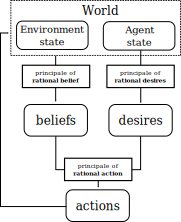
\includegraphics[width=0.5\textwidth]{/home/guillaume/Documents/Thesis/ch2-Background/Figures/cognitive_loop.pdf}
  \caption{ad}
\end{figure}

Early interest in such questions were typically centred around economics such as deciding what should be an appropriate 
investment or wager for a particular gamble. It was noted that the expected monitory outcome of a gamble as a mean of basing a 
decision, would often lead to a course of action which contradicts common sense; a famous example is the St. Petersburg paradox.
In this paradox a bookmaker proposes you the following gamble. An initial pot starts with a content of 2\pounds, the bookmaker proceeds 
to flip a fair coin until the first appearance of a tails which ends the game. Until the occurrence of the first tails 
the money in the pot doubles after every toss. Once the game ends you leave with the content of the pot. As an avid gambler 
and expected value maximiser how much would you be willing to pay to enter this gamble ? A value maximiser would computed 
the expected monetary outcome. The amount of money increases by $2^{n}\pounds$, where $n$ is the number of non-final tosses and 
and the probability of reaching $n$ is $1/2^{n}$. In this case the expected monitory outcome is an infinite number,

\begin{equation*}
\displaystyle \mathop{\mathbb{E}}_{p(n)}\{\pounds\} = \underbrace{\frac{1}{2} 2 \pounds}_{\textrm{first toss}} + \frac{1}{4} 4 \pounds + \dots = \sum\limits_{n=1}^{\infty} 
\frac{2^{n}}{2^{n}}\pounds = \infty \pounds 
\end{equation*}

So your expected gain or return for paying to enter such game is an infinite amount of money, so in principal if you were
seeking to maximise your expected return value you would be willing to pay an amount close to infinity. This does not 
seem a good decision rule; no person in the world would be willing to pay more than $1\pounds$ to enter such game.

Nicola Bernoulli proposed a solution to the problem (later published by his brother Daniel  (\cite{Bernoulli1954})) by introducing the notion 
of a \textbf{utility function}, and he claimed that people should base their decision on the expected utility instead 
of solely the monetary outcomes of a gamble.

\begin{quote}
  \onehalfspacing% <--- Local line spacing
  ``...the value of an item must not be based on its price, but rather on the utility it yields."\par\raggedleft--- \textup{Daniel Bernoulli}
\end{quote}

The introduction of a utility function takes into account that the net worth of a person will influence their decision since 
different people (in terms of their monetary worth) will weigh the gain differently. The utility function introduced by Bernoulli 
was the logarithm of the monetary outcome $x \in X$ weighted by their probability $p(x)$ which results in an expected utility, 

\begin{equation*}\label{eq:exp_utility}
  U(x) = \displaystyle \mathop{\mathbb{E}}_{p(x)} \{ u(x) \} = \sum_{x\in X} p(x) \underbrace{\log(x)}_{u(x)}
\end{equation*}

Different utility functions characterise different levels of risk. When the it is concave as it for Bernoulli's utility function
the person will be \textbf{risk-averse}, when linear \textbf{risk-neural} and convex \textbf{risk-seeking}. 
This was the first introduction of a utility function.

It is later in 1944 that von Neumann and Morgenstern (\cite{VonNeumann1944}) axiomised Bernoulli's utility function 
and proved that if a decision maker has a preference over a set of lotteries\footnote{the term lottery refers 
to a probability distribution in the original text.} which satisfy four axioms
(completeness, transitivity, continuity, independence) then there exists a utility function who's expectation 
preserves this preference. An agent whose decisions can be shown to maximise the vNM expected utility are said 
to be \textbf{rational} and otherwise \textbf{irrational}.  This is the theoretical basis of most economic theory,
it is a \textbf{normative} model of how people should behave given uncertainty. It is also the basis of most 
if not all decision making, cogitative architectures and control policies in AI and robotics 
(to the best of the authors knowledge).

An aspect to keep in mind regarding the vNM model is that it is normative; it states what should be a rational decision 
or behaviour. As a result it is not always consistent with human behaviour. There is great debate regarding 
the predictions made by vNM models with respect to ours. There have been many studies both demonstrating divergence 
between the models predictions and our observed behaviour but also supporting evidence that it does reflect 
the output of our decision making process. Reasons for divergence have been attributed to the way we 
weigh probabilities and how the decision problem is framed. But probably the most important aspect is that 
in most decisions we are faced with the quantification and rationality of our beliefs might not be adequate
and limitations of our working memory will come into play in the final decision.

Nevertheless vNM agents are predominantly used in AI and robotics as a means of implementing 
a decision making process or a control policy. In psychology and cogitative science vNM agents
are a used for comparing human behaviour against an optimal strategy (by optimal we mean it is rational in 
the vNM sense). 

%(see prescriptive models(\cite{Kahneman79prospecttheory}). 

% vNM is concerned with a one shot only decision, but what if we have to take a sequence of decisions ? What 
% happens then ?

%How is the uncertainty quantified ? Answer: probability theory
%How does the agent make a decision ? He must assigned a preference to the outcome of various actions
%Utility theory and combined with probability lead to decision theory.

% Speak about the historical context of plannig un
% Uncertainty and rational actions


% vNM theorem is limited to evaluation options that come with an 
% objective probability distribution over outcomes.
% a situation decision theoriests and economists often describe 
% as ''choice under risk``

% The utility function represents the agents desires.
% so the probability function represents her beliefs.
% The theories are referred to collectively as subjective expected utility (SEU).

% How is decision theory used in robotics ?


\subsection{Beliefs \& desires}

% POMDPs provide a rich framework for sequential decision-making under uncertainty in stochastic domains.
% Solving a POMDP is often intractable.

%\begin{enumerate}
% \item Decision theory
% \item Markov Decision Process
% \item Partially Observable Markov Decision Process
%\end{enumerate}

\begin{table}
\begin{center}
\renewcommand{\arraystretch}{1.5}
\begin{tabular}{|l|p{9cm}|} 
\hline
    \textbf{Notation} 			 	& \textbf{Definitions} \\ \hline\hline
    $x_t \in \mathbb{R}^3$ 		 	& Cartesian state space position of the agent.\\
    $y_t \in \mathbb{R}^{M}$		 	& Observation/measurement from the agents sensors.\\
    $a_t \in \mathbb{R}^3$		 	& Action, usually the Cartesian velocity of the end-effector of the agent.\\
    $X,Y,A$				 	& State, observation and action random variables where $x$, $y$ and $a$ are realisation.\\
    $p(x_t)$ 					& Short hand notation for a probability density function, $p_{X}(x_t)$.\\
    $x_{0:t}$					& $\{x_0,x_1,\cdots,x_{t-1},x_t\}$, history up to time $t$.\\
    $p(x_t|y_{0:t},a_{0:t})$	 		& Filtered probability distribution over the state space given the action and observation history.\\
    $b_t \in \mathbb{R}^{L}$			& Belief state, a function of the filtered distribution 
						 $b(p(x_t|y_{0:t},a_{0:t}))$ which will be written as $b_t$ for simplicity.\\
    $\policy(a_t|\cdot)$ 				& Probabilistic policy, $a_t \sim \pi_{\boldsymbol{\theta}}(a_t|\cdot)$ \\
    $r(x) \in \mathbb{R}$			& Reward function, returns the utility of being in state $x$. It can also be dependent on the action, $r(x,a)$.\\
    $\gamma \in [0,1)$				& Discount factor, the closer to one the more later utilities/rewards are considered. When set to zero, only immediate rewards are 
						  considered which would result in a myopic greedy agent.\\
    $p(x_{t+1}|x_t,a_t)$			& State transition function, returns the likelihood/probability of reaching state $x_{t+1}$ given that action $a_t$ is applied in state $x_t$.\\	
    $p(y_t|x_t)$				& Observation/measurement model, returns the likelihood/probability of observing $y_t$ given that the agent is in state $x_t$.\\
    $\tau(b_{t-1}(x),u_{t-1},y_t)$		& Updates a belief given a motion and observation, it makes use of both the motion and observation functions. The state space estimation function, $\tau$, can be any kind of state space filter such as an Extended Kalman Filter (EKF) or a Particle Filter (PF).
    \\ \hline
\end{tabular}
\end{center}
\caption{Definition of common variables used.}
\label{tab:notation}
\end{table}


\section{Sequential decision process}

When referring outright to decision theory with no extensions, we usually are talking about a one-shot
non-temporal decision. However many interesting decision problems are sequential.
In such a situation we must consider the effect current decisions will have on future decisions. Expected utility 
theory (part of decision theory) is extendible to a temporal decision problem. There are however a two subtle but important 
differences between the temporal and non-temporal decision problems. The first is the utility, in the one time step problem 
an outcome has one utility assigned to it, $u(x)$. Now a utility has to be assigned to a sequence of outcomes, $u(x_{0:T})$, 
where $T$ is the number of sequential decisions taken. The utility of a sequence is the sum of the individual outcomes 
themselves. However if the decision problem is non terminating this will lead to an unbounded utility. To bound the utility a 
discount factor $\gamma \in [0,1)$ is introduced and the new utility function becomes:

\begin{equation}
    u(x_{0:T}) 	   = \sum\limits_{t=0}^{T} \gamma^{t} u(x_t) \label{eq:joint_state_actions_util}
\end{equation}

The discount factor allows to control the importance later utilities have on the final utility. If the discount factor is set to
zero we recover the original one-shot utility function and if we were to take actions which maximised the expected utility 
we would not be considering at all the effect later decisions have on our overall utility. An agent reasoning in such a way is 
called myopic.
The second is the way in which probabilities are assigned to outcomes, this was $p(x)$ in the decision theory utility function formulation.
Now because of the sequential nature of the problem we consider a conditional state transfer probability distribution $p(x_{t+1}|x_t,a_t)$
which models the probability of going from state $x_t$ to $x_{t+1}$ given that action $a_t$ is taken. This particular representation of a
sequential decision problem is called a \textbf{Markov Decision Process (MDP)} and to be more exact a first order MDP.
The necessary models are the state transition and utility functions. The assumption of such a model is that all necessary information to 
take a decision is encoded in the current state and there is no need to consider the history of state transitions when taking a current decision.
In Figure \ref{fig:mdp} we illustrate two graphical representations of a MDP, which are known as \textbf{Dynamic Bayesian Networks (DBN)}.
A DBN represents the the temporal relationship and conditional dependence between random variables, decisions and utilities, which are 
represented by circles, squares and diamonds. For the MDP to the left the actions are not stochastic, whilst for the MDP on the right 
the actions taken are governed by a stochastic \textbf{policy}, $\policy(a_t|x_t)$. A policy represents the decision process of an agent,
given a state it will output an action. A stochastic policy means that given the same input they will produce
different outputs. A policy is considered optimal when it maximises the expected utility function, it is optimal in the vNM sense.

\begin{figure}[h]
  \centering
  \subfigure[off-policy]{\label{fig:mdp_off}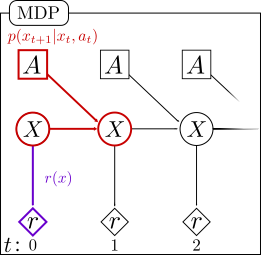
\includegraphics[width=0.45\textwidth]{/home/guillaume/Documents/Thesis/ch2-Background/Figures/mdp3.pdf}}
  \subfigure[on-policy]{\label{fig:mdp_on}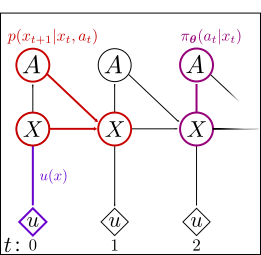
\includegraphics[width=0.45\textwidth]{/home/guillaume/Documents/Thesis/ch2-Background/Figures/mdp2.pdf}} 
  \caption{Dynamical Bayesian Network of a Markov Decision Process; it encodes the temporal relation between the random variables (circles),
  utilities (diamond) and decisions (squares). The arrows specify conditional distributions. In \textbf{(a)} the decision nodes are not considered 
  random variables whilst in \textbf{(b)} they are. From these two DBN  we can read off two conditional distributions, the state transition distribution (in red) and the action distribution (in purple). }
    \label{fig:mdp}
\end{figure}

Solving a MDP means finding a policy whose actions in any given state will always maximise the expected utility. Such 
a policy is usually denoted as $\pi^*$, the optimal policy. As in decision theory, the expected utility is the utility 
of  a sequence of states $u(x_{0:T})$ weighted by its probability . The graphical representation allows to read off directly the probability 
of a sequence of state transitions and actions $(x_{0:T},a_{0:T-1})$, Equation \ref{eq:joint_state_actions}.
\begin{align}\label{eq:joint_state_actions}
  p(x_{0:T},a_{0:T-1}) &= p(x_{0}) \prod_{t=0}^{T-1} p(x_{t+1}|x_t,a_t) \\
  u(x_{0:T}) 	       &= r(x_0) + \gamma r(x_1) + \dots + \gamma^{T-1} r(x_{T-1})  + \gamma^T r(x_T)
\end{align}
We are interested in finding the sequence of action, $a_{0:T}$, which will maximise the expected utility function:
\begin{equation}\label{eq:temporal_expected_utility}
 \argmax_{a_{0:T-1}} U(x_{0:T},a_{0:T-1}) = \max_{a_0} \sum\limits_{x_1}   \cdots  \max_{a_{T-1}} \sum\limits_{x_T} \Bigg( p(x_{0:T},a_{0:T-1}) u(x_{0:T}) \Bigg)
\end{equation}
Solving the above directly in its current form would have an exponential complexity. By making use of the first order 
markov assumption and that current rewards do not dependent future rewards, the sums in Equation \label{eq:max_util} can be re-arranged and 
and recursive patter will emerge which we can take advantage off. Lets start from the last time step and move out of the sum all elements 
which do not depend on $T$ and $T-1$, which results in Equation \ref{eq:expansion}
\begin{align}\label{eq:expansion}
 &\argmax_{a_{0:T-1}} U(x_{0:T},a_{0:T-1}) =\max_{a_0} \sum\limits_{x_1}   \cdots  \max_{a_{T-2}} \sum\limits_{x_{T-1}} p(x_{0:T-1},a_{0:T-2})  \nonumber\\
 &\left( u(x_{0:T-2}) + \gamma^{T-1} \left( r(x_{T-1}) +  \gamma \max_{a_{T-1}} \sum\limits_{x_{T}} p(x_{T}|x_{T-1},a_{T-1}) r(x_{T}) \right) \right)
\end{align}
From the rearrangement we notice that Equation \ref{eq:expansion} has the same functional form as Equation \ref{eq:temporal_expected_utility}, 
except that the recursive component can be summarised by Equation \ref{eq:bellman}, which is known as 
the \textbf{Bellman} optimal equation.
\begin{equation}\label{eq:bellman}
 V^*(x_t) := r(x_t) + \gamma \max_{a_t} \sum\limits_{x_{t+1}} p(x_{t+1}|x_t,a_t) V(x_{t+1})
\end{equation}
For the terminal state $V_T(x_T) = r(x_T)$. The bellman equation is a means of solving a sequential decision problem 
through use of dynamic programming. It says the the utility of the current state is based on the immediate reward and 
the discounted maximum utility of the next state. Making use of this recursion reduced the computation complexity is 
quadratic in the number of states, $\BigO(T\, |A|\, |X|^2)$. To find the optimal value and subsequent policy an approach 
would be to repeatedly apply the bellman equation to each state until the value function converges. What makes the problem 
hard to solve is maximisation over the actions. This induces two problems, the first is that the optimisation is nonlinear 
and the second is that if the action space is continuous the maximisation will be expensive to compute.
This brings use to the two main approaches to solving a the MDP process: \textbf{off-policy} and \textbf{on-policy}.
Off-policy methods solve directly for the optimal value function $V^*(x)$ and perform the maximisation over the actions, \textbf{Value-Iteration (VI)}
is such a method. On-policy approaches find the optimal value and policy through repeating \textbf{policy evaluation} and
\textbf{improvement} steps. In the policy evaluation the value or utility of a policy is found through solving the on-policy version of the Bellman 
equation:
\begin{equation}\label{eq:on_policy_bellman}
  V^{\pi}(x_t) := r(x_t) + \gamma \sum\limits_{a_t} \policy(a_t|x_t) \sum\limits_{x_{t+1}} p(x_{t+1}|x_t,a_t) V(x_{t+1})
\end{equation}
In the policy improvement step the policy is made more greedy by maximising the value function. Through the repetition of these two 
steps both the value function and policy converge to the optimal. On-policy methods are preferred in settings where the action 
space is highly continuous, such as in robotics. Using dynamic programming is however not the method of choice since it requires 
multiple passes through the entire state space and for this it is necessary to have the model of the state transition a priori. 
Instead \textbf{Reinforcement Learning (RL)} methods are used to find an optimal value and policy. RL is a sample based approach
in which an agent interacts with the environment gathering examples of state transitions and rewards (the utility) and uses them 
to gradually solve the bellman equation.

We introduced the formulation of a sequential decision process in the form of a MDP model and showed how an optimal policy 
and value function are obtained through maximising the expected utility. The re-arrangement of the sums via
variable elimination allows to take advantage of a recursive structure present in the markov chain. The recursive component 
turns out to be the Bellman optimal equation, which when solved (via dynamic programming or reinforcement learning) results 
in an optimal value and policy function. A MDP models the uncertainty inherent in the state transition but not the uncertainty 
of the state. The MDP assumes that the state space is always fully observable, which is a strong assumption. In robotics the 
on bored sensors return an estimate of the state with a certain amount of uncertainty associated with it. To take this additional
uncertainty into consideration the MDP has to accommodate it. This leads to a Partially Observable Markov Decision Process (POMDP).





% Define box and box title style
\tikzstyle{white_box}  = [draw=black, fill=white, very thick,  rectangle, rounded corners, inner sep=10pt, inner ysep=20pt]
\tikzstyle{fancytitle} = [fill=white,draw= black, text=white,rounded corners=1mm,text=black]


\subsection{POMDP}
%\begin{equation}
% y_t =  \begin{bmatrix}
%       r    \\
%       \phi \\
%     \end{bmatrix} \in \mathbb{R}^2
%\end{equation}

A POMDP is a popular approach for formulating a sequential decision process in which both motion and observation 
uncertainty is considered. In this partially observable setting the agent does not know with exactitude the state of the environment,
but is able to observe it through his \textbf{sensors}. We mathematically define a sensor as being a function of the 
state space, Equation \ref{eq:sensor}.

\begin{equation}\label{eq:sensor}
  y_t = h(x_t) + \epsilon_t
\end{equation}

The sensor function $h(\cdot)$ can be linear or non-linear and the additive noise term $\epsilon_t$ can 
be Gaussian (usually the case), non-Gaussian, state dependent or not. In this setting the
state $x$ is a latent hidden variable and we can only get information about it via the observations, $y$. 
The uncertainty of the latent state is quantified in a probability distribution over the state space, $p(x)$. 
This probability distribution represents all the hypothetical positions in the world in which the agent can be. 
In Figure \ref{fig:belief_update_example} \textbf{(a)} an agent is located in a environment a in a yard 
containing a wall. Initially the agent is confident regarding his position; his state uncertainty $p(x_0)$ is low, represented 
by the blue probability density. However during a circular displacement the agent skids and the state uncertainty is increased 
by the state transition function, $p(x_{t+1}|x_t,a_t)$. To reduce the uncertainty, the agent takes a measurement, $y$, with 
his sensors which provide range, $r$, and bearing, $\phi$, information of the wall, see Figure \ref{fig:belief_update_example} \textbf{(b)}.
The agent uses the model of his sensor, known a priori, to deduce all possible locations in the world, $x$, where the current 
measurement could have originated from. This model is known as the measurement 
likelihood function, Equation \ref{eq:likelihood}

\begin{equation}\label{eq:likelihood}
 p(y_t|x_t) = \mathcal{N}(y_t - h(x_t);0,\Sigma)
\end{equation}
The measurement likelihood function makes use of the measurement function $h(x)$ and it models the noise 
in the sensor. In this case the parameters of the noise model, $\epsilon_t$, is Gaussian with mean zero and covariance $\Sigma$.
Typically the parameters of the measurement likelihood function are learned a priori.

\begin{figure}
  \centering
  \subfigure[]{\label{fig:motion_update}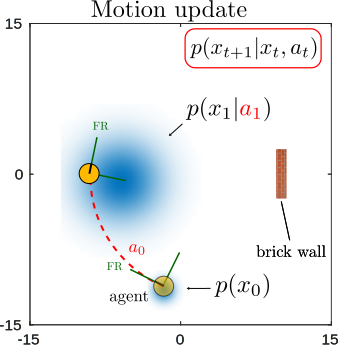
\includegraphics[width=0.45\textwidth]{/home/guillaume/Documents/Thesis/ch2-Background/Figures/motion_update.pdf}}
  \subfigure[]{\label{fig:measurement}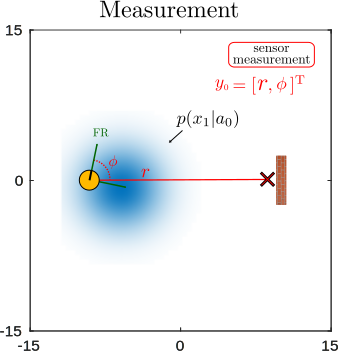
\includegraphics[width=0.45\textwidth]{/home/guillaume/Documents/Thesis/ch2-Background/Figures/measurement.pdf}} 
  \subfigure[]{\label{fig:likelihood}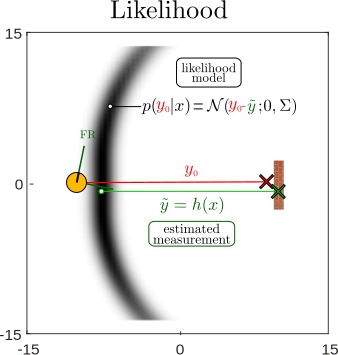
\includegraphics[width=0.45\textwidth]{/home/guillaume/Documents/Thesis/ch2-Background/Figures/likelihood.pdf}} 
  \subfigure[]{\label{fig:measurement_update}\includegraphics[width=0.45\textwidth]{/home/guillaume/Documents/Thesis/ch2-Background/Figures/measurement_update.pdf}} 
 \caption{\textbf{(a)} An agent is located to the south west of a brick wall, it is equipped with a 
  range sensor. The agent takes a forward action, but skids which results in a high increase of the uncertainty.\textbf{(b)} 
  The agent takes a measurement, $y_0$, of this distance to the wall; because his sensor is noisy his estimate is off. 
  \textbf{(c)} The agent uses with his measurement model to evaluate the plausibility of all locations in the world which would result in a similar
  measurement; illustrated by the likelihood function $p(y_0|x_0)$. \textbf{(d)} The likelihood is integrated into the probability 
  density function; $p(x_0|y_0) \propto p(y_0|x)p(x_0)$.}
  \label{fig:belief_update_example}
\end{figure}

In Figure \ref{fig:belief_update_example} \textbf{(c)} the likelihood is illustrated; the dark regions indicate areas of high 
likelihood, which are possible locations from which the sensor measurement could have originated from. The value of the measurement
likelihood function is then integrated into the state space probability density function.

These two steps: \textbf{motion}  and \textbf{measurement} updates are part of a state estimation process called a \textbf{Bayesian state space filter}, 
which we formalise below in Equation \ref{eq:motion_update}-\ref{eq:measurement_update}.
\begin{figure}
\centering
\begin{tikzpicture}
\node [white_box] (box){%
     \begin{minipage}{0.9\textwidth}
     The Bayesian filter turns a prior probability distribution over the state space, $p(x_t|y_{0:t-1},a_{0:t-1})$,
  to a posterior $p(x_t|y_{0:t},a_{0:t})$ by incorporating both motion and measurement. Applied recursively it 
  keep a probability distribution over the state space which considers all the past history of actions and observations.We define 
  the application of these two steps by the filter function $\tau$, which returns takes the current belief, applied action 
  and measurement to return the next belief, $b_{t+1}$.\\
  
  \textbf{Motion update}
	\begin{equation}\label{eq:motion_update}
	  p(x_t|y_{0:t-1},a_{0:t}) = \int p(x_t|x_{t-1},a_{t-1})\, p(x_t|y_{0:t-1},a_{0:t-1})\;da_{t-1}
	\end{equation}
      \textbf{Measurement update}
	\begin{align}\label{eq:measurement_update}
	  p(x_t|y_{0:t},a_{0:t})   &= \frac{1}{p(y_t|y_{0:t-1},a_{0:t})}p(y_t|x_t)\,p(x_t|y_{0:t-1},a_{0:t}) \\
	  p(y_t|y_{0:t-1},a_{0:t}) &= \int p(y_t|x_t)\,p(x_t|y_{0:t-1},a_{0:t}) dx_t
	\end{align}   
	\textbf{Filter function}\\
	\begin{equation}
	  b_{t+1} := \tau(b_t,a_t,y_t) 
	\end{equation}
    \end{minipage}
};
\node[fancytitle, right=10pt] at (box.north west) {Bayesian filter};
\end{tikzpicture}%
\caption{Bayesian state space filter.}
\end{figure}

The motion model, Equation \ref{eq:motion_update}, updates the position of the probability distribution according to 
the applied action, $a_t$, and adds uncertainty by increasing the spread of the distribution. The measurement information is 
the incorporated by Equation \ref{eq:measurement_update}. The measurement likelihood always decreases the uncertainty 
or leaves it constant. It never results in an increase of uncertainty. The Bayesian state space filter is such an important 
component to belief space decision making that we define it by the filter function, $\tau(b_t,a_t,y_t)$, which 
takes as input the current belief, applied action and sensed measurement and returns the resulting belief $b_{t+1}$.
The state space filter is an essential component to a POMDP as it will become apparent.

%Depending on the type of sensors: stereo cameras, infra red sensors, Kinect, 
%omnidirectional camera, etc.., there is uncertainty associated with it. It is thus important 
With the latent state and its relation to the observation variable and the Bayesian filter defined, we can introduce the POMDP model
in Figure \ref{fig:pomdp} (\textit{left}). It has the same markov chain structure 
present in MDP, introduced in the previous section, but the state space $X$ is latent and 
a new layer of observation variables $Y$ is present. 

\begin{figure}
 \centering
  \centering
  \subfigure[]{\label{fig:sub_pomdp}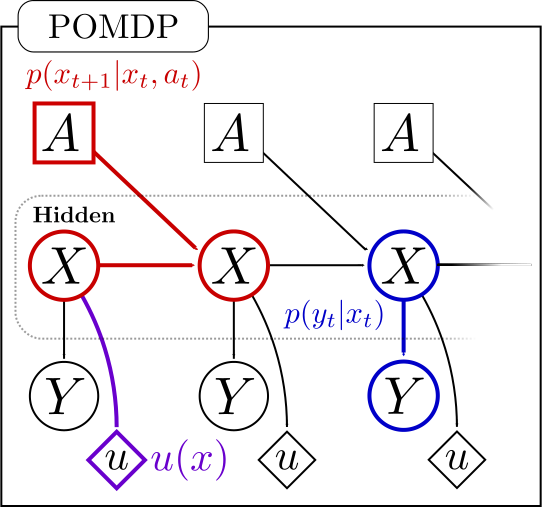
\includegraphics[width=0.45\textwidth]{/home/guillaume/Documents/Thesis/ch2-Background/Figures/pomdp2.pdf}}
  \subfigure[]{\label{fig:sub_bmdp}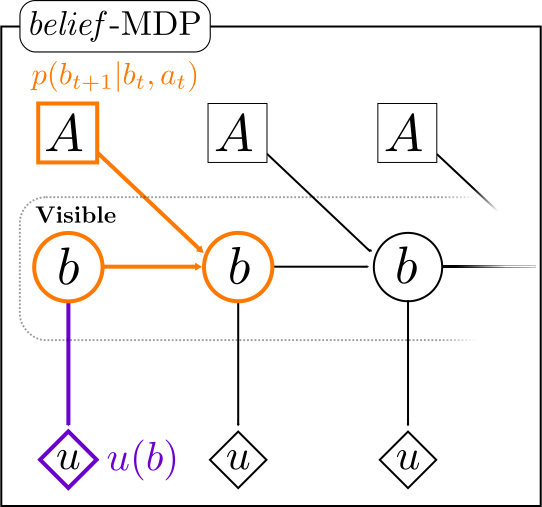
\includegraphics[width=0.45\textwidth]{/home/guillaume/Documents/Thesis/ch2-Background/Figures/pomdp3.pdf}} 
  \caption{\textbf{(a)} POMDP graphical model. The state space, $X$, is hidden, but is still partially observable through a 
  measurement, $Y$. \textbf{(b)} belief-MDP, the POMDP is cast into a belief Markov Decision Process. The state space is 
  a probability distribution, $b(x_t) = p(x_t)$, (known as a belief state) and is no longer considered a latent state. The original state 
  transition function $p(x_{t+1}|x_t,a_t)$ is replaced by a belief state transition, $p(b_{t+1}|b_t,a_t)$. The reward 
  is now a function of the belief.}
  \label{fig:pomdp}
\end{figure}

%We will see that because the state space is hidden it will cause complications to the maximisation of the expected utility.
%Since the states are not observable, the agent cannot choose its actions based on the state. The explicit 
%representation of the past events is typically memory expensive. Instead it is possible to summarize all relevant %
%information from previous actions and observations in a probability distribution over the state space, known as the
%belief state. 

Because the state space is partially observable the expected reward has to be computed for each possible history of states, actions and observations.
All approaches in the literature instead encapsulate all these possible histories into a belief state $b(x_t)$ (for short notation $b_t$)
which is a probability distribution (also referred to as an information state, \textit{I}-state) over the state 
space $x_t$ and use this new state description to cast the POMDP into a \textbf{belief-MDP} (states are probability distributions, 
beliefs). By casting the POMDP to a \textit{belief}-MDP the state space is considered observable and we recover the same structure 
as in the standard MDP problem.

Because we are working with in a belief-space the reward function has to be adapted to:
\begin{equation}
  r(b_t) = \int_{x_t} r(x_t)\, b(x_t)\;dx_t
\end{equation}
which is the expected reward $r(b_t) = \mathbb{E}_{b_t}\{r(x_t)\}$. The goal as before is to find a sequence of actions 
which will maximise the expected utility. Since our \textit{belief}-MDP has the same structural form as the MDP the solution 
to the problem is the same bellman equation equation derived previously. We just substitute the new belief transition function 
and we get the corresponding belief bellman Equation, \ref{eq:belief_bellman}.
\begin{equation}\label{eq:belief_bellman}
 V^*(b_t) = r(b_t) + \gamma \max_{a_t} \int_{b_{t+1}} p(b_{t+1}|b_t,a_t)\,V^*(b_{t+1})\;db_{t+1}
\end{equation}
Using this equation in this form is problematic, we are integrating over the space of beliefs and the 
transition function is a probability distribution over beliefs. The key to overcome this problem is to 
realise that if we know what the current measurement and applied action are there is only one valid possible belief.
Thus the integration over beliefs vanishes. This can be seen by substituting the belief transition function,
Equation \ref{eq:belief_state_transformation}, into the bellman equation Equation \ref{eq:belief_bellman}.
\begin{equation}\label{eq:belief_state_transformation}
 p(b_{t+1}|b_t,a_t) = \int_{y_t} p(b_{t+1}|b_t,a_t,y_t)\,p(y_t|y_{0:t-1},a_{0:t})\; dy_t
\end{equation}
After the substitution and re-arrangement of the sums we get an integral over all future value 
functions weighted by there probability, see Equation \ref{eq:max_component} which is the section of the bellman equation 
after the max. Since the observation is known (because the outer integral is over $y_t$),
the integral over the beliefs vanishes since there is only one possible future belief which is given by the 
Bayesian filter function $\tau(b_t,a_t,y_t)$.
\begin{equation}\label{eq:max_component}
 \gamma \max_{a_t} \int_{y_t} \underbrace{\left( \int_{b_{t+1}} p(b_{t+1}|b_t,a_t,y_t)\,V^*(b_{t+1})\; db_{t+1}\right)}_{1 \cdot V^*(\tau(b_t,a_t,y_t))}\, p(y_t|y_{0:t-1},a_{0:t}) \; dy_t
\end{equation}
In the final belief state bellman equation, the integral of the belief state is replaced by an integration over observations,
Equation \ref{eq:final_belief_bellman}.
\begin{align}\label{eq:final_belief_bellman}
  V^*(b_t) &= r(b_t) + \gamma \max_{a_t} \int_{y_t}  p(y_t|y_{0:t-1},a_{0:t}) \,V^*(f(b_t,a_t,y_t))\; dy_t \nonumber  \\ 
	   &= r(b_t) + \gamma \max_{a_t} \E_{y_t}\{V^*(f(b_t,a_t,y_t))\}
\end{align}
The belief bellman equation is intuitive, the value of the current belief is the immediate reward plus the value of the 
future belief states weighted by the probability of a measurement which would result in these future belief states. 
It turns out that computing a value function using the above bellman function is not computationally tractable. Solving 
a POMDP problem as for the MDP case consists of finding the optimal value function from which the optimal policy can 
be derived. Essentially the same dynamic programming and reinforcement learning techniques can be applied to solve 
this problem. An exact solution is however only  feasible when considering a finite state, action and observation space and
a finite planning horizon $T$. Most early techniques for solving POMDPs used value iteration. It has been shown (\cite{Sondik_1973}) 
that because the reward function uses a linear operator (the expectation) and that the bellman backup operation 
(applying the bellman equation to the current value function) preservers the linearity, the value function after each 
updates is piece wise linear and continuous (PWLC). The intractability comes from the successive applications 
of the bellman backup operation which result in an exponential time and space complexity with respect to the planning horizon.
A good text on the implementation of exact value iteration for POMDPs can be found \cite[Chap. 15]{Thrun_2005}
and here \cite{Kaelbling_1998}.

%From considering the decision belief tree of the POMDP, Figure \ref{fig:pomdp_bel_tree}, we can appreciate the complexity of the problem
%of finding an optimal policy. Given a discrete set of actions and observations to update the belief $b_1$ we have to consider a time 
%complexity of $\mathcal{O}(|U||Y|^T)$ where $T$ is the depth of the tree (the planning horizon). Given that we have a finite set of 
%belief the complexity solving the POMDP is $\mathcal{O}(|\mathcal{B}||U||Y|^T)$. 


%\begin{figure}[h]
% \centering
% 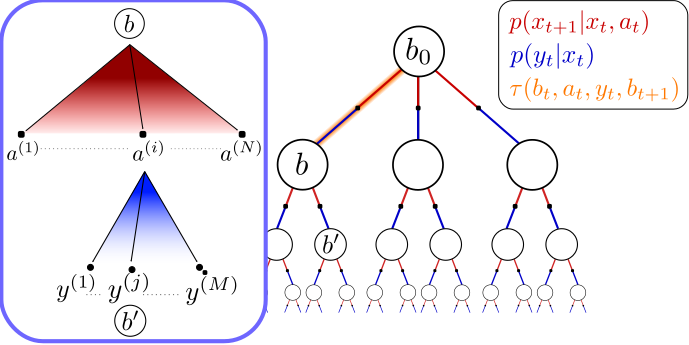
\includegraphics[width=\textwidth]{/home/guillaume/Documents/Thesis/ch2-Background/Figures/belief_tree.pdf}
%  \caption{ad}
%\end{figure}

Why is POMDP so good: combine information gathering and goal directed actions in one. Give taxonomy of planning under uncertainty here.
Finding a a solution to a POMDP is PSACE-complete (Papadimitriou & Tsitsikis, 1987), even when 
the dynamics are known. Thus approximate methods are needed for even the simplest problems.

\section{State of the art}

We review the latest methods of solving sequential decision problems under uncertainty. This is an extremely dense and spread out 
area of research, no doubt because of its importance and the fact that it cannot be ignored. If uncertainty is not considered 
adequately, the control policy risks being suboptimal or lead to drastic failure. 




\subsection{Point-based Value Iteration}

The POMDP formulation introduced previously is the main theoretical starting point of policies which
consider uncertainty. However solving an exact POMDP, problem through dynamic programming (value iteration) is 
computationally intractable and an exact solution only exists for discrete state, action and observation space \cite[Chap. 15]{Thrun_2005}.
This intractability, in which only problems with a few states could be solved, inhibited the application of the POMDP framework to robotics. 
The first breakthrough, Point-Base Value Iteration (PBVI) \cite{PBVI}, allowed to apply VI to a robotic navigation problems (626 states). The key insight 
which allowed VI to scale was to only consider a subset of the belief states which were reachable and relevant to the problem. This is achieved by smart sampling techniques
and only perform VI backups on beliefs states which are relevant. Before this point and before only value iteration on this subset instead of considering all beliefs.  If you 
have a $10 \times 10$ gird, this results in a total of a $100$ states and a belief state of a $100$ dimensions! The PBVI approach initiated a renewed effort in 
porting VI to POMDPs with larger and larger state spaces. From this point most research as focused on determining efficient strategies to sample belief points and
which to backup via VI. Heuristic Search Value Iteration (HSVI1) (\cite{HSV}) and HSVI2 (\cite{HSVI2}) uses forward search heuristic to find relevant beliefs by keeping a lower and upper 
bound on the current estimated value function. The belief tree gets expanded by choosing the action and observation whilst considering there potential future effect
on the value of the bounds, which thy try to minimise. It has equivalent results than classical PBVI with an exception to game of tag problem in which it fairs 
significantly better.  Later, Forward Search Value Iteration (FSVI) (\cite{FSVI}) takes an alternative approach than keepings an upper and lower bound on 
the value function, because doing so results in a drastically increases in the computation time necessary to find a solution. Instead they assume that the 
state space is fully observable, solve the the MDP problem and use this policy in the POMDP setting to generate a set of beliefs. It is orders of 
magnitude faster than HSVI and results in comparable polices. FSVI fairs badly however when information gathering actions are necessary. Since it is 
essentially using a myopic policy to generate it samples, these will be insufficient to find the global optimal policy when the solution requires 
information gathering actions. One of the very last sampling generation techniques which is considered to be the most efficient is SARSOP (\cite{SARSOP}),
it uses aspects present in both upper and lower bounds on the value function and the equivalent uncertainty free MDP solution to the problem. It tries
to sample belief points which will contain the optimal set of samples necessary to achieve an optimal policy.  Both SARSOP and HSVI2 are considered 
state of the art in PBVI value approximation techniques. (See \cite{POMDP_approach_2010}) for a review and comparison of both techniques on problems 
with thousands of states including simulation examples in grasping, tracking and UAV navigation. 

These methods are well suited to address problems which are easily expressed in a discrete state space. All considered problems are simulation based and 
no physical interaction problems are considers. Besides the belief set generation problem, interest has also been poised on porting the PBVI to a continuous state space.
A example of a continuous action space PBVI method is Perseus \cite{Spaan05icra}, in which the authors replace the maximisation over the action by instead sampling them from a 
parametric continuous representation. In \cite{PBVI_C_2006} the state space, transition and observation model are represented by Gaussian Mixtures and the authors consider a particle 
set or Gaussian mixture representation of the belief. The authors show that a continuous representation of the state space preserves the PWLC property of the value function. They extend 
there method to continuous action and observations through a sampling instead of discretising. Results are shown in 1D continuous corridor setting. In a 
more recent approach \cite{solving_continous_pomdps_2013} a discrete state presentation of a continuous state space is learned and is combined with sampling
techniques to solve the continuous integrals present in the bellman equation. The explicit learning of the state representation lead to an increased performance
when compared to the other continuous state PBVI methods and the others considered both continuous state and observation space. 

PBVI techniques have come fare since their first application to robotics navigation back in 2003 and have lead to a rapid increase of interest. 
Initially only a few hundred states could be considered and now problems with over ten thousand states are being solved in seconds. 
Most of the research has focused on how to gather efficiently a good set of sample beliefs. Later there have been efforts to expand PBVI 
to continuous state spaces such to be more suited to robotic applications. The main approach consists of using sampling techniques to overcome 
the maximisation over the actions (when considering continuous actions) or to choose a suitable parametric representation of the transition, observation 
and reward model such that the bellman equation can be solved in closed form. Most evaluation of have focused on simulated and simplified robotic 
navigation problems in 1D and 2D. We have not discussed online POMDP-solvers since there also based on VI and sampling techniques and thus share 
a lot of similarities with PBVI, we refer the reader to \cite{Ross08onlineplanning} for a detailed review.

%\cite{MCVI_CS_POMDPs}	% sampling techniques 

%Resent advances in PBVI methods: \cite{Veiga14aaai} 	   % Pedro Lima Point-Based method for Factor value 

% Point-based Value Iteration for Continuous POMDPs

\subsection{Parametric Value Iteration}

Point-based Value Iteration techniques tried to preserve the PWLC property of the value function. This directly 
leads to a discretization of the state space which if continuous by nature leads use prone to the curse of dimensionality.
An alternative approach is to represent the belief space by a parametric representation, for instance as a Gaussian function. 
The value function is then defined as a function of the parameters of the Gaussian. This approach in effect greatly 
diminishes the dimensionality problem but does away with the PWLC property of the value function. Instead to generalise 
the value of particular parameter a regressor function is needed and to learn it approximate dynamic programming techniques 
are used.

A very first successful example of this approach is \cite{MC-POMDP} were a POMDP problem in a continuous 
state, action and observation space was solved; with a working implementation on a physical mobile base.  
The belief was represented by a particle filter and the policy by a Q-value function, whose functional form was 
a non-parametric regressor (k-nearest neighbour) of the particle filter. The distance metric was the sample KL divergence
between two particle sets. The POMDP was solved through Reinforcement Learning (interaction with the environment) and 
approximated dynamic programming also known as experience replay, batch RL or Fitted Q-Iteration (FQI) \cite{Tree_batch_2005}. 
Although highly computationally demanding the method was successful. 

This lead to many similar approaches such as \cite{mc_update_ppomdps} where the belief state filter was an 
Extended Kalman Filter (EKF), the value function was also non-parametric and the POMDP was solved via FQI. 
When compared with Perseus in a discretized 2D localisation task both approaches reached equivalent 
policies but the authors method achieved it much faster than Perseus, a PBVI method. 

% 1) Belief space compression and value iteratrion
Another similar approach to parametrising the belief is to compress it to sufficient statistics and treat 
the decision problem as a fully observable augmented MDP (AMDP) in this new state representation. In \cite{Roy99coastalnavigation}
the authors compress the filtered belief to its mean and entropy and performed VI on this augmented state space
in a navigation task in which the goal was to reach a location with a minimum amount of uncertainty. This approach
brings a great simplification to solving the POMDP by at the cost of a lossy belief compression. In further developments
\cite{belief_compression_2005} compared both PCA and exponential-PCA (E-PCA, \cite{EPCA_2003}) as a means of belief compression techniques to find a low
dimensional belief space. This approach showed to be superior than the AMDP, it however requires transitioning back and forth 
between the low and high dimensional belief states. A step necessary for the the application of VI. The latest work in this 
area is \cite{bs_compression_2010} which investigates the use of nonnegative matrix factorisation in combination of k-means 
clustering as a means of compressing the belief which showed some improvement over the E-PCA approach but was only evaluated 
on discrete benchmark problems. Belief compression as mean of reducing the complexity of the belief state is interesting. The 
down side is that it requires discretising the belief to a fixed non-dynamic grid, collected many samples and learn an 
appropriate set of belief-basis eigenvectors. As such the larger the state space, the larger the dimensionality and thus more
samples are required to find a suitable set of basis.

% 2) A very large state space and do away with 
Recent developments lean more to the idea of very large state space representation and treat the problem as a MDP. In contrast to 
POMDPs there has been fare more research focused on MDPs and a lot of work has been done on the application of non-linear function 
approximators for representing the value function in combination with reinforcement learning optimisation techniques to solving them.
A successful example was the the usage of a multi-layer perceptron as a Q-value function approximator, Neural Fitted Q-Iteration (NFQ) \cite{neura_fqi_2005}.
This approach was successfully applied to the standard RL benchmarking problems (carte pole, acrobat, mountain care), but no partially observable
setting was considered. It is later in \cite{DRQ_AAAI_2015} that authors applied a Deep Recurrent Q-Network (DRQN) (extension to the work in \cite{mnih-dqn-2015})
to capture the history of states in a game of Pong where the state space was occluded half the time. By introducing a long term memory component 
the POMDP in effect is turned into a MDP and the authors apply an optimisation approach similar to FQI. 

Parameterization of the belief is a way of reducing the curse of dimensionality. By doing so the VI solution is no longer closed form and
function approximators are need to represent the value function. The value function is then optimised via approximate dynamic programming 
or reinforcement learning. These approaches are considerably more simple to implement than PBVI solvers which require heuristic pruning 
techniques and are difficult to port to continuous state spaces in general. There is a tendency to represent the POMDP has an augmented state MDP 
which then allows to apply well developed RL techniques. By using advanced non-linear function approximators the large state spaces can be 
handled in an efficient way and optimal policies can be found. However most of the applications seen so fare do no consider continuous actions
at all. Even for standard MDP the application of continuous action is problematic, which is due to need to maximise over the actions. We next
review a third approach of dealing with POMDPs which is more adapted to continuous actions. 

\subsection{Policy search}

The approaches seen so fare use a vale function to encode the problem which when solved a policy can be derived from it.
This requires learning a high dimensional value function over the belief space and the resulting policies are not necessarily 
smooth. This is because small changes in the value function can lead to drastic changes in the policy [cite]. There is no 
doubt that deriving a policy from a generic value function for highly continuous policy such in the case of controlling an
articulated robotic arm is no easy task. 
This has lead to development of an alternate approach in which a policy is learned directly without a value function. Instead
an initial policy is defined in terms of a parametrised function, $\policy$, and the utility is a function of the parameters, 
$u(\boldsymbol{\theta})$. The optimal policy is found by searching for the parameters $\boldsymbol{\theta}$ which will maximise 
the utility function. This is can be accomplished through various optimisation methods: gradient descent, expectation-maximisation, etc...

% Policy Iteration
%Early work include the application of policy iteration to a finite state controller \cite{p_search_pomdp_1998}. A finite state controller
%is iteratively evaluated (VI) and then subsequently improved until an optimal policy is found. Evaluation of the policy is much faster 
%than solving the optimal bellman equation, since the maximisation over the actions is absent. 

% Reinforce (gradient based methods)

% Actor-critic methods (combine both value function and policy)

% REINFORCE - PoWER - PI2 - 
One of the very first applied class of policy search algorithms were the REINFORCE (likelihood ratio) algorithms
first introduced by Williams \cite{reinforce_1992}. From a set of example episodes, also called roll-outs, the gradient
is estimated. The key aspect to this approach is that the derivative of the cost function is independent of the state
transition model and as a result the gradient is easier to estimate from samples. Application of this methodology 
to a partially observable setting lead to Gradient POMDP, GPOMDP \cite{gpomdp_2000} in which the authors developed 
a conjugate stochastic gradient ascent algorithm to optimise a policy with respect to the average reward. 

\cite{sis_pomdp_2002}


\cite{PoWER_2009}
\cite{NAC_2008}

%  Basically do gradient descent on parameters
\cite{Pegasus_2000}
\cite{heli_2004}

\cite{RL_robots_surv_2013}
\cite{p_search_surv_2011}

\cite{dmp_seq_2012} % PI2
\cite{dmp_iros_2011}


% Non pomdp method %Heurisitc: Information Gain
\cite{dense_entropy_icra_2014}
% Policy search
\cite{Uncer_reduction_heuristic_2015}
\cite{Sol_POMDP_Policy_space_1998}

\cite{sigma_hull_iros_2013}
\cite{int_motion_planning_2013}  % belief space planning


\subsection{Heuristics}

% Generic planning under uncertainty (not directly using a policy representation)
\cite{next_best_touch}
\cite{CostalNavigation1999}

\subsection{Planning}
$b = (\mu,\Sigma)$
\cite{Quadrator_2008},
\cite{BelRoadMap_2009}

\cite{non_gauss_bel_plan_2012}	% Non-Gaussian belief space planning
\cite{active_RSS_07} 	% Active Policy Learning for robot planning and exploration under uncertainty
\cite{plan_cont_bel_space_2015}
\cite{rob_online_bs_icra_2014}
\cite{bel_roadmap_2009}


\subsection{Optimal control}
$b = (\mu,\Sigma)$
 
\cite{plattRSS10} 	% Belief space planning
\cite{Erez10ascalable},
\cite{van_den_Berg_2012}, 
\cite{Platt-RSS-10}

 
% Grasping examples 
Grasping
\cite{u_aware_grasp_ICRA_2015}
\cite{learn_grasp_un_icra_2011}
\cite{seq_traj_replan_iros_2013}
\cite{Li_2015}

% Under water navigation examples

\cite{un_water_inspection_icra_2012}

% Continous

Optimal control methods represent the belief by a Gaussian function 

\cite{Bayesian_explor_exploit_2009}
% Sample based replanning
%\cite{Rand_belief_space_replanning} reference does not seem to exist
\cite{Macro_uncertainty_2011}

\section{Summary}




 	\fi
\ifdefined	\gDisplaySearch			\chapter{Learning to reason with uncertainty as humans}
%
%	Need to make this stick with the previous Chapter !
%
%	-> 
%
The conclusions drawn from the literature survey in Chapter 2 are that non-heuristic methods for planning and control 
rely heavily on the initial data provided to their respective optimisers. An ideal initial set of behaviour should be comprised
of explorative and exploitative actions so that a final optimal policy can quickly achieve the balance between minimising 
uncertainty and solving the task at hand. This is especially true for Reinforcement Learning (RL) methods which make use of 
explorative actions to be able to find an optimal policy. In many RL applications random exploration or Gaussian noise perturbation
is sufficient to find an optimal policy. This is the case when either an exhaustive search of the action space is possible 
(mountain cart, inverted pendulum, etc...) or in policy search methods where the policy is parametrised by a few parameters.
In continuous action-state space POMDPs, when a generic non-parametric policy is desired  this is not feasible, especially 
when the decision horizon is long. Continuous action-state space POMDPs applications have predominantly focused on cases in which 
the uncertainty can be quantized by a single Gaussian parametrisation. This representation can be constraining since it requires 
the observation likelihood to be Gaussian as well. This assumption is restrictive and ill-suited for haptic search tasks in 
which observations are discontinuous and occur as impulses. 

In this chapter, we demonstrate that human foresight and intuition can be leveraged as a means of solving the 
exploration/exploitation dilemma under partial observable conditions. Human beings are versatile in their ability to 
accomplish tasks which are considered to be complex by current robotic standards. This perceived ability which we have over 
current robotic systems, due to our prior domain knoweldge and experience, can be extracted, encapsulated and transferred 
to a robot apprentice.

To demonstrate the application of the transfer of behaviour from a human teacher to a robotic apprentice we apply the framework outlined in Chapter 2, 
Section \ref{sec:approach} (PbD-POMDP) to a blindfolded haptic search task. In our blindfolded search task, both a robot and a human 
must search for an object on a table whilst deprived of vision and hearing, illustrated in Figure \ref{fig:searching}. 
The robot and human both have prior knowledge of the environmental setup making this a specific search problem with no required mapping of the environment, also known as active localisation. 
In Figure \ref{fig:searching}, a human has his sense of vision and hearing impeded, making the perception of the environment partially observable and 
leaving only the sense of touch available for solving the task. The hearing sense is also impeded since it can 
facilitate localisation when no visual information is available and the robot has no equivalent giving an unfair 
advantage to the human. By impeding hearing we align the perception correspondence between the human and robot.

By representing the belief of the human's position in the environment by a Particle Filter (PF) and learning a mapping from this belief 
to hand actions (velocities) with a Gaussian Mixture Model (GMM), we can model the human's search process and reproduce it for any agent. 
We further categorize the type of behaviours demonstrated by humans as being either risk-prone or risk-averse and find that more than 70\% of 
the human searches were considered to be risk-averse. We contrast the performance of this human-inspired search model with respect to Greedy and Coastal Navigation search methods. 
Our evaluation metric is the distance taken to reach the goal and how each method minimises the uncertainty.
We further analyse the control policy of the Coastal Navigation and GMM search models and argue that taking  uncertainty
into account is more efficient with respect to distance travelled to reach the goal.

\begin{figure}[h]
  \centering
  \includegraphics[width=0.95\textwidth]{./ch3-Search/Figures/Figure1.pdf}
  \caption{\textbf{Blindfolded search task} \textit{Left:}  Search task, a human demonstrator searching for the green wooden block on the table given
  that both his hearing and vision senses have been impeded. He starts (hand) at the white spot near position (1). The the red and blue trajectories 
  are examples of possible searches.
  \textit{Middle:} Inferred belief the human might have with respect to his position. If the human always starts at (1) and his belief is known, all 
  following beliefs (2) can be inferred from Bayes rule. \textit{Right:} WAM Robot 7 DOF
  reproduces the search strategies demonstrated by humans to find the object.}
 \label{fig:searching}
\end{figure} 

There are \textbf{two assumptions} we make when applying Programming by Demonstration, PbD (also known as Imitation Learning), to the POMDP task described above. 
The first assumption is that the human teacher's \textit{spatial cognitive} abilities are good enough to accomplish 
the task in a consistent fashion. In other words demonstrations should not be random and a pattern exists. The second assumption is that human's beliefs inferred  
by the apprentice are close to the actual belief of the human. 

\section{Outline}

\begin{itemize}

\item  \hyperref[ch3:background]{\ref{ch3:background}   Background}\\
We review aspects of the literature in robotics and cognitive science which are related to spatial navigation which 
consider scenarios with limited perceptual information. We review related literature from \textit{Spatial Navigation}, 
\textit{Theory of Mind} and \textit{Programming by Demonstration}.

\item  \hyperref[ch3:experiment]{\ref{ch3:experiment}   Experiment}\\
The table search experiment protocols are described and we detail how to learn and transfer search strategies from human teachers to a robot 
apprentice. A total of 15 human teachers participated and each gave 10 demonstrations, giving a total of 150 searches.

\item  \hyperref[ch3:formulation]{\ref{ch3:formulation}  Formulation}\\
We detail the implementation of the human belief in terms of a Particle Filter (PF). This includes the measurement and motion 
models. We describe how we compress the belief particle filter in terms of the most likely state and differential entropy.

\item  \hyperref[chap3:policies]{\ref{chap3:policies} 	Policies}
\begin{itemize}
  \item \hyperref[chap3:GMM_policy]{\ref{chap3:GMM_policy} Modelling human search strategies}\\
  We detail the implementation and parametrisation of a Gaussian Mixture Model (GMM) policy encapsulating
the human search strategies and how it synthesises new searches.
  \item \hyperref[chap3:costal_policy]{\ref{chap3:costal_policy} Coastal Navigation}\\
  We detail the implementation of a Coastal Navigation policy, used as a comparison with the GMM policy.
\end{itemize}

\item  \hyperref[chap3:results]{\ref{chap3:results} 	Results}\\
We conduct three types of analysis: we quantify the behaviour present in humans and policies in terms of riskiness; we 
qualitatively evaluate the differences between the GMM policy learned from human demonstrations and the Coastal Navigation policy;
we evaluate the distance taken to find the goal for a set of four search policies, including the GMM.

\end{itemize}

\section{Background}\label{ch3:background}

%\subsection{Acting under partial observability}
%Learning controllers or policies to act within a context where the state space is partially observable is of high relevance to all real 
%robotic applications. Resulting from limited and inaccurate perceptual information, often only an 
%approximation of the environment is available at any given time. If this inherent uncertainty is not taken 
%into account during planning or control there is a non-negligible risk of missing goals, getting lost and 
%wasting valuable resources. 



%A major difficulty faced in spatial cognitive navigation and within the context of our PbD-POMDP framework is that 
%the biological and neurological processes which are responsible for the observed behaviour during the experimental studies 
%are unobservable. Even with the increasing usage of neuro-imaging techniques such as functional Magnetic Reasons Imaging (fMRI)
%and electroencephalogram (EEG), whose technical aspects impose limitations on the possible experimental studies, it is hard to 
%determine a cognitive mathematical model of the underlying processes present in spatial navigation. 

\subsection{Spatial navigation}
%
%	Take away points: 1) Humans and animals are currently better than robots in doing this.
%		          2) Limitations of the quality of our policy depend on our working memory.
%

Spatial navigation, \cite{Wang_2007}, \cite{what_det_our_nav_ability_2010}, focuses on the role that sensory perception 
(vision, vestibular, proprioception ...), motor control and mental cognition have on the navigational ability of  
humans, animals and insects. A central aspect of spatial navigation is the way in which we mentally represent the geographical world, known 
as a \textit{cognitive map} (mental representation of environment first proposed by Tolman, 1948) and how we update our pose estimation 
in this map. The aspects of both  construction and correction of a cognitive map have been studied in great depth, \cite{spatial_updating_2008}.
There is reported evidence that we use both vestibular and proprioception in inferring self-motion in order to update our position through dead reckoning (also known as path integration). 
Given the estimated position we then use external cues such as geometric (the shape of a room) and features (the colour of the walls), 
to correct our position. The actual representation of our position and environment in our cognitive map has been proposed,
\cite{spatial_memory_how_ego_allo_combine_2006}, to be either encoded in our own frame of reference (egocentric) or in a frame of reference which 
is independent to us (allocentric) and acts like a standard paper map or both. This cognitive map enables us to reason about the relations between our own position and that of other items and landmarks present. 
This representation also facilitates our ability to localise ourselves and plan novel routes when needed.

In \cite{updating_egocentric_human_navigation_2000}, the authors studied the effect that disorientation has on blindfolded subjects' ability 
to recover their heading, which is necessary for re-localisation. Through eight different experiments they concluded that humans 
have an egocentric cognitive map.


Studies have also looked at the difference between congenitally blind, late blind and sighted people in their ability to encode ego-allocentric cognitive maps.
In \cite{Pasqualotto2013175}, the authors dispose a set of seven objects (brush, slipper, pan, dish, book, spoon, bottle) in the form of 
an array in a 12.5m $\times$ 9m room. The objects are positioned on top of stools. During a training phase, ten congenitally blind, ten late blind and ten blindfolded sighted people were taken through 
the setup and touched all objects present. This guided exploration (the experimenter leading the subject through the object array) was repeated until 
the participants could correctly recall all the objects' locations twice consecutively without help. In a testing room (no objects present) 
the participants were asked ``Judgement of Relative Direction''  questions and the accuracy and response time were recorded. From the results the authors 
concluded that blindfolded and late blinded participants used a allocentric representation of the object array, whilst the congenital blind 
subjects use an egocentric model. The cause of this difference is attributed to the role played by vision in the development of the 
multisensory brain area, in which vision is necessary for the development of an allocentric model. 

Many similar experiments have been conducted and a summary can be found in the following review \cite{spatial_memory_how_ego_allo_combine_2006},
where the authors explicitly state that a consensus has formed; both egocentric and allocentric representations of the environment are 
working in parallel. Current questions ponder whether allocentric models are part of the semantic memory as opposed to the procedural 
memory used by the egocentric model.

\subsubsection{Spatial cognition and memory}

The quality of the human teacher in  search tasks, which are partially observable in the terms of absence of vision,
will strongly depend on the teacher's ability to maintain an accurate cognitive map of his environment. This implies
that the size of the environment and search task will have an effect on the teacher's ability to provide near optimal 
demonstrations. 
Early and influential research into human's short term memory was presented in 1956 by George Miller in a seminal work, \cite{cogprints730} 
(22'780 citations), in which he described the ``so called'' magical number of our short term memory as being $7\pm2$ items, 
known as \textit{Miller's Law}. This research was conducted on a one dimensional task in which no spatial navigation was required.
Since then there have been many studies investigating the limits of short term memory.

In \cite{human_stsm_2015} a set of subjects had to find either 1, 3, 5 or 7 goal pads, among a grid array of 23 pads in a 4m $\times$ 4m room, 
within a 1 minute interval. They measured the subjects' error in terms of the number of locations visited before finding the goals. 
They found that on average the subjects had to visit ``$1.6 \times \#num\_goals$'' pads before achieving the task. The authors concluded 
that in this spatial navigation task there was no magical number which represents the limit of short term memory.
In another spatial navigation experiment, \cite{Iachini2014}, the effect that the scale of the environment 
has on the ego-allocentric representation is studied in blindfolded, late and early blind subjects. The main findings were
that cognitively blind people have more difficulty in developing an allocentric representation of the world. 
%In terms of difference in the scale of the problem (two conditions where compared, a task which required no locomotion and one that did), 
%only a small difference existed for the blindfolded subjects.

In \cite{stankiewicz2006lost}, a search task in a virtual maze is conducted by a set of human subjects.  The aim 
is to investigate the limitations that perception, memory and uncertainty have on human decisions in comparison 
with an ideal agent (POMDP solution). The authors' main findings were that as the size of the maze increases the
performance of the human subject decreases with respect to the ideal agent, as human subjects are limited by the 
uncertainty in their location and have difficulty in maintaining multiple hypotheses.

\subsubsection{Summary: spatial cognition}


The studies detailed above reported that if the environment is not overly large and complex our cognitive model is sufficient 
to produce policies which are on par with an optimal POMDP agent. 

Our study seeks to transfer exploratory behaviour from human teachers to a robot apprentice in a partially observable setting. 
In our search scenario the environment is less than 3 meters in length and 2 meters in depth with a single goal object to be found. 
Given this setup and the evidence from previous studies, humans should be able to achieve this task with a high level of proficiency. 

This is beneficiary since currently both humans and animals are better at spatial navigation than robots \cite{stankiewicz2006lost} 
especially when uncertainty is present. The quality of the demonstrations will strongly depend on the teacher's short term memory 
in retaining a sufficiently accurate cognitive map of the environment. 


\subsection{Human beliefs}

% Belief  
%In the Section \ref{sec:deci_un} on Decisions in Chapter 2, we introduced the concept of rationality for 
%both beliefs and desires. 

A crucial aspect for the success of PbD-POMDP learning is that the apprentice be able to infer 
the human's belief of his location whilst he is searching. In others words the apprentice
(human or robotic) has to infer the cognitive map of the teacher. 

%This is possible by observing the actions of teacher and guessing his perception 

The study of inference of another's mental state is part of Theory of Mind (ToM) \cite{Towards_a_ToM_2010}, which is concerned 
with our ability to infer beliefs, desires, intentions, perception,
goals and current knowledge. In this study, the apprentice will have to infer the teacher's beliefs which we assume are 
\textbf{rational}. A rational belief is a belief for which observations bring supportive evidence and 
gradually increase the certainty of the belief. In a recursive formulation this known as Bayesian Theory of Mind (BToM),
where the Bayesian component highlights the hypothesis that humans integrate information and update their beliefs in a similar 
fashion to Bayes rule.

Due to the complexity in the number of sensory sub-components, such as gaze following, and their interplay, required as a precursor to the development
of a ToM, much effort has been focused their  development.
Early work in implementing a ToM in a humanoid robot was introduced in \cite{ToM_humanoid} and is based on ToM models of \cite{Leslie_TOMM} 
and \cite{Baron-Cohen}. The author focused on building basic skills such as face finding and distinguishing animate and inanimate 
stimuli but left open the problem of the final interaction between all the components.

In \cite{MRF_ToM}, the authors model ToM as a Markov Random Field which defines a joint probability distribution over a set of
hidden actions and observation variables. The functions of these variables are hand-crafted for each experiment. 
The authors demonstrate that through a suitable parameterisation of the MRF they achieve results comparable to the predictions of ToM.
Recently in \cite{ToM_HRI_2106}, ToM and planning architecture have been integrated in a joint action collaborative human robot task, 
in which position, goal and action state of the human partner is maintained by his robotic assistant.

% ????
Work on modelling human beliefs and intentions has been undertaken in cognitive science, \cite{Bake_Saxe_Tene_2011}, 
\cite{Richardson1_Baker1_Tenenbaum1_Saxe1_2012}. In \cite{Bake_Tene_Saxe_2006}, the authors present a Bayesian framework 
for modelling the way humans reason and predict actions of an intentional agent. The comparison between 
a generic Bayesian model and the humans' predictions yielded similar inference capabilities.
This when asked to guess the intentions of a goal oriented agent in a 2D world, which both the Bayesian model and the 
humans were observing. This provided evidence supporting the hypothesis that humans integrate information using Bayes rule. 
Further, in \cite{Bake_Saxe_Tene_2011}, a similar experiment was performed in which the inference capabilities of humans,
with regard to both belief and desire of an agent, were comparable to that of their Bayesian model. Again they found
the human's inference was comparable to that of the Bayesian model.

In our PbD-POMDP framework we make a similar hypothesis that humans integrate information in a Bayesian way, however in a 
continuous domain. We infer the belief that humans have of their location in the world during search tasks.

\subsection{Programming by demonstration \& uncertainty}

%% Programming by Demonstration  Imitation Learning
Programming by demonstration (PbD) is advantageous in the POMDP and MDP contexts since it removes the need to perform the time 
consuming exploration of the state-action tree to discover an optimal policy and does not rely on any exploration 
heuristics to gather a sufficient set of belief points (as in point based value iteration methods discussed in Chapter 2).

We expect humans to perform an informed search. In contrast to stochastic sampling methods, 
humans utilise past experience to evaluate the costs of their actions in the future and to guide their search. This foresight and experience are implicitly encoded 
in the parameters of the model we learn from the demonstrated searches.

PbD has a long history in the autonomous navigation community. In \cite{Kasper2001153}, behaviour primitives of 
the PHOENIX robot control architecture are incrementally 
learned from demonstrations. Two types of behaviour namely \textit{reactive} and \textit{history-dependent} are 
learned and are encoded by radial basis functions. The
uncertainty is implicitly handled by directly learning the mapping between stimulus and response. In \cite{Hamner_2006_5810} the parameters of a
controller which performs obstacle avoidance are learned from human demonstrations. The uncertainty is inherently handled 
by learning the relation between sensor input and control output. In \cite{LfD_Autonomous_Navigation_in_Complex_Unstructured_Terrain} the objective function of a path planner is learned from human demonstrations. 
The objective function is a weighted sum of features corresponding to raw sensor measurements. This is another example where the partial information of the state is 
taken into account at the perception-action level, with the difference that instead of a policy being learned the objective function from which it is generated is learned. 

% Uncertainty is in the dynamics
Uncertainty is not restricted to state estimations but can also present in dynamical interaction with the environment in which 
unforeseen and perceptual uncertainties can arise such as in manipulation tasks. When solely tracking a Cartesian trajectory 
position uncertainties (poor visual estimation of the target) can lead to the failure of the task or a dangerous accumulation 
of contact forces. In \cite{online_pre_sensor_2011} the authors learn, via imitation learning, an initial 
Dynamic Movement Primitive (DMP) Cartesian policy and separately a target a force profile. By using sensor feedback they 
modify the target trajectory such to replicate the force profile thus achieving robustness to pose uncertainty. Another possibility
is to vary the stiffness parameters of an impedance controller \cite{Klas_icra_2012} based on the position uncertainty, 
if the position uncertainty is high then the robot will be more compliant. In \cite{MedinaSH13} the authors introduce a 
risk-sensitive control framework which depending on the uncertainty will make a trade-off between the position and force errors parameter gains
of an impedance controller. The task (Cartesian position and velocity) which is tracked by the controller is learned from demonstrations and encoded in 
a model.

%In \cite{Nicolescu01learningand}, the authors learn how to combine low level pre-acquired action 
%primitives to achieve more complex tasks from human demonstrations, but 
%they do not consider the effect of uncertainty.



Much work has been undertaken in learning reactive-behaviour, history dependent behaviour and combining multiple behaviour primitives to achieve
complex behaviour. However very few have studied the effect of uncertainty in the decision process and 
do not consider it during the learning or assume that it is implicitly handled.
A noticeable exception is \cite{GeorgiosLidoris}, in which a human expert guides the exploration of a robot in an indoor environment. 
The high level actions (\textit{Explore}, \textit{Loop Closure}, \textit{Reach goal}) taken by the human are recorded along with three different features related to the uncertainty in the map. 
Using SVM classification a model is learned which indicates which type of action to take given a particular set of 
features. The difference with our approach is that we perform 
the learning in continuous action space at trajectory level and multiple actions are possible given the same state, which cannot be handled by a classifier.

%%%%%%%%%%%%%%%%%%%%%%%%%%%%%%%%%%%%%%%%%%%%%%%%%%%%%%%%%%%%%%%%%%%%%%%%%%%%%%%%%%%%%%%%%%%%%%%%%%%%%%%%%%%%%%%%%%%%%%%%%%%%%%%%%%%%%%%%%
%																	   %
%					Research Design and Methodology									   %
%																	   %
%%%%%%%%%%%%%%%%%%%%%%%%%%%%%%%%%%%%%%%%%%%%%%%%%%%%%%%%%%%%%%%%%%%%%%%%%%%%%%%%%%%%%%%%%%%%%%%%%%%%%%%%%%%%%%%%%%%%%%%%%%%%%%%%%%%%%%%%%

\section{Experiment: table search}\label{ch3:experiment}

In our search task setup, Figure \ref{fig:tab_search_task} and  Figure \ref{fig:experiment} (\textit{top left}), 
a group of 15 human volunteers were asked to search for a wooden green block located at a fixed position on a bare table. 
Each participant repeated the experiment 10 times from each of 4 mean starting points with an associated small variance. 
The starting positions were given with respect to the location of the human's hand (all participants where right handed). The humans were always facing the table with their right 
arm stretched out in front of them. The  position of their hand was then either in front, to the left, to the right, or in contact with the table itself. 

\begin{figure}
 \centering
   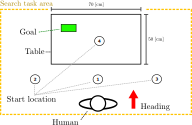
\includegraphics[width=0.8\textwidth]{./ch3-Search/Figures/experimentsetup}
  \caption{Table search task. Blindfolded human subjects after a disorientation step are placed in one of the 
  four starting locations. The heading of the subject is always kept the same. The human's objective is to locate
  the green block on the table. Throughout all experiments the green wooden block is kept in the same location.}
  \label{fig:tab_search_task}
\end{figure}
\begin{figure}
\centering
  \includegraphics[width=\textwidth]{./ch3-Search/Figures/Figure2}
  \caption{\textit{Top left}: A participant is trying to locate the green wooden block on the table
given that both vision and hearing senses have been inhibited. The location of his hand is being tracked by the
OptiTrack\textsuperscript{\textregistered} system. \textit{Top right:} Initial distribution of the uncertainty or belief we assume
the human has with respect to his position. \textit{Bottom left:} Set of recorded searches, the trajectories are with respect to the hand.
\textit{Bottom right:} Trajectories starting from same area but have different search patterns, the red trajectories all navigate to the goal
via the top right corner as opposed to the blue which go by the bottom left and right corner. Among these two groups there are trajectories which
seem to minimize the distance taken to reach the goal as opposed to some which seek to stay close to the edge and corners.}
\label{fig:experiment}
\end{figure}


As covered in the background section, previous work has taken a probabilistic Bayesian approach to model the beliefs and intent 
of humans. A key finding was that humans update their beliefs using Bayes rule (shown so far in the discrete case). 
We make a similar assumption and represent the human's location belief (where he thinks he is) by a particle filter which
is a point mass representation of a probability density function. There is no way of
knowing the human's belief with certainty. We make the critical assumption that the belief is observable in the first time step of the search and all following beliefs 
are assumed correct through applying Bayes integration.
The belief is always initialized to be uniformly distributed on top of the table, 
see Figure \ref{fig:experiment} (\textit{top right}), and the starting position of the human's hand is always in this area.

Before each trial the participant was told that he/she would always be facing the same direction with respect to the table (so always facing the goal, 
like in the case of a door) but his/her translational starting position would vary. 
For instance, the table might not be always directly in front of the person and his/her distance to the edge or 
corner could be varied. In Figure \ref{fig:experiment}
\textit{bottom left}, we illustrate four representative recorded searches whilst in the \textit{bottom right}, we illustrate a set of trajectories 
which all started from the same region. One interesting aspect is the diversity present,
demonstrating clearly that humans behave differently given the same situation.  

It is non-trivial to have a robot learn the behaviour exhibited by humans performing this task. As we cannot encapsulate the true complexity of 
human thinking, we model the human's state through two variables, namely, the human's uncertainty about his current location and the human's  
belief of his position. The various strategies adopted by humans are modelled by building a mapping from the state variables to actions, which are the motion of 
the human arm. Aside from the problem of correctly approximating the belief and its evolution over time, the model needs to take into consideration
that people behave very differently given the same situation. As a result it is not just a single strategy that will be transferred but rather a mixture 
of strategies. 


\section{Formulation} \label{ch3:formulation}

In the standard PbD formulation of this problem, a parametrised function is learned,
mapping from state $x_t$, which denotes the current position of the demonstrator's hand, to  
the hand's displacement $\dot{x}_t$. In our case since the environment is partially observable 
we have a belief or probability density function, $p(x_{t}|y_{0:t},\dot{x}_{0:t})$, which is conditioned on all 
sensing information, $y_{0:t}$, (the subscript, $0:t$, indicates the time slice which ranges from, $t=0$, to 
the current time, $t=t$) over the state space at any given point in time and the history of applied actions, $a_{0:t}$. 
We seek to learn this mapping, $f : p(x_{t}|y_{0:t},\dot{x}_{0:t}) \mapsto \dot{x}_{t+1}$, from demonstrations. During 
each demonstration we record a set of variables consisting of the following:

\begin{itemize}
 \item $\dot{x}_t \in \mathbb{R}^{3}$, velocity of the hand in Cartesian
space, which is normalised. 
 \item $\hat{x}_t = \operatorname*{arg\,max}_{x_t} p(x_{t}|y_{0:t},\dot{x}_{0:t})$, the most likely position of the
end-effector, or believed position.
 \item $U \in \mathbb{R}$, the level of uncertainty which is the entropy of the belief: $H\left(p(x_{t}|y_{0:t},\dot{x}_{0:t})\right)$.
\end{itemize}
A statistical controller was learned from the tuple dataset: $\{(\dot{x},\hat{x},U)\}$ recorded during the search 
trials of the human subjects. Having described the experiment we proceed to give an in-depth description 
of the mathematical representation of the belief, sensing and motion models and the uncertainty. 


\subsubsection{Belief model}


A human's belief of his location in an environment can be multi-modal or uni-modal, Gaussian or non-Gaussian and may change from one distribution to another. 
We chose a particle filter to be able to represent such a wide range of probability distributions. A particle filter is a Bayesian probabilistic method 
which recursively integrates dynamics and sensing to estimate a posterior from a prior probability density. The particle filter has two elements. The first 
estimates a distribution over the possible next state given dynamics and the second corrects it through integrating sensing. Given 
a \textit{motion model} $p(x_{t}|x_{t-1},\dot{x}_{t})$, and a \textit{sensing model} $p(y_{t}|x_{t})$, we recursively apply a 
prediction phase where we incorporate motion to update the state, and an update phase where the sensing data is used to 
compute the state's posterior distribution. The two steps are depicted below.

\begin{eqnarray}
 p(x_{t}|y_{0:t-1},\dot{x}_{0:t}) &=& \int p(x_{t}|x_{t-1},\dot{x}_{t})\,p(x_{t-1}|y_{0:t-1},\dot{x}_{0:t-1})\,dx_{t-1} \\
 p(x_{t}|y_{0:t},\dot{x}_{0:t}) &=& \frac{p(y_{t}|x_{t})p(x_{t}|y_{0:t-1},\dot{x}_{0:t})}{p(y_{t}|y_{0:t-1})}
\end{eqnarray}

The probability distribution over the state $p(x_{t}|y_{0:t},\dot{x}_{0:t})$ is represented by a set of weighted particles which represent hypothetical
locations of the end-effector and  their density which is proportional to the likelihood. The particular particle filter used was the 
\textit{Regularised Sequential Importance Sampling} \cite[p.182]{Arul_Mask_Clap_2002}. From previous literature \cite{Bake_Saxe_Tene_2011} 
it has been shown that there is a similarity between Bayes update rule and the way humans integrate information over time. Under this assumption 
we hypothesise that if the initial belief of the human is known then the successive update steps of the particle filter should correspond to a good approximation 
of the next beliefs. 

\subsubsection{Sensing model}

The sensing model tells us the likelihood, $p(y_t|x_t)$, of a particular sensation $y_t$ given
a position $x_t \in \mathbb{R}^{3}$. In a human's case, the sensation of a curvature indicates the 
likelihood of being near an edge or a corner. However the likelihood cannot be modelled using 
the human's sensing information. Direct access to pressure, temperature and such salient information is not available. 
Real sensory information needs to be matched against virtual sensation at each hypothetical location $x_t$ of a particle. 
Additionally,  for the transfer of behaviour from human to robot to be successful, the robot should be
able to perceive the same information as the human, given the same situation. An approximation of what a human or robot senses 
can be inferred, based on the end-effector's distance to particular features in the environment. In our case four main features 
are present, namely corners, edges, surfaces and an additional dummy feature defining no contact, air. The choice of these features is prior knowledge 
given to our system and not extracted through statistical analysis of recorded trajectories. The sensing vector is $y_t = \left[p_c,p_e,p_s,p_a\right]$, 
where $p$ refers to probability and the subscript corresponds to the first letter of the feature it is associated with. In Equation \ref{eq:sensingfunction}, 
the sensing function, $h(x_t,x_c)$, returns the probability of sensing a corner, where $x_c \in \mathbb{R}^3$ is the Cartesian position of the corner which is
the closest to $x_t$. 

\begin{equation}\label{eq:sensingfunction}
  p_c = h(x_t,x_c;\beta) = \exp\left( -\left(\beta \cdot \|x_t - x_c\|\right)^2 \right)
\end{equation}

The exponential form of the function, $h$, allows the range of the sensor to be reduced. We set $\beta > 0$ such that 
any feature which is more than 1cm way from the end effector or hand has a probability close to zero of being sensed. 
The same sensing function is repeated for all feature types.

The sensing model takes into account the inherent uncertainty of the sensing function \ref{eq:sensingfunction}, 
and gives the likelihood, $p(y_t|x_t)$ of a position. Since the range of sensing is extremely small and entries are probabilistic 
we assume no noise in the sensor measurement.
The likelihood of a hypothetical location, $x_t$,  is related to Jensen-Shannon divergence (JSD), $p(y_t|x_t) = 1 - JSD(y_t||\hat{y}_t)$ , between true sensing vector,
$z_t$, obtained by the agent and that of the hypothetical sensation $\hat{y}_t$ generated at the location of a particle. In Figure \ref{fig:pf_example}, four 
different beliefs are shown.

\begin{figure}
  \centering
  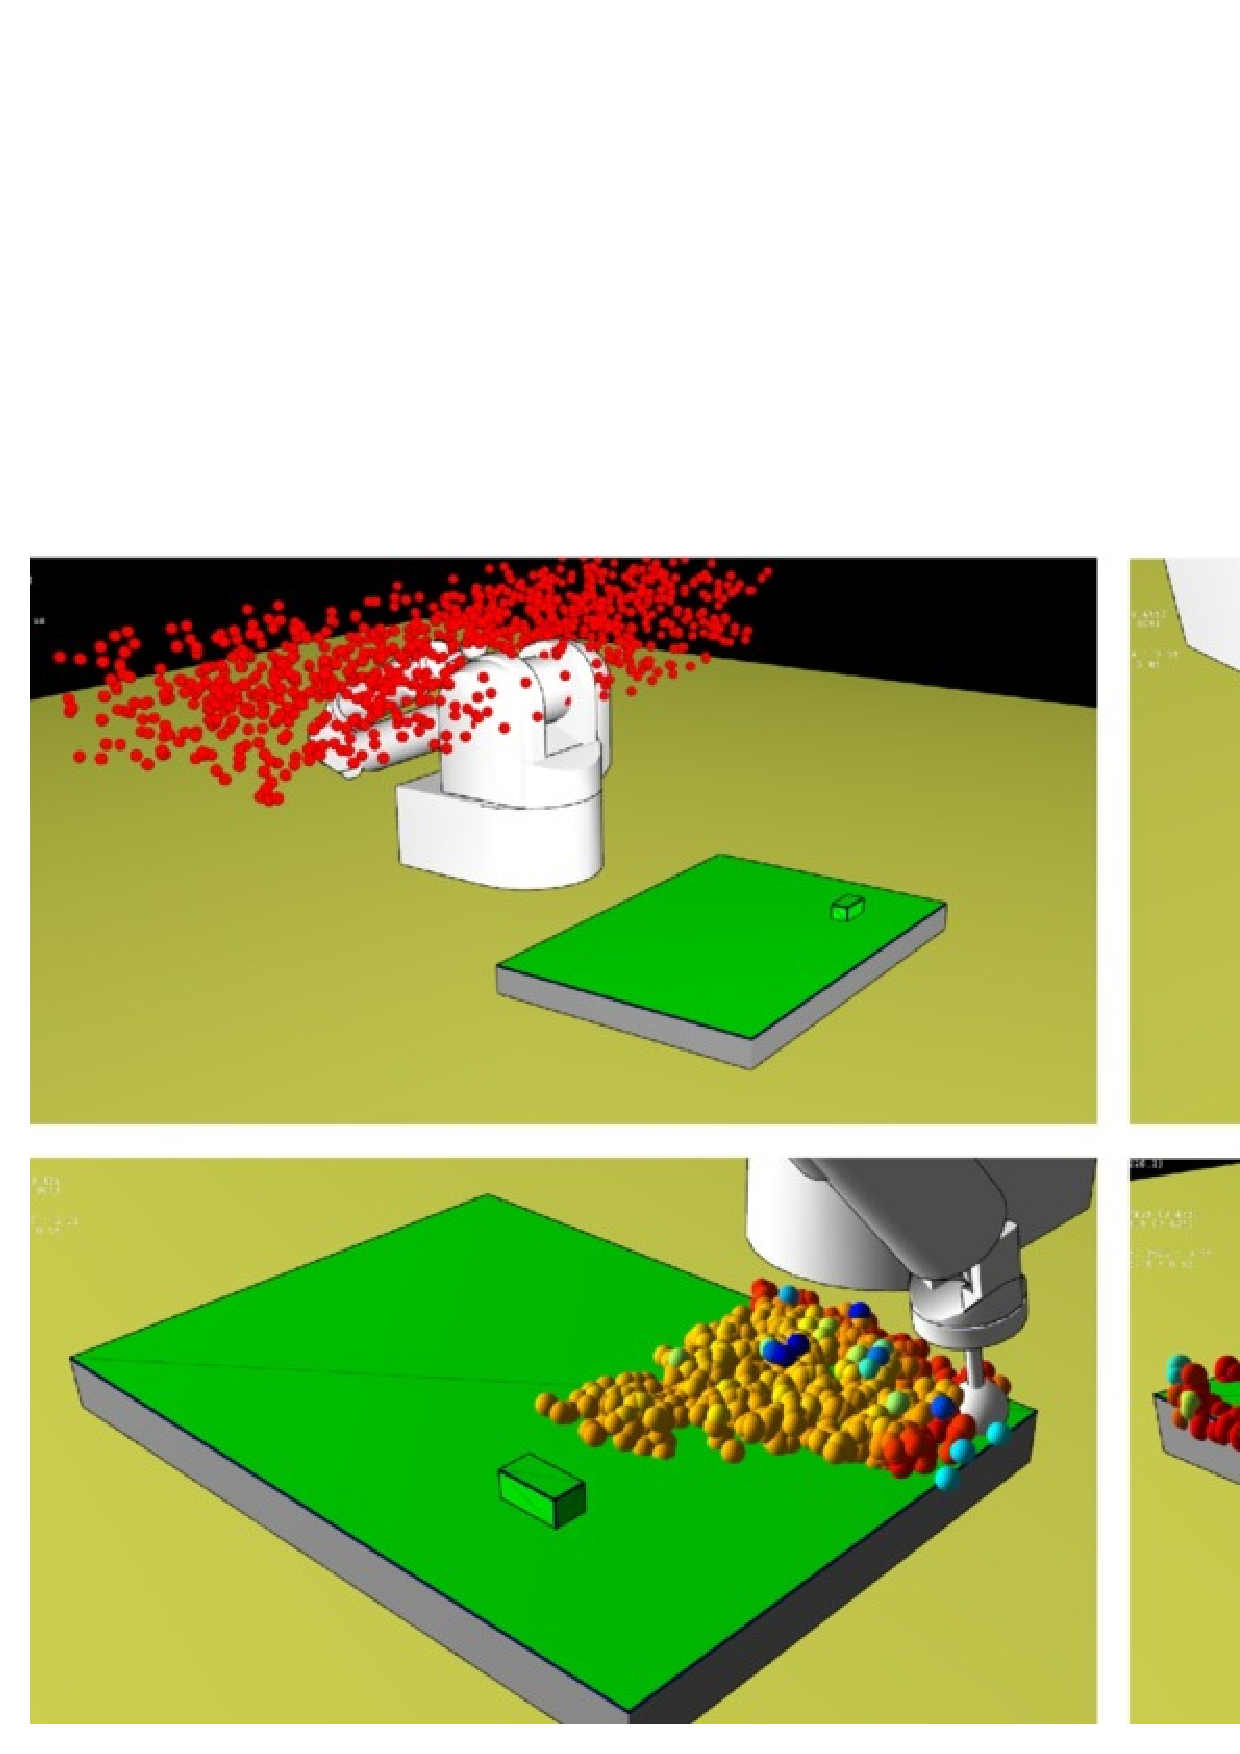
\includegraphics[width=\textwidth]{./ch3-Search/Figures/particlefilter.pdf}
  \caption{Four different time frames of the evolution of the belief particle filter. \textit{Top left}: Initial belief distribution; a lot of uncertainty.
  \textit{Top right:} First contact is made with the table, the measurement likelihood restrains the samples to be on the table's surface. \textit{Bottom right:}
  First contact is an edge. \textit{Bottom left:} Gradual localisation.}
  \label{fig:pf_example}
\end{figure}

\subsubsection{Motion model}

The motion model is straight forward compared with the sensing model. In the robot's case the Jacobian gives the next 
Cartesian position given the current joint angles and angular velocity of the robot's joints.
From this the motion model is given by $ p(x_{t}|x_{t-1},\dot{x}_{t}) = \mathrm{J}(q)\dot{q} + \epsilon$ where $q$ is 
the angular position of the robot's joints, $J(q)$ is the Jacobian and $\epsilon \sim \mathcal{N}(0,\sigma^{2}I)$ is white noise. 
The robot's motion is very precise and its noise variance is very low. For humans, the motion model is the velocity of the hand 
movement provided by the tracking system. In our experiment we consider the noise from motion to be negligible. An increase in 
uncertainty already results from the re-sampling stage of Sampling Importance Resampling (SIR) particle filter and we found 
no need to add additional motion noise.
The particles' positions were updated by applying the measured velocity obtained from either the visual tracking system 
(when recording the human demonstrations) or the robot's forward kinematics.

\subsubsection{Uncertainty}

% First motivate entropy as a natural method for computing the uncertainty

In a probability distribution framework, entropy is used to represent uncertainty. It is the expectation of a 
random variable's total amount of unpredictability. The higher the entropy the more the uncertainty, likewise the 
lower the entropy, the less the uncertainty. In our context, a set of weighted samples $\{w_{i},x_{i}\}^{i=1\dots N}$ replaces 
the true probability density function of the belief, $p_{\Param}(x_t|y_{0:t},\dot{x}_{0:t})$. A reconstruction of 
the underlying probability density is achieved by fitting a Gaussian  Mixture Model (GMM), Equation \ref{eq:gmm1}, to the particles,

\begin{equation}\label{eq:gmm1}
  p_{\Param}(x_t|y_{0:t},\dot{x}_{0:t}) = \sum\limits_{k=1}^{K} \piK\, g(x_t\: ;\MuK,\SigK )
\end{equation}
where parameters $\Param = \{w^{[k]},\MuK,\SigK\}_{1,\dots,K}$, are the weights, means and covariances of the individual multivariate Gaussian function, $g(\cdot)$ and
$K$ is the number of Gaussian components. The scalar $\piK$ represents the weight associated to mixture component $k$ 
(indicating the component's overall contribution to the distribution) and $\sum_{k=1}^{K} \piK = 1$. The parameters $\MuK \in \mathbb{R}^{(3\times 1)}$ 
and $\SigK \in \mathbb{R}^{(3\times 3)}$ are the mean and covariance of the normal distribution $k$. 

The main difficulty here is determining the number of parameters of the density function in a computationally efficient manner.
We approach this problem by finding all the modes in the particle set via mean-shift hill climbing and set these as the 
means of the Gaussian functions. Their covariances are determined by maximizing the likelihood of the density function 
via Expectation-Maximization (EM). 
%
%	images/clustering.eps
%

\begin{figure}
 \centering
   \includegraphics[width=0.95\textwidth]{./ch3-Search/Figures/Figure3}
  \caption{Representation of the estimated density function. \textit{Top Left and Right:} Initial starting point, 
  all Gaussian functions are uniformly distributed with uniform priors. The red cluster always has the highest likelihood which is taken
  to be the believed location of the robot's/human's end-effector. \textit{Bottom Left:} Contact with the table has been established, the robot location differers
  from his belief. \textit{Bottom Right:} Contact has been made with a corner, the clusters reflect that the robot could be at any corner (note that weights are not 
  depicted, only cluster assignment).}
  \label{fig:clustering}
\end{figure}

Given the estimated density we can compute the upper bound of the differential entropy \cite{DiffEntropyHuber2008}, $H$,
%which is taken to be the uncertainty $U$,
\begin{equation}
  H\left(  p_{\Param}(x_t|y_{0:t},\dot{x}_{0:t}) \right) = \sum\limits_{k=1}^{K} \piK\ \left( -\log(\piK) + \frac{1}{2} \log((2\pi e)^{D} |\Sigma_{k}|) \right)
\end{equation}
where $e$ is the base of the natural logarithm and $D$ the dimension (being 3 in our case).

The reason for using the upper bound is that the exact differential entropy of a mixture of Gaussian functions has no 
analytical solution. When computing both the
upper and lower bounds it was found that the difference between the two was insignificant, making any bound a good approximation 
of the true entropy. The choice of the believed location of the robot/human end-effector is taken to be the mean of the 
Gaussian function with the highest weighted $\pi$.

\begin{equation}
 \hat{x}_t = \operatorname*{arg\,max}_{x_t} p_{\Param}(x_{t}|z_{0:t}) = \mu_{(k = \max(w))}
\end{equation}

Figure \ref{fig:clustering} depicts different configurations of the modes (clusters) and believed position of the end-effector (indicated by a yellow arrow).  



%%%%%%%%%%%%%%%%%%%%%%%%%%%%%%%%%%%%%%%%%%%%%%%%%%%%%%%%%%%%%%%%%%%%%%%%%%%%%%%%%%%%%%%%%%%%%%%%%%%%%%%%%%%%%%%%%%%%%%%%%%%%%%%%%%%%%%%%%
%																	   %
%					Methods												   %
%																	   %
%%%%%%%%%%%%%%%%%%%%%%%%%%%%%%%%%%%%%%%%%%%%%%%%%%%%%%%%%%%%%%%%%%%%%%%%%%%%%%%%%%%%%%%%%%%%%%%%%%%%%%%%%%%%%%%%%%%%%%%%%%%%%%%%%%%%%%%%%


\section{Policies}\label{chap3:policies}

\subsection{Modelling human search strategies}\label{chap3:GMM_policy}

During the experiments, the recorded trajectories show that different actions are present for the same belief and uncertainty making the data multi-modal
(for a particular position and uncertainty different velocities are present). That is multiple actions are possible given a specific belief. 
This results in a one-to-many mapping which is not a valid function, eliminating any regression technique which directly learns a non-linear function. 
To accommodate this fact we use a GMM to model the human's demonstrated searches, $\{(x,\dot{x},U)\}$. 
Using statistical models to encode control policies in robotics is quite common, see \cite{Billard08chapter}. 

% explain how much data we have vs the number of gaussian components
By normalising the velocity the amount of information to be learned was reduced. We also took into consideration that velocity is more 
specific to embodiment capabilities: the robot might not be able to reproduce safely some of the velocity profiles demonstrated. 

The training data set comprised a total of 20'000 tuples $(\dot{x},\hat{x},U)$, from the 150 trajectories gathered from the demonstrators. 
The fitted GMM $\pi_{\Param}(\dot{x},\hat{x},U)$ had a total of 7 dimensions, 3 for direction, 3 for position and 1 scalar for uncertainty. 
The definition of the GMM is presented below in equation \ref{eq:gmm2}.

\begin{equation} \label{eq:gmm2}
 \pi_{\Param}(\dot{x},\hat{x},U) = \sum\limits_{k=1}^{K} \piK\, g(\dot{x},\hat{x},U\: ;\MuK,\SigK )
\end{equation}

\begin{equation*}
    \MuK =
    \begin{bmatrix}
      \mu_{\dot{x}} \\
      \mu_{\hat{x}} \\
      \mu_{U}
    \end{bmatrix}
    \SigK =
    \begin{bmatrix}
      \Sigma_{\dot{x}\dot{x}} & \Sigma_{\dot{x}\hat{x}} & \Sigma_{\dot{x}U} \\
      \Sigma_{\hat{x}\dot{x}} & \Sigma_{\hat{x}\hat{x}} & \Sigma_{\hat{x}U} \\
      \Sigma_{U\dot{x}} & \Sigma_{U\hat{x}} & \Sigma_{UU}   
    \end{bmatrix}
\end{equation*}
Given this generative representation of the humans' demonstrated searches we proceeded to 
select the necessary parameters to correctly represent the data. This step
is know as model selection and we used Bayesian Information Criterion (BIC) to evaluate
each set of parameters which were optimised via Expectation-Maximisation (EM). 

A total of 83 Gaussian functions were used in the final model, 67 for trajectories on the table and 15 for those in the air. In Figure
\ref{fig:gmm} \textit{(left)} we illustrate the model learned from human demonstrations where we plot the 3 dimensional slice (the position) of the 7
dimensional GMM to give a sense of the size of the model.

\begin{figure}
\centering
  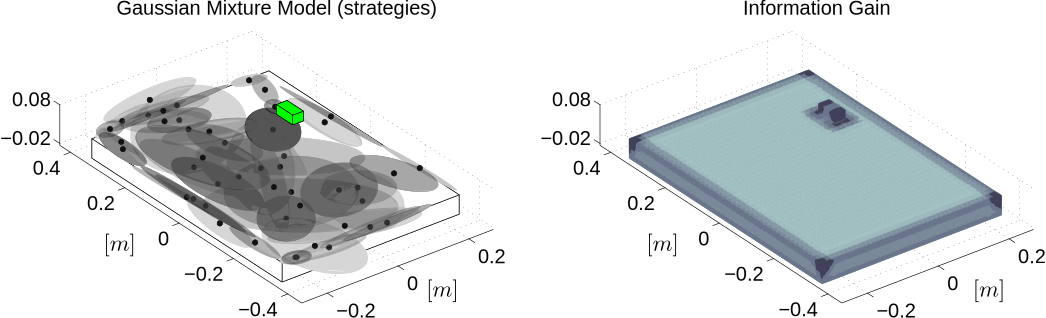
\includegraphics[width=0.95\textwidth]{./ch3-Search/Figures/Figure4}
  \caption{\textit{Left: } Resulting search GMM, a total of 67 Gaussian mixture components are present. We note the many overlapping Gaussians: this results
from the level of uncertainty over the different choices taken. For example humans follow along the edge of the table in different directions and might
leave the edge once they are confident with respect to their location. \textit{Right:} Information Gain map of the table environment, dark regions indicate 
high information gain as oppose to lighter ones. Not surprisingly, the highest are the corners, followed by the edges.}
  \label{fig:gmm}
\end{figure}

\subsection{Coastal Navigation}\label{chap3:costal_policy}

Coastal navigation \cite{CostalNavigation1999} is a path planning method in which the objective function, 
Equation \ref{eq:objective_function}, is composed of two terms.

\begin{equation}\label{eq:objective_function}
 f(x_{0:T}) = \sum\limits_{t=0}^{T} \lambda_1 \cdot c(x_t) + \lambda_2 \cdot I(x_t)
\end{equation}

The first term, $c(x_t)$, is the traditional ``cost to go'' which penalizes every step taken so as to ensure that the
optimal path is the shortest. The value was simply set to 1 for all discrete states in our case. The second term, $I(x_t)$, 
is the information gain of a state. The information gain, $I$, of a particular state is related to how much 
the entropy of a probability density function (pdf), being the location's uncertainty in our case, can be reduced. The two $\lambda$'s are scalars which weigh the influence 
of each term.

In our table environment we discretised the state space, $\mathbb{R}^3$, into bins so as to have a resolution of approximately, $1 cm^3$, giving us a total of a 125'000
states. The action space was discretised to 6 actions, two for each dimension meaning that all motion is parallel to the axis. For each state, $x_t$, an $I(x_t)$ value is
computed by evaluating Equation \ref{eq:IG},

% Explain how the Information Gain is computed

\begin{equation}\label{eq:IG}
 I(x_t) = \mathbb{E}_{p(y_t|x_t)}\{ H(p_{\Param}(x_t|y_{0:t},\dot{x}_{0:t}) \} - H(p_{\Param}(x_t|y_{0:t-1},\dot{x}_{0:t}))
\end{equation}
which is essentially the difference between the entropy of a prior pdf to that of a posterior pdf.
We set our initial pdf to be uniformly distributed and  we computed the maximum likelihood sensation for each discrete state $x_t$
which is akin to the expected sensation or assuming that there is no uncertainty in sensor measurement (an assumption 
often made throughout the literature to avoid carrying out the integral of the expectation in Equation \ref{eq:IG}).
The result is the difference between the posterior pdf, given that the sensation occurred in $x_t$, and the prior pdf. The resulting cost
map is illustrated in Figure \ref{fig:gmm}. As expected, corners have the highest information gain followed by edges and surfaces. 
We do not show the values of the table since they provided much less information gain.

The optimization of the objective function is accomplished by running the Dijkstra's algorithm. This algorithm, given a cost map, 
computes the shortest path to a specific target from all the states. This results in a policy.

\subsection{Control}
The standard approach to control with a GMM is to condition on the state,
$\hat{x}_t$ and $U_t$ in our case, and perform inference on the resulting conditional
GMM, Equation \ref{eq:conditional}, which is a distribution over velocities or directions.

\begin{equation} \label{eq:conditional}
  \pi_{\Param}(\dot{x}|\hat{x},U) = \sum\limits_{k=1}^{K} w^{k}_{\dot{x}|\hat{x},U} \;\;  g\left(\dot{x}\: ;  \MuK_{\dot{x}|\hat{x},U}, \SigK_{\dot{x}|\hat{x},U} \right)
\end{equation}

The new distribution is of the dimension of the output variable, the velocity (dimension 3). 
The variable $\dot{x}$ in $\dot{x}|\hat{x},U$ indicates the predictor variable and the variables $\hat{x},U$ have been conditioned.
A common approach in statistical PbD methods using GMMs is to take the expectation of the conditional (known as Gaussian Mixture Regression), equation \ref{eq:GMR}

\begin{equation} \label{eq:GMR}
 \dot{x} = \mathbb{E}\{\pi_{\Param}(\dot{x}|\hat{x},U)\} = \sum\limits_{k=1}^{K}  w^{[k]}_{\dot{x}|\hat{x},U} \; \MuK_{\dot{x}|\hat{x},U}
\end{equation}

The problem with this expectation approach, is that it averages out opposing directions or strategies and may leave 
a net velocity of zero. One possibility would be to sample from the conditional, however this can lead to non-smooth 
behaviour and flipping back and forth between modes resulting in no displacement. To maintain consistency between the
choices and avoid random switching  we perform a weighted expectation on the means so that 
directions (modes) similar to the current direction of the end-effector receive
a higher weight than opposing directions. For every mixture component $k$, a weight $\alpha_k$ is computed based 
on the distance between the current direction and itself.
If the current direction agrees with the mode then the weight remains unchanged but if it is in
disagreement a lower weight is
calculated according to the equation below. 
\begin{equation}  \label{eq:weight}
  \alpha_{k}(\dot{x}) = \piK_{\dot{x}|\hat{x},U} \; \exp(-\cos^{-1}(<\dot{x},\MuK_{\dot{x}|\hat{x},U}>))
\end{equation}
Gaussian Mixture Regression is then performed with the normalised  weights $\alpha$ instead of $\pi$
(the initial weight obtained when conditioning).

\begin{equation}\label{eq:w_expectation}
 \dot{x} = \mathbb{E}_{\alpha}\{\pi_{\Param}(\dot{x}|\hat{x},U)\} = \sum\limits_{k=1}^{K} \alpha_{k}(\dot{x}) \:\MuK_{\dot{x}|\hat{x},u}
\end{equation}
% 
%	How to control speed
%
The final output of equation \ref{eq:w_expectation} gives the desired direction
($\dot{x}$ is re-normalised). In the case when the mode suddenly disappears
(because of sudden change of the level of uncertainty caused by the appearance or disappearance of a feature)
another present mode is selected at random. For example, when the robot has reached a corner, the level of uncertainty for this feature drops to zero.
A new mode, and hence new direction of motion, will then  be computed.
However this is not enough to be able to safely control the robot.
One needs to control the amplitude of the velocity and ensure compliant control 
of the end-effector when in contact with the table. This behaviour is not learned here, as this is specific to 
the embodiment of the robot and unrelated to the search strategy. The 
amplitude of the velocity is computed by a proportional controller based on the
believed distance to the goal,
\begin{equation}
 \nu = \max(\min(\beta_{1},K_{p}(x_{\mathrm{g}} - \hat{x}),\beta_{2})
\end{equation}
where the $\beta$'s are lower and upper amplitude limits, $x_{g}$ is the
position of the goal, and $K_{p}$ the proportional gain which was tuned through
trials.

%
%	images/flow_chart.eps
%

\begin{figure}
\centering
  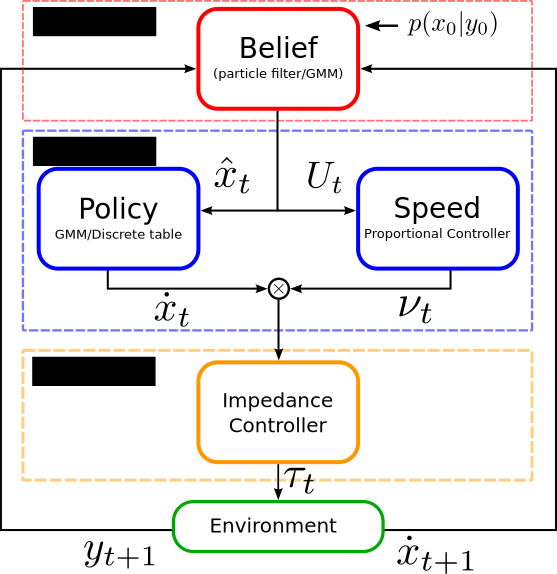
\includegraphics[width=0.8\textwidth]{./ch3-Search/Figures/Control_schematics}
  \caption{Overview of the decision loop. At the top a strategy is chosen given an initial belief
$p(x_{0}|y_{0})$ of the location of the end-effector (initially through sampling the conditional). 
A speed is applied to the given direction based on the believed distance
to the goal. This velocity is passed onwards to
a low level impedance controller which sends out the required torques. The
resulting sensation, encoded through the Multinomial distribution over
  the environment features, and actual displacement are sent back to update the
belief.}
  \label{fig:flow_chart}
\end{figure}

%
%	Impedance controller
%
As mentioned previously, compliance is the other important aspect when having the robot duplicate the search strategies. 
Collisions with the environment occur as a result of the uncertainty. To avoid risks of breaking the table or the robot sensors we have an impedance controller
at the lowest level which outputs appropriate joint torques $\tau$. The overall control loop is depicted in Figure \ref{fig:flow_chart}.



%%%%%%%%%%%%%%%%%%%%%%%%%%%%%%%%%%%%%%%%%%%%%%%%%%%%%%%%%%%%%%%%%%%%%%%%%%%%%%%%%%%%%%%%%%%%%%%%%%%%%%%%%%%%%%%%%%%%%%%%%%%%%%%%%%%%%%%%%
%																	   %
%				Results and Discussion  										   %
%																	   %
%%%%%%%%%%%%%%%%%%%%%%%%%%%%%%%%%%%%%%%%%%%%%%%%%%%%%%%%%%%%%%%%%%%%%%%%%%%%%%%%%%%%%%%%%%%%%%%%%%%%%%%%%%%%%%%%%%%%%%%%%%%%%%%%%%%%%%%%%
\FloatBarrier
\section{Results and discussion}\label{chap3:results}

Throughout our evaluation of our GMM PbD-POMDP control policy we will be considering four search policies: Greedy, GMM, Hybrid and 
Coastal. We evaluate behaviour present in the human demonstrations, and the four above mentioned policies in terms 
of their riskiness. We qualitatively compare the policies of the GMM model and the Coastal Navigation algorithm and highlight the 
effect of uncertainty. We finish with a quantitative evaluation of search efficiency in terms of distance travelled until the goal is found.
The layout of this section follows as:
\begin{itemize}
 \item Section \ref{sub:search_behaviour}, we analyse the types of behaviour present in the human demonstration as well as in
four different search algorithms: Greedy, GMM, Hybrid and Coastal.
 \item Section \ref{sub:policy_analysis}, we qualitatively analyse the GMM search policy (namely the different modes/decisions present) 
 with respect to the Coastal navigation policy.
 \item Section \ref{sub:time_uncertainty}, we evaluate the search performance, with respect to the distance taken to reach the goal and the uncertainty profiles towards the end of 
the searches in 5 different experiments (different types of initializations). 
\end{itemize}
\FloatBarrier
\subsection{Search \& behaviour analysis}\label{sub:search_behaviour}

For each method (Greedy, GMM, Hybrid, Coastal) 70 searches were performed with all starting positions drawn from the
uniform distribution used during the teaching stage (depicted in Figure \ref{fig:experiment} \textit{top right}, page \pageref{fig:experiment}). 
In Figure \ref{fig:expectedfeatures} we illustrate the expected sensation $\mathbb{E}\{y\}$ and  variance $\mathrm{Var}\{y\}$ for each trajectory with respect 
to the edge and corner of the table. 

\begin{figure}
  \centering
  \includegraphics[width=\textwidth]{./ch3-Search/Figures/Figure6} 
  \caption{Expected sensation. Plots of the expected sensation of the edge and corner feature for all trajectories. 
  The axes are associated with the 
  sensor measurements, 0 means that the corresponding feature is not sensed and 1 the feature is fully sensed. 
  A point in the plots summarises a whole trajectory by the mean and variance of the probability of sensing a corner or edge. 
  The radius of the circles are proportional to the variance. The doted blue rectangle represents the decision boundary 
  for classifying a trajectory as being either risk-prone or risk-averse. A point which lies inside the rectangle is risk-prone.
  \textit{Left:} Human trajectories demonstrate a wide variety of behaviours ranging from those remaining close to features 
  to those preferring more risk. 
  \textit{Right:} Red points show Greedy and blue points the GMM model. 
  \textit{Bottom:} Green circles are associated with the Hybrid method whilst orange are those of the 
  Coastal navigation method. The Hybrid method is a skewed version of the GMM which tends towards risky behaviour and exhibits the 
  same kind of behaviour as the Coastal algorithm.}
  \label{fig:expectedfeatures}
\end{figure}


The selection of edges and corners as features as a means of classifying the type of behaviours present 
is not solely restricted to our search task. Salient landmarks will result in a high level of information
gain, which is the case for the edge and corner (see Figure \ref{fig:gmm} \textit{right}, page \pageref{fig:gmm}).
Other tasks can use such features or variants in which the curvature is considered for representing the task space. 
These features are present in most settings and high level features can use these easily as their building blocks.

We note that the Greedy search approach seeks to go directly to the goal without taking into account 
the uncertainty. The GMM models human search strategies. The Hybrid is a combination of both the Greedy and GMM method 
where once the uncertainty has been sufficiently minimised, the policy switches (threshold) to the Greedy method for the rest of 
the search. The Coastal navigation algorithm finds the optimal path to the goal based on an objective function which
consists of a trade-off between time taken to reach the goal and the minimisation of the uncertainty.

It can be seen that the human demonstrations have a much wider spread than those of the search algorithms. 
We suggest that this is due to human behaviours being optimal with respect to their own criteria as opposed to the algorithms 
which usually tend to only maximise a single objective function. The trajectories of the Greedy and GMM methods represented by their 
expected features demonstrate two distinctive behaviours (in terms of expected sensation), risk-prone for the Greedy and risk-adverse
for the GMM.

We make \textbf{the assumption} that Greedy trajectories are risk-prone by nature. We performed a SVM classification on the 
Greedy-GMM expected features (Figure \ref{fig:expectedfeatures} \textit{right}) and used the result to construct a decision boundary as a means
of classifying a trajectory as being either risk-prone or risk-averse. Table \ref{tab:percentage-risk-prone} \textit{first row} shows that
the GMM and Human search trajectories are mostly risk-averse. Surprisingly the Coastal policy seems to be very risk-prone given 
that it seeks paths close to highly informative areas.
We use a second metric based on the information gain, which we call the Risk factor, to classify trajectories as being either 
risk-prone or risk-averse.

The Risk factor of each individual trajectory is inversely proportional to its accumulated information gain. Figure \ref{fig:riskexamples} (\textit{left}) shows the kernel density estimation distribution of the risk 
for each search method. Two trajectories per search type corresponding to a supposed risk-prone and risk-averse search
are plotted in the expected feature space in Figure \ref{fig:riskexamples} (\textit{right}). As expected, risk-prone strategies 
for which the risk tends to 1 have a low expectation of sensing edges and corners and produce trajectories with a 
low information gain while those with a high expectation of sensing features have a high information gain. 
Since the metric lies exclusively in the range [0,1] we define that every trajectory which has a Risk factor lower than than 0.5 will 
be considered risk-averse whilst those above are risk-prone. Table \ref{tab:percentage-risk-prone} \textit{second row} illustrates
the riskiness of each search method. It is evident that humans are risk-averse in general followed by GMM which is a smoothing 
of the human data, then Hybrid which as expected should be more risk-prone since it is a linear interpolation between the GMM and 
Greedy search policies and finally Coastal and Greedy.

\begin{figure}
  \centering
  \includegraphics[width=\textwidth]{./ch3-Search/Figures/Figure7} 
 \caption{Risk of searches. Illustration of risk-prone and risk-averse searches in terms of a Risk factor (\textit{left}) and expected sensation (\textit{right}).
 \textit{Left:} Each trajectory was reduced to a single scalar, which we call the Risk factor, quantifying the risk of a trajectory. The Risk factor 
 is inversely proportional to the sum of the information gain of a particular trajectory. The colour paired dots (risk averse) and squares (risk prone) 
 represent trajectories which are plotted in 
 Figure \ref{fig:risk_examples}, to illustrate that these correspond to risk averse and prone searches.
 \textit{Right:} Corresponding trajectories chosen in the Risk factor space but represented in the feature space. As expected, trajectories with
 a high risk map to regions of low expected feature. However the transition from the Risk space to feature space is non-linear and will result in a different
 risk-level classification than the feature metric previously discussed.}
 \label{fig:riskexamples}
\end{figure}



\begin{table}
\centering
\begin{minipage}{\textwidth}
\centering
 \begin{tabular}{|l|c|c|c|c|c|}
 \cline{1-6}
   Criteria        &  \textbf{Greedy} & \textbf{GMM}  & \textbf{Hybrid} & \textbf{Coastal} & \textbf{Human} \\ \hline
  risk-prone (f) &   77 \% & 11 \% &  30 \% & 46 \% & 26  \% \\ \hline
  risk-prone (r) &   78 \% & 12 \% &  24 \% & 45 \% &  7 \% \\ \hline
 \end{tabular}
\end{minipage}
 \caption{Percentage of risk-prone trajectories based on two decision criteria, the feature (f) and the risk (r) (information gain) metrics discussed above.}
 \label{tab:percentage-risk-prone}
\end{table}

Figure \ref{fig:risk_examples} (\textit{top left \& right}), shows risk-prone (red) and 
averse (green) trajectories produced by human demonstrations and by the Greedy search. Both these extremes
correspond to our intuition that risk-averse trajectories tend to remain closer to features or areas of high information gain
as oppose to risk-prone searches. However to stress the case that humans have multiple search strategies 
present, we performed 40 GMM searches (model of the human behaviour) which all started under the same initial conditions
(same belief distribution, true position and believed position). Figure \ref{fig:risk_examples}
shows the resulting trajectories and expected features for each trajectory. 
It is clear that multiple searches occur which is reflected in the plot of the expected features. All of the 
search strategies generated by the GMM for this initial condition produced risk-averse trajectories.


We conclude that there is a strong inclination towards inferring that indeed multiple search strategies do 
arise in the human searches since they were extracted and encoded in the GMM model. From the risk distribution, humans have a 
tendency to be risk-averse.

\begin{figure}
 \centering
  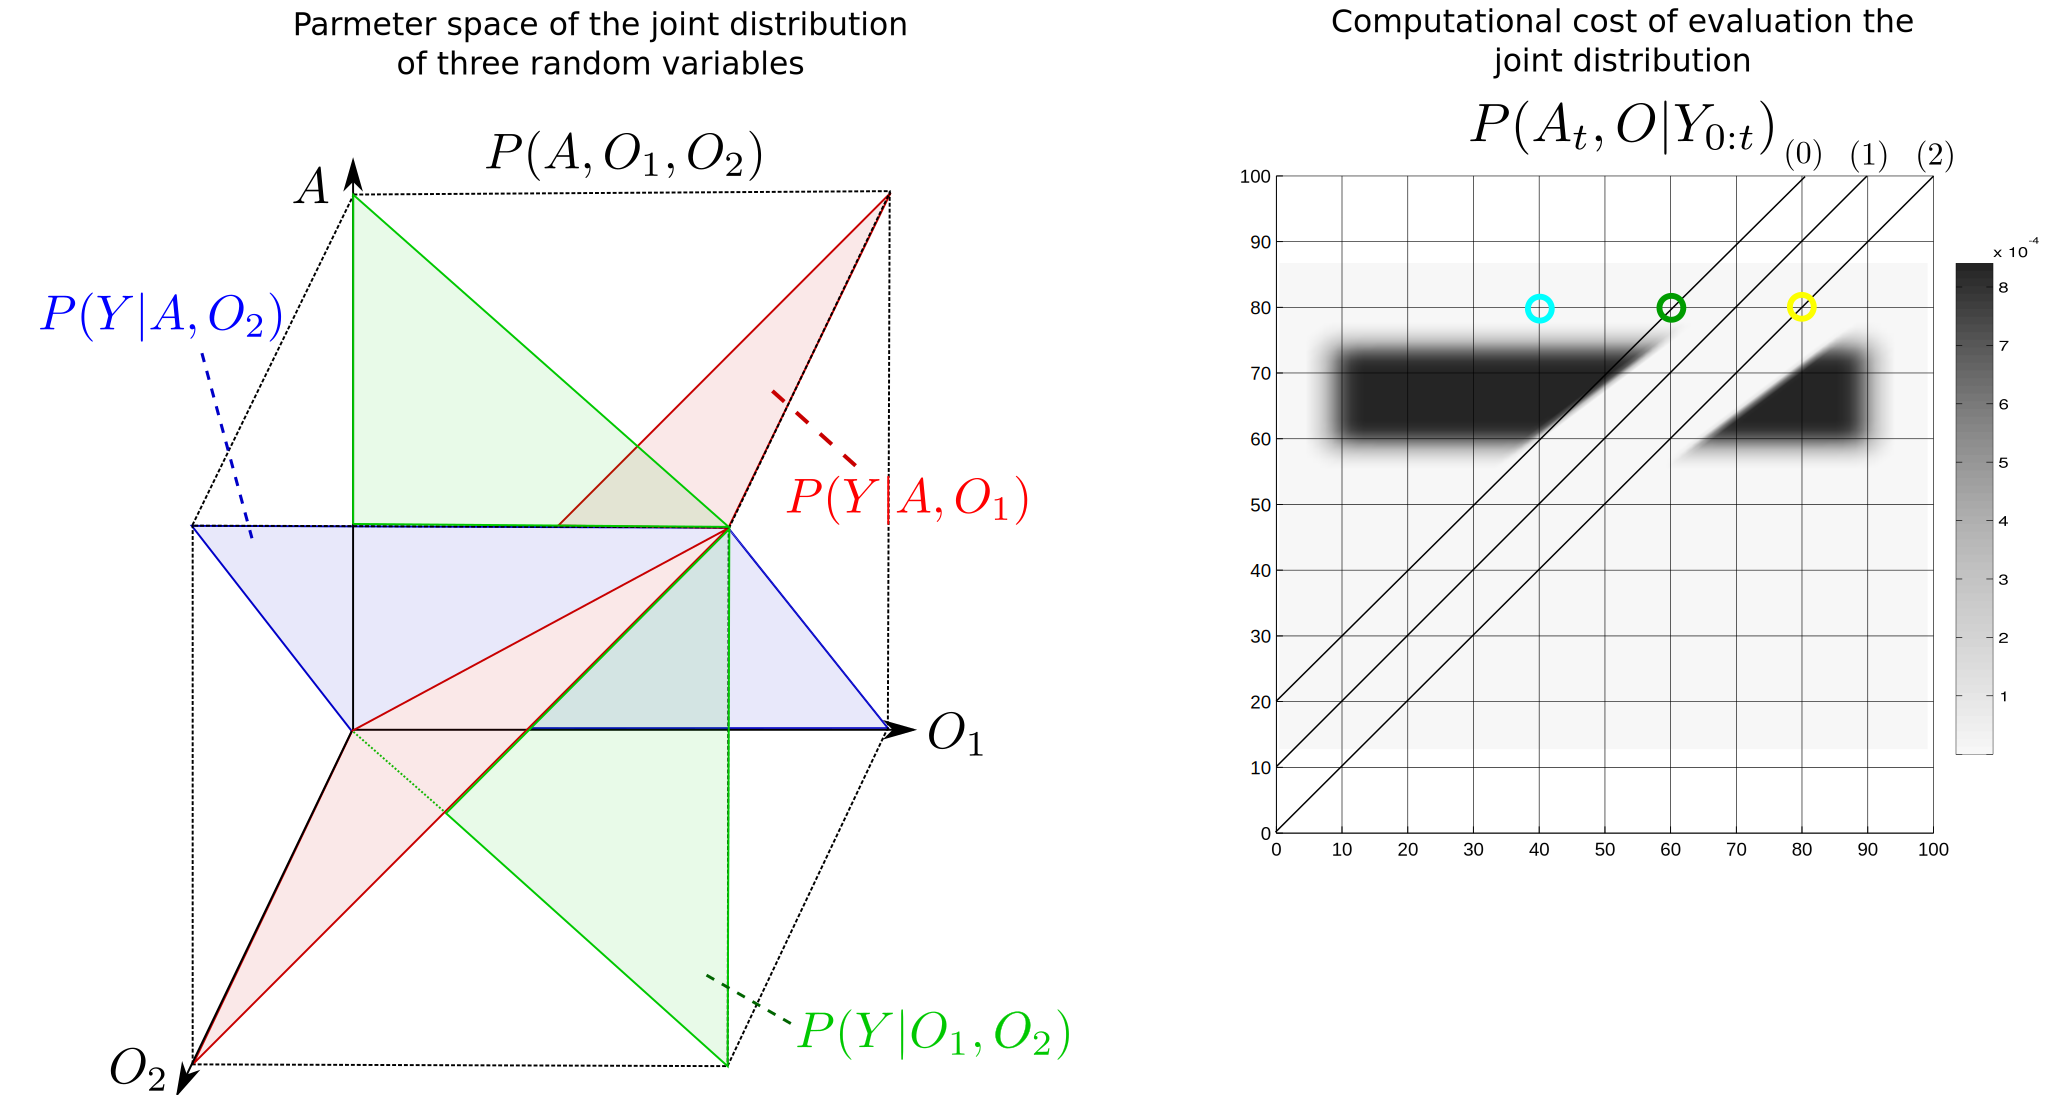
\includegraphics[width=0.95\textwidth]{./ch3-Search/Figures/Figure8}
  \caption{Risk prone \& averse searches (red \& green trajectories). \textit{Top left:}
  Two human trajectories taken from data shown in Figure \ref{fig:riskexamples}. 
  \textit{Top right:} Two Greedy trajectories. \textit{Bottom left:} GMM trajectories, all starting from the same location, the
  colour coding is to illustrate the different policies which were encoded and emerge given the same initial conditions. 
  \textit{Bottom right:} Corresponding expected features of each trajectory, the colour coding matches the trajectories 
  to the ``GMM risk types'' sub-figure. All the searches which were generated by the GMM for this initialisation produced
  risk-averse searches (based on the feature metric discussed previous).}
  \label{fig:risk_examples}
\end{figure}

\FloatBarrier
\subsection{GMM \& Coastal Navigation policy analysis}\label{sub:policy_analysis}

We next illustrate some of the modes (action choices) present during simulation and evaluate their 
plausibility. Figure \ref{fig:modes} shows that multiple decision points have been correctly embedded in the GMM model. All
arrows (red) indicate directions that reduce the level of uncertainty. 

\begin{figure}
    \centering
    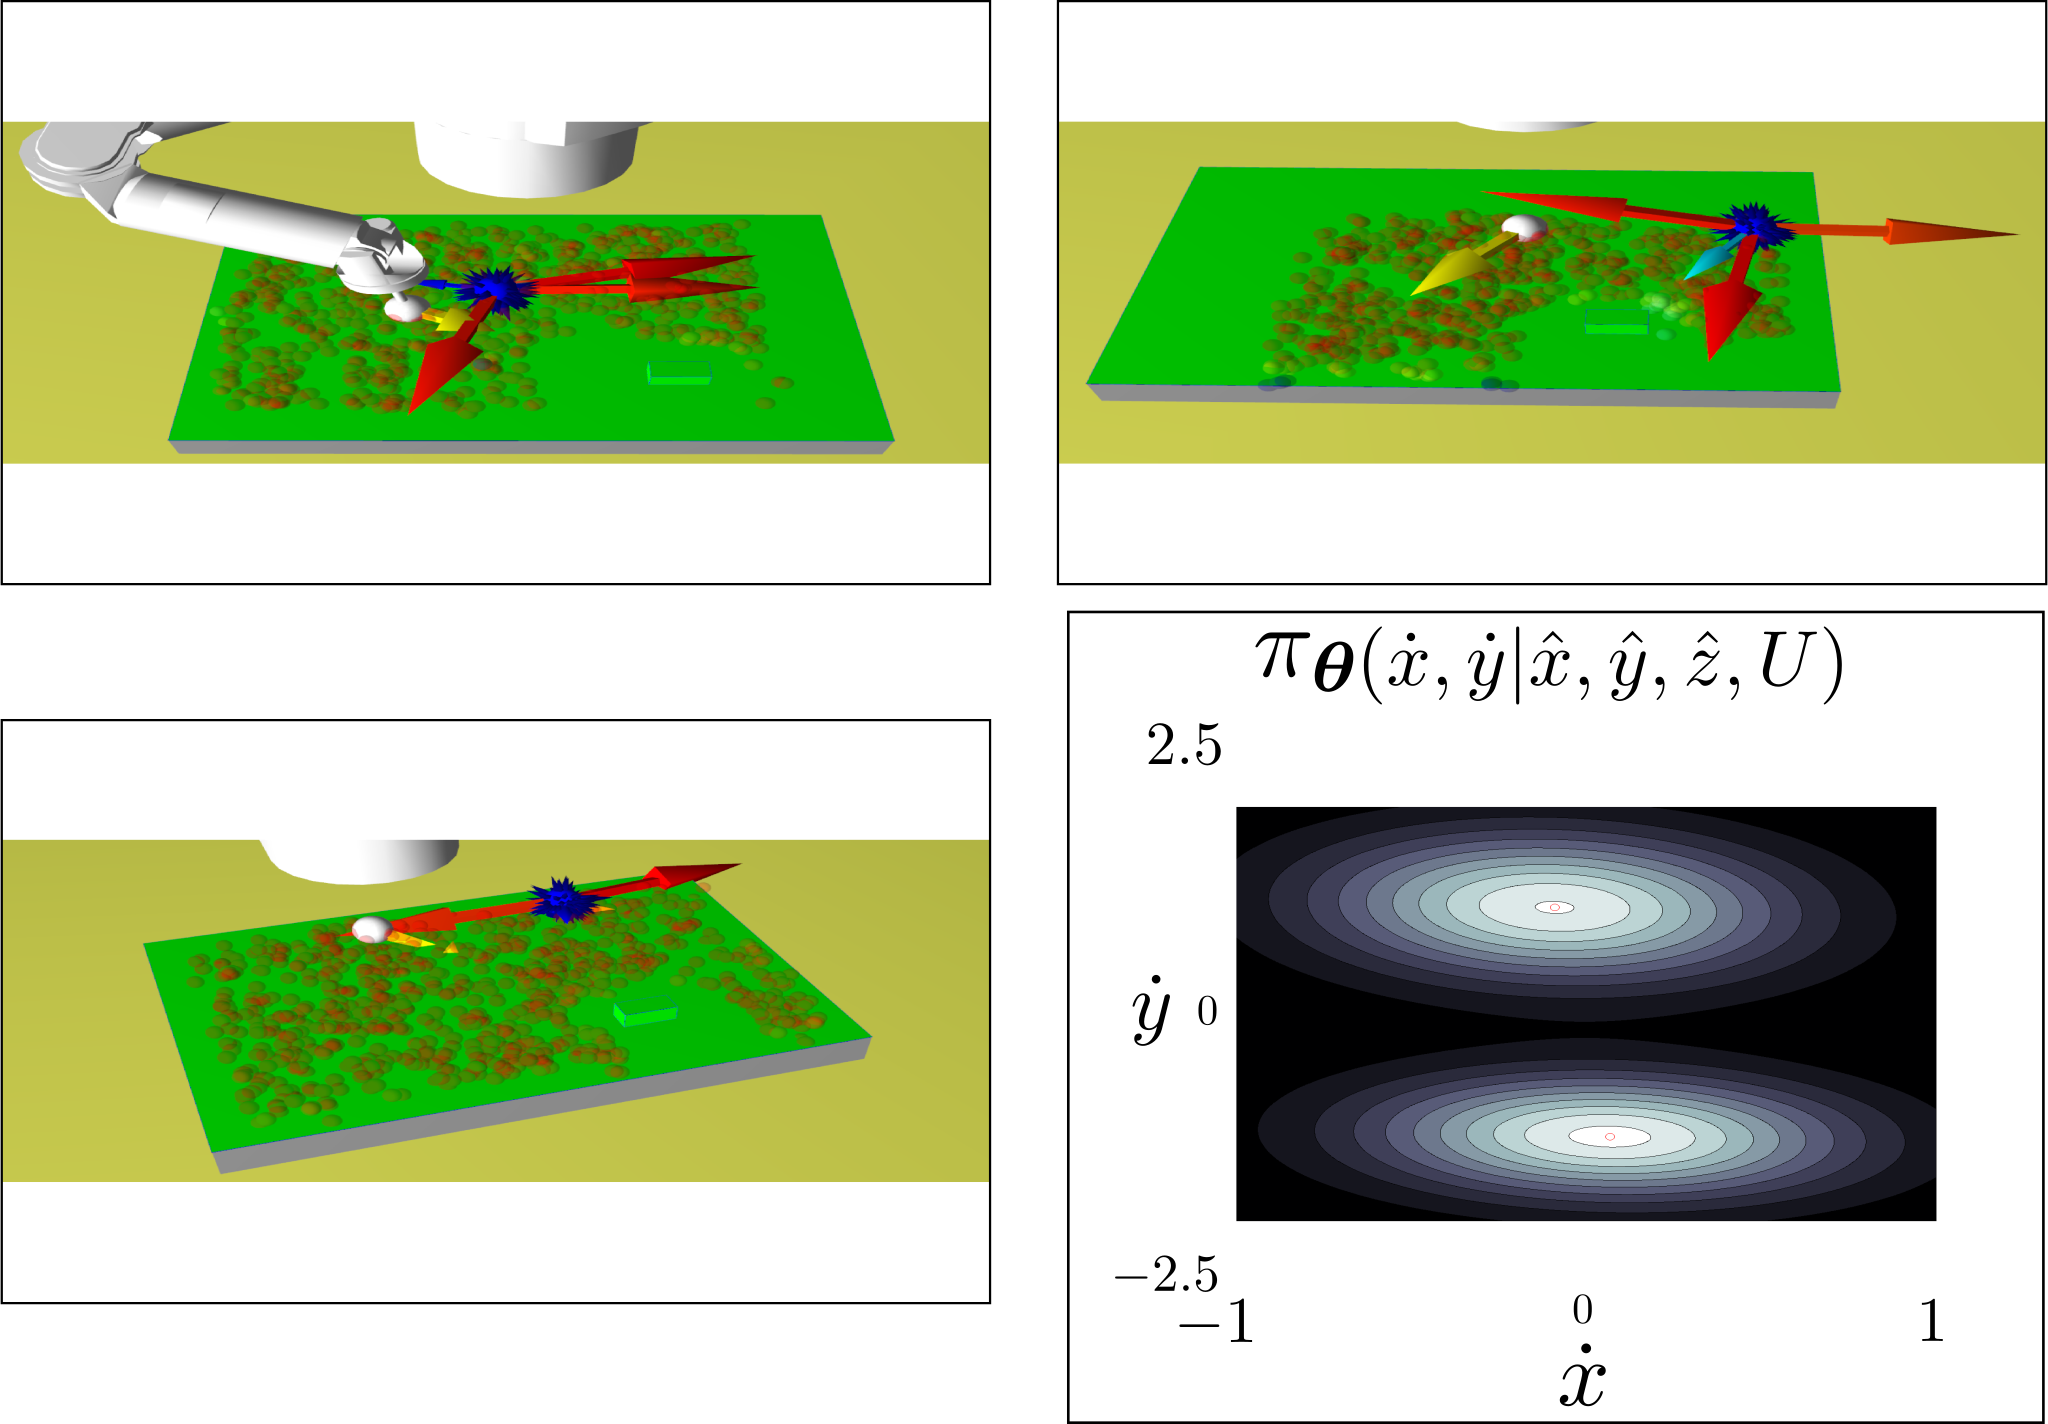
\includegraphics[width=0.95\textwidth]{./ch3-Search/Figures/Figure9_m}
    \caption{Illustration of three different types of modes present during the
    execution of the task where the robot is being controlled by the learned GMM model.
    The white ball represents the actual position of the robot's end-effector. The blue ball represents the
    believed position of the robot's end-effector and the robot is acting according to it. 
    The blue ball arrows represent modes. Colours encode the mode's weights given by the priors $\pi_{k}$ after conditioning ( but not re-weighted as
    previously described). The spectrum ranges from red (high weight) to blue (low weight). \textit{Top left:} Three modes are present, but two agree with each other.   
    \textit{Top right:} Three modes are again present indicating appropriate ways to reduce the uncertainty. \textit{Lower left:} Two modes are in opposing directions. 
    No flipping behaviour between modes occurs since preference is given to the modes pointing in the same direction as the robot's current trajectory. \textit{Lower right:} GMM modes when conditioned on the state represented in the lower left figure.
    The two modes represent the possible directions (un-normalised).}
   \label{fig:modes}
\end{figure}

Figure \ref{fig:vectorfield} depicts the vector fields of both Coastal and GMM models where, as expected, the Coastal navigation 
trajectories tend to stay close to edges and corners until they are sufficiently close to the goal. This is achieved by weighting 
the information gain term $I(x_t)$ in the objective function sufficiently ($\lambda_2$). If $\lambda_2$=0 the Coastal policy is 
the same Greedy algorithm. 

It can be further seen that when the uncertainty tends towards it's maximum value ($U \rightarrow 1$) 
all behaviour tends to go towards the edges and corners. As the uncertainty reduces ($U \rightarrow 0$) the vector field 
tends directly towards the goal. However even at a low level of uncertainty, the behaviour at the edges and corners remains 
multi-modal and tends to favour remaining close to the edges and corners. 
This is an advantage of the GMM model. If the uncertainty has been sufficiently reduced and 
the true position of the end-effector or hand is not near an 
edge the policy dictates to go straight to the goal. This is not the case for the Coastal algorithm which ignores the 
uncertainty and strives to remain in the proximity of corners and edges until sufficiently close. 
This approach could potentially lead to unnecessary travel cost which could otherwise have been avoided.

\begin{figure}
  \centering
  \includegraphics[width=0.95\textwidth]{./ch3-Search/Figures/Figure10}
  \caption{Illustration of the vector field for the Coastal and GMM policy. \textit{Top Left} Coastal policy, there is only one possible direction for every 
  state at any time, the values of $\lambda_2$ in the cost function were set experimentally. \textit{Others:} The GMM policy for three different levels of
  uncertainty. For each point multiple actions are possible which is reflected by the number of arrows (only the first three most likely actions). As 
  the uncertainty decreases the policy becomes less multi-model, but remains around the edges and corners. Note that once certain
  of being close to an edge there is a possibility to go either straight to the goal or stay close to the edge and corners.}
  \label{fig:vectorfield}
\end{figure}

\FloatBarrier
\subsection{Distance efficiency \& Uncertainty}\label{sub:time_uncertainty}

We seek to distinguish the most efficient method in terms of two metrics, the distance (in meters) taken to reach the goal
and the level of uncertainty upon arriving at the goal. We report results on 5 different search 
experiments in which we compare the Greedy, GMM and Coastal Navigation algorithms. The Hybrid was not fully considered since it 
is a heuristic combination of the Greedy and GMM methods. 

In the first experiment, the true and believed locations of the end-effector 
were drawn uniformly from the original start distribution (Figure \ref{fig:experiment}, \textit{top right}) 
reflecting the default setting. The initializations (both real and believed end-effector locations) for the 
remaining 4 experiments were chosen in order to reflect particular situations which highlight the differences 
and drawbacks between each respective search method.
For the first experiment (Uniform search experiment), a 100 trials were carried out in which the end-effector position and belief were 
initialized uniformly. As for the other 4 search experiments, 40 separate runs were carried for each of the three algorithms.

\begin{figure}
   \centering
 \includegraphics[width=\textwidth]{./ch3-Search/Figures/Figure11}
\caption{Four search initializations, from \textit{top left} to \textit{bottom right} we refer to them as \#1-4. The 
circle indicates the true starting point of the end-effector (eof), whilst the triangle is the initial believed location of the eof.
The initialisation in \#1 was chosen such that the true and believed eof locations were at opposite sides of the table. 
This setting was selected to highlight the draw back in methods which do not take into account uncertainty. 
The second initialisation \#2, reflects the situation where once again there is a large distance between true and believed location of 
the eof. However this time both are above the table. The starting points in \#3 are a variant on \#1 
with the difference being that the believed eof position is above the table whilst the true eof location is not. The last 
experiment \#4 was a setup which would be favourable to algorithms that are inclined to be greedy. Both true and believed 
eof locations are close to one another.}
\label{fig:four-initialisations}
\end{figure}

Table \ref{tab:mean-var-distance} reports the mean and variance of the distance taken (in meters) to reach the goal for each search 
method for all 5 experiments.
We report on an Analysis of Variance (ANOVA) to test that all experiments were 
significantly different from one another as were the searches. We test the null hypothesis,  $H_o$,  that there is 
no statistical difference between the 5 search experiments. 
Before performing the ANOVA, we verified that our dependent variable, distance [m] taken to reach the goal, follows a normal 
distribution for all methods and all experiments (a total of $5 \times 3 = 15$ tests), an assumption which is required by 
an ANOVA analysis. A Kolmogorov-Smirnov test was performed on each experiment and associated search method. A total 
of 11/15 searches rejected the null hypothesis with a significance level of less than 5\% (p-value $<$ 0.05). 

\begin{table}
 \centering
  \begin{tabular}{|c|c|c|c|c|}     
  \hline
      Experiment       &  \textbf{Greedy}      	  	&  \textbf{GMM}      		&  \textbf{Coastal}     \\\hline
       Uniform         &   1.54 (0.46) 	  		& 0.99 (0.14) \cellcolor{Gray} 	& 1.13 (0.57)    \\
	\#1            &   3.02 (0.36)    		& 1.82 (0.23) \cellcolor{Gray} 	& 3.44 (1.50)    \\
	\#2            &   0.80 (0.01) \cellcolor{Gray} & 1.41 (0.14) 			& 0.94 (0.01)    \\
	\#3            &   1.14 (0.08) \cellcolor{Gray} & 1.80 (0.17) 			& 2.14 (0.81)    \\
	\#4            &   0.75 (0.04)  		& 1.34 (0.07) 			& 0.68 (0.01) \cellcolor{Gray} \\ \hline
 \end{tabular}
  \caption{Mean distance and (variance) taken to reach the goal for 3 methods in 5 experiments. The grey shaded entries correspond to the results of the search algorithm 
  which obtained the fastest time to reach the goal in each type of experiment/search.}
  \label{tab:mean-var-distance}
\end{table}

In Table \ref{tab:anova-1} we report the p-values and F-statistics for an ANOVA on the 5 different experiments where our 
null hypothesis is that all experiments produce statistically the same type of search. For all experiment types the p-value 
is extremely small, below a significance value of 1\% (p-value $<$ 0.01) which indicates that we can safely reject the 
null hypothesis and accept that all experiments produced very different searches, which is important for a 
comparative study.

\begin{table}
 \centering
  \begin{tabular}{|c|c|c|c|c|c|}
  \hline
   search method &  Uniform       &   \#1	   & 	\#2	     & 	    \#3	       &   \#4 \\ \hline
   p-value (F)   &  2e-06 (14) & 5e-07 (19) &  7e-11 (36) &  4-06 (15) &  4e-16 (67) \\ \hline
 \end{tabular}
 \caption{ANOVA tests the null hypothesis that all search experiments produced the same type of search with respect to the distance taken to reach the goal. 
 All the p-values are extremely small which indicate that the null hypothesis can safely be rejected.}
 \label{tab:anova-1}
\end{table}

As the first ANOVA only indicated that the experiments produced different searches,
we also performed a second ANOVA test between the paired search methods to confirm that the methods themselves are statistically different.
Table \ref{fig:anova-2} illustrates the difference between the individual search methods for each experiment. 
It was found that most search algorithms produced significantly different searches (p-value $<$ 0.01) with
the exception of the GMM and Coastal algorithm for the Uniform and \#3 experiment (p-value $<$ 0.1). 
However the GMM and Coastal trajectories for the \#3 experiment appear to be quite different when the trajectories 
are off the table's surface, see Figure \ref{fig:four-initialisations} \textit{(Bottom left)}, but share similar 
characteristics such as edge following behaviour.

\begin{table}
 \centering
 \begin{tabular}{|c|c|c|c|}
 \hline
   p-value (F)   &  Greedy vs GMM      &     Greedy vs Coastal        &  GMM vs Coastal     \\\hline
  Uniform & 3.59e-08 (30)  &   3.32e-04 (13) 		     &  1.90e-01 (2)  \cellcolor{Gray}\\
\#1  	  & 5.80e-08 (46) &  1.88e-01 (2) \cellcolor{Gray} &  4.58e-06 (28)\\
\#2	  & 3.60e-08 (47) &  4.68e-04 (14)		    &  4.54e-06 (28) \\
\#3	  & 3.57e-07 (37) &  2.07e-05 (23)		    &  1.25e-01 (2) \cellcolor{Gray} \\
\#4	  & 6.70e-10 (64) &  1.58e-01 (2) \cellcolor{Gray} &  6.34e-13 (107) \\ \hline
\end{tabular}
\caption{ANOVA between paired search methods. The first column gives an indication of the probability that both the Greedy 
and GMM searches are statistically the same (the null hypothesis). This was rejected with a tolerance of below \%1. 
In the second column, Greedy vs Coastal searches \#1 and \#4 are statistically closer 
than the rest with a p-value threshold of 10\% required to be able to reject the null hypothesis. 
In the third column the uniform and \#3 are not statistically different and would require a higher threshold on the p-value to be so.}
\label{fig:anova-2}
\end{table}

From our ANOVA analysis we conclude that the behaviour exhibited by the three search strategies is 
significantly different. This is certainly the case for the Greedy and GMM methods, even though in 
certain situations the Greedy and Coastal policies display similar behaviour such as in experiment \#1.
The reason for this is that both the Greedy and Coastal policies start in a situation where there are no salient features available
and their polices take the true end-effector location to an even more feature deprived 
region. In this situation the GMM policy is the clear winner with respect to the distance taken to reach
the goal. 

In experiment \#2, both Greedy and Coastal policies perform equally well and will usually perform faster than the GMM model if the true 
and believed locations of the end-effector remain on the surface of the table. Otherwise if this is not the 
case, they will both reduce the uncertainty in a very inefficient way as the modes will often change during the search. 
This leads to the believed position (most likely state, $\hat{x}_t$) varying greatly, resulting in an increased time before the uncertainty 
has been narrowed down sufficiently for a contact to occur with the table (or simply by chance).


\begin{figure}
   \centering
  \includegraphics[width=0.95\textwidth]{./ch3-Search/Figures/Figure12}
\caption{Reduction of the uncertainty for the Uniform, \#1, \#2 and \#4 experiment, the expected value is reported
\textit{Top left}: Uniform initialisation, expected uncertainty for the Greedy (red), GMM (blue), Hybrid (green) \& Coastal (orange) search
 strategies.
\textit{Top right:} Experiment \#1. \textit{Bottom left:} Experiment \#2. \textit{Bottom right:} Experiment \#4.}
\label{fig:uncertainty}
\end{figure}


Figure \ref{fig:uncertainty} shows the normalised uncertainty with respect to the distance remaining to the goal for all experiments, 
(\#3 is excluded being similar to the \#2). 

The results show which methods actively minimise the uncertainty and which methods find the goal whilst being more dependent on chance. 
For all the reported experiments the GMM (learned from human searches) reaches a lower expected uncertainty than all other search algorithms. 
For the Uniform and \#1 search experiment, all methods reach the same final uncertainty level. However, for the \#2 and \#4 experiments, 
the GMM reaches the goal with significantly lower uncertainty. It is inferred that the GMM model actively minimises the uncertainty 
which is also reflected in the distance it takes reach the goal in comparison with the other methods.

While  the Greedy (\#2) and Coastal (\#4) are faster than the GMM method, Table \ref{tab:mean-var-distance}, both have a far higher level 
of uncertainty at the arrival which leads to the assumption that chance has a non-negligible effect on their success. 



%%%%%%%%%%%%%%%%%%%%%%%%%%%%%%%%%%%%%%%%%%%%%%%%%%%%%%%%%%%%%%%%%%%%%%%%%%%%%%%%%%%%%%%%%%%%%%%%%%%%%%%%%%%%%%%%%%%%%%%%%%%%%%%%%%%%%%%%%
%																	%
%				Conclusion 		 										%
%																	%
%%%%%%%%%%%%%%%%%%%%%%%%%%%%%%%%%%%%%%%%%%%%%%%%%%%%%%%%%%%%%%%%%%%%%%%%%%%%%%%%%%%%%%%%%%%%%%%%%%%%%%%%%%%%%%%%%%%%%%%%%%%%%%%%%%%%%%%%%

\FloatBarrier
\section{Conclusions}

In this work we have shown a novel approach in teaching a robot to act in a partially observable environment. 
Through having human volunteers demonstrate the task of finding an object on a table, we recorded both the 
inferred believed position of their hand and associated action (normalised velocity). A generative model
mapping the believed end-effector position to actions was learned, encapsulating this relationship. 
As speculated and observed, multiple strategies are present given a specific belief. This can be interpreted as the fact that 
humans act differently given the same situation. 

The behaviour recorded from the human demonstrations, encoded as set of expected sensations, showed
the presence of trajectories which both remained near to the edge and corner features but also 
trajectories which remained at a distance. Risk-prone and risk-averse behaviour was further 
confirmed by the overlap of the risk factor of Human and GMM generated trajectories with that of the Greedy
risk factor. According to the feature-based factor, more than 70\% of the human search trajectories were considered
to be risk-averse whilst 93\% according to the Risk factor. Similarly the GMM search trajectories showed to be
89-88\% risk-averse.

In terms of the comparative study, the GMM controller is more adapted to dealing with situations of high uncertainty and 
accounts for it better than Greedy or Coastal planning approaches. This is evident in the experiment
where the believed position and true position of the end-effector were significantly far apart and distant from salient areas. 
Future questions of scientific value to be addressed are to which extent do humans follow the reasoning 
of a Markov Decision Process in a partially observable situation where the state space is continuous 
(the problem has been partially addressed in \cite{Bake_Saxe_Tene_2011} for discrete states and actions). 

A drawback of the PbD-POMDP approach is that the quality of the learned policy is dependent on the abilities 
of the human teacher. If the teacher is good (on average) then the transferred policy will be adequate, if however
the human is suboptimal at performing the task, then the resulting policy will be poor. An autonomous way of
evaluating the quality of the demonstrations whilst learning a policy is necessary. In the next chapter, ``Chapter 4'', we 
demonstrate that by introducing a cost function and using a Reinforcement Learning approach we can account
for poor demonstrations and increase the quality of the policy.


%A further aspect of interestis to study the situation where multiple beliefs are present and investigate how humans 
%perform simultaneous localization and mapping as opposed to active localization which was the area of interest of 
%this research. 


% Basically talk about the drawback and introduce the next chapter.












  \fi
\ifdefined	\gDisplayPegSocket		\input{ch4-PiH/ch4-PiH.tex} 	 		\fi
\ifdefined	\gDisplayMLMF	 		\chapter{Non-parametric Bayesian State Space Estimator}

% In this chapter
In both Chapter 3 and 4, we demonstrated that it is feasible to learn a POMDP policy from human teachers. In particular
by adding a simple binary reward function we were able to take into consideration the quality of the demonstrations 
provided by the teachers. In particular, we showed that our Reinforcement Learning extension, RL-PbD-POMDP, was able to 
yield improved policies even when provided with few demonstrations taken from the worst teachers, with respect to the 
PbD-POMDP framework from Chapter 3.

Both of the tasks from the previous two chapters (search for wooden block on a table and peg-in-hole) fall into 
the category of goal oriented \textbf{active-localisation}. The localisation problem consists of estimating 
position parameters given noisy observations and active-localisation refers to a policy which actively takes actions to 
acquire information to decrease the uncertainty of the position estimate. In localisation the model 
of the world, also known as the \textbf{map}, is considered \textbf{prior knowledge}. This assumption constrains localisation 
to be used in the environment, such as offices and buildings, in which schematics exist and can be used 
as the world model. If the map is not known a priori, then Simultaneous Localisation And Mapping (\textbf{SLAM}) algorithms have to be used instead
of localisation. Typically the map consists of a set of features also known as landmarks, which can be identified by sensors, 
and SLAM algorithms maintain a filtered joint probability distribution over both the agent's and features position which is updated in accordance to a generic 
Bayesian State Space Filter (BSSF) (see Figure \ref{fig:baysian_filter} on page \pageref{fig:baysian_filter}).

In this Chapter, we consider an agent tasked with searching for a set of objects on a \textit{Table} world (see Figure \ref{fig:Figure1}), 
in which exteroceptive feedback is extremely limited. The agent can only sense an object after making a physical 
contact with it (bumping into it). The agent's uncertainty of its location and that of the objects is encoded by probability distributions $P(\cdot)$, which 
at initialisation are known as the agent's prior beliefs.

Figure \ref{fig:Figure1} illustrates a particular instance of the agent's beliefs. 
The agent is currently located in the bottom  table and has only a vague idea of its location, somewhere near the right edge of the table. 

\begin{figure}
  \centering
  \includegraphics[width=0.95\linewidth]{./ch5-MLMF/Figures/Figure1.pdf}
  \caption{ \textit{Table Environment} Table World (delimited by the black rectangle), viewed from above, and the agent's beliefs. 
  There are three different probability density functions present on the table. 
  The blue represents the believed location of the agent, the red and green probability distributions are associated with object 1 and 2.
  The white shapes in each figure represent the true location of each associated object or agent.}
  \label{fig:Figure1}
\end{figure}
\vspace*{0.6cm}

%	2) Current draw back of all SLAM methodologies 
As the agent explores the world, it integrates all sensing information at each time step and updates its prior beliefs to posteriors
(the result of the prior belief after integrating motion and sensory information).
The main draw back of all current SLAM methods is that they only consider uncertainty induced by sensing inaccuracy inherent from 
the sensor and motion models. In our setting because sensory information is only haptic, we can confidently assume no measurement noise. 
In the search task illustrated in Figure \ref{fig:Figure1}, the source of uncertainty is in the prior 
beliefs and sparse measurement information available to the agent; the absence of positive object measurements. 
This is known as \textbf{negative information} \cite[p.313]{Thrun_Burgard_Fox_2005} \cite{Thrun02particlefilters,negative_info_markov_localisation}. 
SLAM methodologies which use the \textbf{Gaussian error} between the predicted and estimated position of features, such as in the case 
of EKF-SLAM and Graph-SLAM, will not work well in this setting. 

{\quote \textit{The EKF SLAM algorithm, [...], can only process positive sightings of landmarks. It cannot process negative information
that arises from the absence of landmarks. } -Probabilistic Robotics \cite[p.313]{Thrun_Burgard_Fox_2005}-}\\[0.01cm]

In addition to the negative sensing information, the original beliefs depicted in Figure \ref{fig:Figure1} are \textbf{non-Gaussian}
and \textbf{multi-modal}. We make \textbf{no assumption} regarding the form the beliefs can take. The implications of these assumptions
is that the joint distribution can no longer be parametrised by a Multivariate Gaussian. 
This is an assumption made in many SLAM algorithms, notably EKF-SLAM, and allows for a closed form solution to the state estimation problem. If the Gaussian assumption 
cannot be made then no closed form solution to the filtering problem is feasible. 
Using standard non-parametric methods (Kernel Density, Gaussian Process, Histogram,...) to represent or estimate the joint distribution becomes
unrealistic after a few dimensions or additional map features. 
FastSLAM would be a potential candidate, however because it parameterises the position uncertainty of the agent by a particle filter and each
particle has its own copy of the map the memory demand will become significant.  For planning purposes we would also want to have a 
single representation of the marginals. Figure \ref{fig:ch5_assmuptions} summarise the desirable attributes and assumptions our filter should 
have.

\begin{figure}
\centering
\begin{tikzpicture}    
\node [white_box] (box){%
\begin{minipage}{0.95\textwidth}
\begin{itemize}
  \item Non-Gaussian joint distribution, no assumptions are made with respect to its form.
  \item Mostly negative information available (absence of positive sightings of the landmarks).
  \item Joint distribution volume grows exponentially with respect to the number of objects and states.
  \item Joint distribution volume is dense, there is a lot of uncertainty.
\end{itemize}
\end{minipage}

};
\node[fancytitle, right=10pt] at (box.north west) {Attributes \& Assumptions};
\end{tikzpicture}%
\caption{Assumptions and attributes which have to be fulfilled by our Bayesian State Space Filter. }
 \label{fig:ch5_assmuptions}
\end{figure}

\textit{The main contribution of our work and the importance to the field of Artificial Intelligence} 
An accurate estimate of the agent's belief space is a necessary precondition before planning or reasoning can be carried out.
In a wide range of Artificial Intelligence (AI) applications the agent's beliefs are discrete. This non-parametric representation
is the most unconstraining but comes at a cost. The parameterisation of the belief's joint distribution grows at the rate of a double exponential.
We propose a Bayesian state estimator which achieves the same filtered beliefs as a traditional filters but without the need to explicitly parametrise the state space 
of the joint distribution. Through memorising the measurement likelihood functions been applied on the joint distribution 
and by taking advantage of their structure, we achieve a filter which grows linearly as opposed to exponentially 
in both time and space complexity. We refer to our novel filter as the Measurement Likelihood Memory Filter (MLMF) because
of the fact that we keep track of the history of measurement likelihood functions, referred to as the memory, which 
have been applied on the joint distribution.
The MLMF filter allows to efficiently process negative information. To the authors knowledge there has been little
research on the integration of negative information in a SLAM setting. Previous work considered the case of active localisation \cite{NegInfoFurtherStudies}.
The incorporation of negative information is useful in many context and in particular in Bayesian Theory of Mind \cite{Bake_Saxe_Tene_2011}
where the reasoning process of a human is inferred from a Bayesian Network and in our own work \cite{deChambrier2013} were we model the search behaviour of a intentionally blinded
humans. In such a setting a lot of negative information is present and an efficient belief filter is required. Our work is thus applicable to the SLAM \& AI community in general
and the cognitive community which model human or agent behaviours through the usage of a Bayesian state estimators.


Through this new representation we implement a set of passive search trajectories through the state 
space and demonstrate, for a discretised state space, that our novel filter is optimal with respect to the Bayesian criteria (the successive
filtered posteriors are exact and not an approximate with respect to Bayes rule). We provide an analysis of the space and time complexity of 
our algorithm and prove that it is always more efficient under both criteria even when considering worst case scenarios.
Lastly we consider an Active-SLAM setting and evaluate the effect of how constraining the size of the number of memorised likelihood 
functions impacts the decision making process of a greedy one-step look-ahead planner.

\section{Outline}

% \hyperref[ch3:background]{\ref{ch3:background}   Background}

The rest of this Chapter is structured as follwos:


\begin{itemize}
 \item \hyperref[ch5:background]{\ref{ch5:background} Background}: Review of three prominent SLAM algorithms
 and their assumptions and an overview of active-localisation and exploration methods used with SLAM.
 \item \hyperref[ch5:BSSE]{\ref{ch5:BSSE} Bayesian State Space Estimation}:  Introduction of SLAM algorithm 
 and assumptions and why EKF-SLAM is not suitable when mostly negative information is available. Description 
 of the Histogram-SLAM algorithm and the assumptions we can exploit from the sparsity of the likelihood function
 for the MLMF.
 \item \hyperref[ch5:MLMF]{\ref{ch5:MLMF} Measurement Likelihood Memory Filter}:
 Mathematical derivation of the MLMF, time and space complexity evaluation and extension to 
 the scalable-MLMF.
 \item \hyperref[ch5:evaluation]{\ref{ch5:evaluation} Evaluation}
 We numerically evaluate the time complexity of the scalable-MLMF and check the assumption we made 
for it to be scalable.We investigate the filter's sensitivity with respect to its parameters in an Active-SLAM setting.
 \item \hyperref[ch5:conclusion]{\ref{ch5:conclusion} Conclusion}
 \item \hyperref[ch5:appendix]{\ref{ch5:appendix} Appendix}
\end{itemize}

\section{Background}\label{ch5:background}

\subsection{SLAM}

% Introduction of SLAM
Estimating the location or state parameters of a mobile agent whilst simultaneously building a map of the environment has been
regarded as one of the most important problems to be solved for agents to achieve true autonomy. It is a necessary precondition for 
any agent to have at its disposal an estimation of the world which accurately encompasses all knowledge and their uncertainties. There has 
been a tremendous amount of research surrounding the field of Simultaneous Localisation And Mapping (SLAM) which branches out in a wide variety of sub-fields 
which deal with problems from building accurate noise models of the agent sensors \cite{Plagemann07gaussianbeam}, to determining which environmental 
feature was the cause of a particular measurement also known as the data association problem \cite{DataAssociation2003} and many more. 

% Why does SLAM Work

Although the amount of research might seem overwhelming at first hand, all current SLAM methodologies are founded on a single principle; 
the uncertainty of the map is correlated through the agent's measurements. If the agent localises itself (by reducing position uncertainty)
all previously seen landmarks will also have their uncertainty reduced since the uncertainty is correlated with that of the agent's uncertainty.

% The three main pillar of SLAM algorithm and their respective draw backs

There are three main paradigms to solving the SLAM problem. The first is EKF-SLAM (Extendend-Kalman Filter) \cite{SLAM_part1}.
EKF-SLAM models the full state being the agent's parameters and environmental features by a Multivariate Gaussian distribution. 
The uncertainty of each individual feature is parametrised by a mean (expected position of the feature) and covariance 
(how much uncertainty there is about the position of the feature).

The second approach is Graph-SLAM \cite{TutGraphSLAM}. Graph-SLAM estimates the full path of the agent and considers every measurement to 
be a constraint on the agent's path. It is parametrised by the canonical Multivariate Gaussian. At each time step a new row and column 
is added to the precision matrix which encodes landmarks which have been observed as constraints on the robot's position.
At predetermined times, a nonlinear sparse optimisation is solved to minimise all the constraints on the robot's path which have been accumulated.

The third method is FastSLAM \cite{FastSLAM}. FastSLAM exploits the fact that if we know the position of the agent with 
certainty all landmarks become independent. It models the distribution of the agent's position by a particle filter. Each particle
has its own copy of the map and updates all landmarks independently of one another. The strength of this method is that the landmark
updates are simple since they are all independent. The draw back is that if many particles are required each must have its own copy of the map. 
It is beyond the scope of this paper to provide a detailed review of these  three paradigms and the reader is referred to \cite{Thrun_Burgard_Fox_2005}, \cite{SLAM_HBR}.

\subsection{Active-SLAM \& Exploration}

Active-SLAM refers to a decision theoretic process of choosing control actions so as to actively 
increase the convergence of the map. It is used in conjunction with exploration of an unknown environment
in a SLAM setting. The two steps of this process are: (i) generate a set of 
candidate destination positions, (ii) evaluate these positions based on a utility function. The utility  
is a trade off between reducing the uncertainty of the map or reducing the uncertainty
of the agent's position.

Most approaches use a two level representation of the map in an exploration setting. At the lower level
there is the chosen (landmark-based) SLAM filter and at the higher level a coarser representation of the world.
Such representations can be occupancy grids \cite{Thrun_grid_based_1996} which encode either occupied and free space
or a topological representation \cite{Kollar_2008_Exploration_SLAM}.

Early and current approaches to selecting candidate exploratory locations are based on evaluating 
Next-best-view \cite{Navigation_strategires_for_exploring_indoor_environments} locations. Next-best-view points are 
sampled around \textit{free edges} which are at the horizon of the known map (\textit{frontier} regions). 
In such a setting only target points are generated, not the full trajectory. Probabilistic Road Map (PRM) \cite{PRM_1996}
based methods have been used as planners to reach desired target locations, such as in \cite{RRT-SLAM}, where a Rapidly
Exploring Random Trees (RRT) is combined with FastSLAM. In \cite{ActivePosSLAM}, paths to \textit{frontier} regions are computed
via PRM  on a occupancy grid map and at the lower level they use Pose-SLAM (synonym for Graph-SLAM).

An alternative approach taken to generating candidate locations is the specification of high level macro actions, they being either 
\textit{exploratory} or \textit{revisiting} actions as is the case in \cite{stachniss05robotics}. The reason for the choice of macro actions is that the evaluation
of actions is costly, especially in the case of FastSLAM, since it requires propagating the filter 
forward in time so as to infer the information gain of each action.

The last approach is to solve the planning problem through formulating it as  Partially Observable Markov Decision Process (POMDP) \cite{Ross08onlineplanning}. 
However all methods take an approximation of the POMDP and consider a one time step planning horizon \cite[p.37]{GeorgiosLidoris}.

There are many ways of generating actions or paths, however their utility is nearly all exclusively based on the \textit{information gain}, 
which is the estimated reduction of entropy a particular action or path would achieve. A few utilities use f-measures such as the Kullback-Leibler divergence. 
Evaluation of different utility metrics are presented in \cite{Active_SLAM_Uncertainty_compar,tovar_planning,KL_SLAM_exploration_PF}.



\section{Bayesian State Space Estimation}\label{ch5:BSSE}

The focus of Bayesian State Space Estimation (BSSE) is to incorporate observations to update a prior distribution over
the state space to a posterior distribution through the application of Bayes probability rules. The agent's random variable, $A$, 
is associated with the uncertainty of its location in the world, the same holds for the object(s') random variable(s), $O$. 
Given a sequence of actions and observations, $\{u_{0:t},y_{0:t}\}$ (subscript $0:t$ is the set from the time $t=0$ to the current time, $t=t$), 
algorithms of the BSSE family incorporate this information to provide an estimate:

\begin{equation}
 P(A_t,O|Y_{0:t},u_{0:t}) 
 \label{eq:joint}
\end{equation}

This is know as the filtering problem where all past information is incorporated to estimate the current state.  

\begin{figure}
\centering
\includegraphics[width=0.8\textwidth]{./ch5-MLMF/Figures/Figure2.pdf}
\caption{Directed graphical model of dependencies between the agent(A), objects(O), sensing(Y) and action(u) random variables. Each 
object, $O^{(i)}$ is associated with one sensing random variable $Y^{(i)}$. The overall sensing random variable is $Y = \left[Y^{(1)},\dots,Y^{(M-1)}\right]^{\mathrm{T}}$,
where $M$ is the total number of agent and object random variables in the filter. 
For readability we have left out the time index $t$ from $A$ and $Y$. Since the objects are static, they have no temporal process associated with 
them thus they will never have a time subscript. The two models necessary for filtering are the motion model $P(A_t|A_{t-1},u_t)$ (red) and measurement model
$P(Y_t|A_t,O)$ (blue).}
\label{fig:bayesian_sse_dag}
\end{figure}

In Figure \ref{fig:bayesian_sse_dag} we depict the general Bayesian Network (BN) of a BSSE. The BN conveys two types of
information, the dependence and independence relations between the random variables in the graph which can be established
through \textit{d-separation} \cite{BayesBall}, see Figure \ref{fig:ch5_dseperation}. Any joint probability distribution 
whose factorisation  respects the structure of a BN is guaranteed to satisfy all the conditional independence 
statements which can be read from the graph, but the converse with respect to the dependence statements is 
not guaranteed \cite[p.43]{barberBRML2012}. 

The \textbf{conditional dependence} $A \dependent O | Y$ is key to all BSSE and SLAM algorithms. The strength of the dependence 
between the agent and object random variable is governed by the measurement likelihood $P(Y_t|A_t,O)$, if it does not changes the 
joint distribution then the agent and object random variables will be independent, $A \independent O$. If they are independent, 
then no information acquired by the agent can be used to infer changes in the object estimates.

%the measurement $Y$ makes both $A$ and $O$
%dependent implying that any decrease of uncertainty will effect both $A$ and $O$. The strength of the dependence between the agent and object
%is dictated by the value function.
%If there is no observation, no information will be exchanged between the two and no decrease of uncertainty can take place.

We next demonstrate how the two different parametrisations of the joint distribution of the BN, Figure \ref{fig:bayesian_sse_dag}, 
behave in the case of the absence of direct sighting of the object by the agent. We first consider a
Multivariate Gaussian parameterisation of the joint distribution, which is known as EKF-SLAM, and the second discretises the joint distribution and is called Histogram-SLAM.


\begin{figure}
\centering
\begin{tikzpicture}    
\node [white_box] (box){%
\begin{minipage}{0.95\textwidth}
\begin{tabular}{lp{7cm}}
 Conditional independence & \\
 1) $A_{t+1} \independent A_{t-1} | A_t$ 	&  First order Markov property. \\
 2) $A_{t} \independent Y_{t+1} | A_{t+1}$ & Past states do not depend on future observations. \\
 3) $A \independent O | \emptyset$ 	& Agent and object random variables are independent given no observation. \\
 Conditional dependence & \\
  1) $A \dependent O | Y$ 	&  Agent and object random variables will interact with each other given an observation 
\end{tabular}
\end{minipage}

};
\node[fancytitle, right=10pt] at (box.north west) {Dependence \& Independence};
\end{tikzpicture}%
\caption{Dependence and independence relation between the random variables of the BN Figure \ref{fig:bayesian_sse_dag}}
 \label{fig:ch5_dseperation}
\end{figure}

\subsubsection{EKF-SLAM}\label{sec:EKF-SLAM}

In EKF-SLAM the joint density $p(A_{t},O|Y_{0:t},u_{0:t}) = g(x;\mu_t,\Sigma_t)$ is parametrised by a single Gaussian function $g$ with mean,
$\mu_t = \left[\mu_{A_{t}},\mu_{O^{(1)}},\dots,\mu_{O^{(M-1)}}\right]^{\mathrm{T}} \in \mathbb{R}^{3 + 2\cdot (M-1)}$  where the 
random variables are in $\mathbb{R}^2$, and covariance, $\Sigma_t$. The mean value of
the agent $\mu_a = [x,y,\phi]^{\mathrm{T}} \in \mathbb{R}^3$ and those of the objects are $\mu_{O^{(i)}} = [x,y]^{\mathrm{T}} \in \mathbb{R}^2$.

\begin{equation}
\Sigma_t = \begin{bmatrix}
       \Sigma_a & \Sigma_{ao}  \\[0.3em]
       \Sigma_{oa} & \Sigma_o
     \end{bmatrix}
     \in \mathbb{R}^{(3 + 2\cdot (M-1)) \times (3 + 2\cdot (M-1))}
\end{equation}

The $j$'th object measurement is described by range and bearing  $Y^{(j)}_t = [r,\phi]$ in the frame of reference of the agent,
see Figure \ref{fig:belief_update_example} page \pageref{fig:belief_update_example} for an illustrate of a measurement update process.
The assumption in EKF-SLAM is that the measurement is corrupted by Gaussian noise, $\epsilon \sim \mathcal{N}(0,R)$,
and this results in a measured likelihood function of the following form:
\begin{equation} \label{eq:lik-measurement}
   p(Y_t|A_t,O_t) = \frac{1}{|2\pi R|^{\frac{1}{2}}} \exp \left( -\frac{1}{2} \big(Y_t - \hat{Y}_t\big)^{\mathrm{T}}R^{-1}\big(Y_t - \hat{Y}_t\big) \right)
\end{equation}
where the covariance, $R$, encompasses the uncertainty in the measurement. The elements of the covariance matrix capture 
the measurement error between the true $Y$ and expected $\hat{Y}$ range and bearing of the object. As the joint distribution 
is parametrised by a single Multivariate Gaussian a closed form solution to the filtering Equations exists, called the Kalman Filter \cite{SLAM_part1}. 

An important part in the application of EKF-SLAM is the error between the true measurement and the expected measurement 
$e = (Y_t - \hat{Y}_t)$. In our scenario the agent can only perceive the objects once he enters in direct contact with them. 
This means that the variance of the observation $Y_t$ will be very low and will always be equal to $\hat{Y}$ until a contact occurs. 
To illustrate the problems this will entail, we give an illustration of a 1D search. In Figure \ref{fig:EKF-SLAM} we show the 
resulting updates of the belief for 4 chosen time segments.

\begin{figure}
\centering
 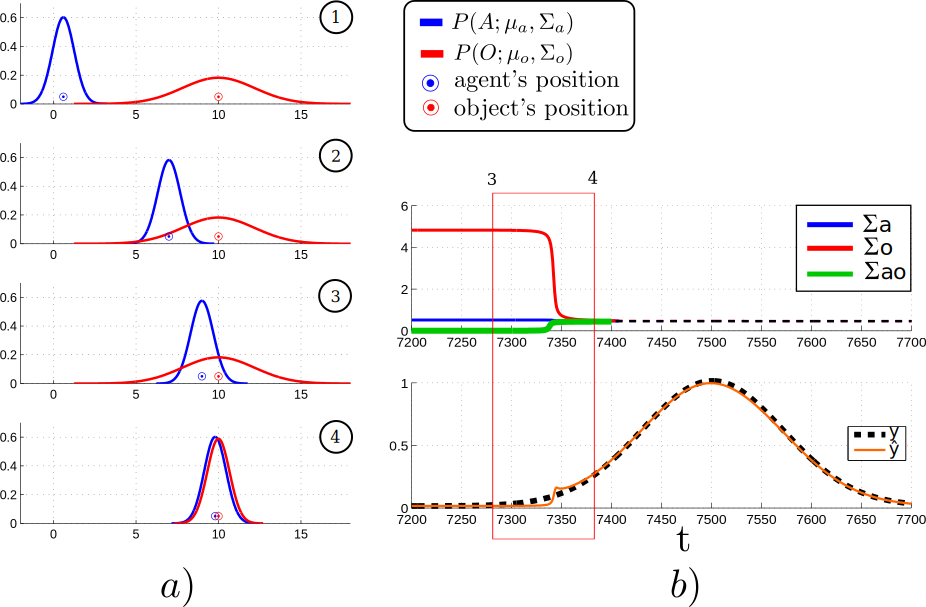
\includegraphics[width=0.9\textwidth]{./ch5-MLMF/Figures/Figure34.pdf}
\caption{\textbf{a)} Time slices of the evolution of the pdfs according to EKF-SLAM. The numbers in the top right corner of each plot indicate the 
temporal ordering.
The blue pdf represents the agent's believed location and the circle with the dot in the middle is the true location of the agent. The same holds 
for the red distribution which represents the agent's belief of the location of an object.
\textbf{b)} Evolution of the covariance components of $\Sigma$ over time and true $Y_t$ and expected measurements,  $\hat{Y}_t$. 
$\Sigma_a$ and $\Sigma_o$ are the variances of the agent and object positions and $\Sigma_{ao}$ is the cross covariance 
term.}
\label{fig:EKF-SLAM}
\end{figure}

As expected we do not get the desired behaviour, which is that the beliefs start updating as soon as they are overlapping. 
Even when most of the belief mass of the agent's location pdf overlaps that of the object pdf, no belief update occurs. 
The multivariate Gaussian of parameterisation of the BN only guarantees a dependency between the agent and object random variables 
when there is a positive sighting of the landmarks.  This can been seen in Figure \ref{fig:EKF-SLAM} (b),
where the component $\Sigma_{ao}$ is 0 most of the time which implies that $A \independent O | Y$ which is undesirable. 
This confirms that the dependencies present in the structure given by the BN are dependent on the chosen parametrisation.

\subsubsection{Histogram-SLAM}\label{sec:Discrete}

In Histogram-SLAM, the joint distribution is discretized and each bin has a parameter, 
$P(A_t=i,O=j|Y_{0:t},u_{0:t}) = \boldsymbol{\theta}^{(ij)}$, which sums to one, $\sum_{ij} \boldsymbol{\theta}^{(ij)} = 1$. 
For shorthand notation we will write $P(A_t,O|Y_{0:t},u_{0:t})$ instead of $P(A_t=i,O=j|Y_{0:t},u_{0:t})$.
The probability distribution of the agent's position is given by marginalising the object random variable:
\begin{align}
 &P(A_t|Y_{0:t},u_{0:t})    = \sum\limits_{j=1}^{|O|} P(A_t,O|Y_{0:t},u_{0:t}) \label{eq:agent_marginal} \\
 &P(A_t=1|Y_{0:t},u_{0:t})  = \sum\limits_{j=1}^{|O|} \boldsymbol{\theta}^{(1j)}
\end{align}
The converse holds true for the object's marginal over its believed position. Figure \ref{fig:histogram_joint} illustrates 
the joint distribution of both the agent and object's random variable. For ease of notation we use the shorthand $P(A)$
for $P(A_t|Y_{0:t},u_{0:t})$. The 1D world in which the agent and object are located has been discretized to 10 states,
which results in a joint distribution with 100 parameters!
If we were to discretise the state space to $N$ bins, $i=1...N$, and there is a total of $M$ random variables (one agent and $M-1$ objects)
the joint distribution would have $N^{M}$ parameters. This is an exponential increase which renders Histogram-SLAM in its naive from 
intractable.

\begin{figure}
 \centering
 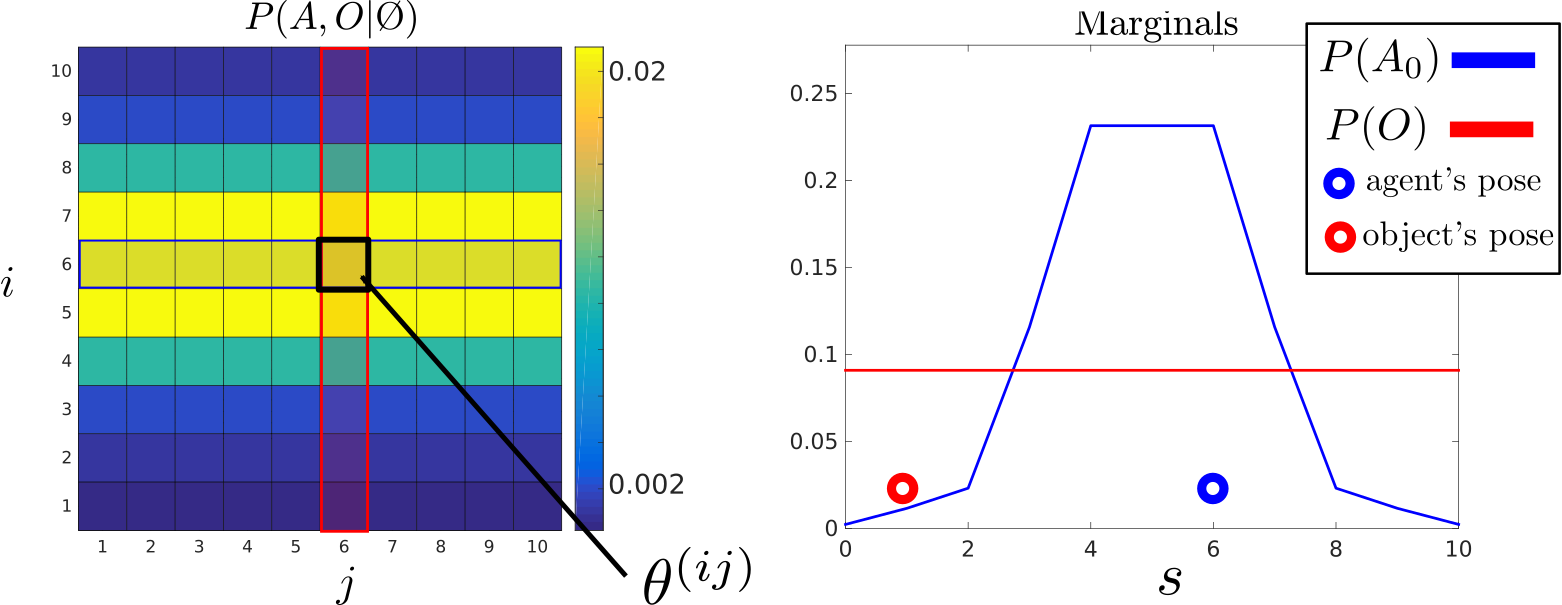
\includegraphics[width=\textwidth]{./ch5-MLMF/Figures/explenation/hist_SLAM.pdf}
 \caption{\textit{Left:} Joint distribution of the agent and object, before any action or measurement is integrated. 
 \textit{Right:} Marginals of the agent and object, it tells use the probability of their location. The marginal of each 
 random variable is obtained by marginalising the other out according to Equation \ref{eq:agent_marginal}. The probability of
 the agent and object begin in state $s=6$ is given by summing the blue and red highlighted parameters in the joint distribution. }
 \label{fig:histogram_joint}
\end{figure}

\paragraph{Histogram likelihood model}

A measurement model, $P(Y_t|A_t,O)$, predicts the likelihood of observations, $Y_t$, given the state of $A_t$ and $O$. 
In the tasks we consider, an observation occurs only if the agent enters in contact with the object, which implies that both
occupy the same discrete state. 
\begin{equation} \label{eq:ch5:discrete_likelihoood}
P(Y_t=1|A_t,O) =
  \begin{cases}
    1       & \quad \text{if } A_t = O     \\
    0  	    & \quad \text{if } A_t \not= O \\
  \end{cases}
\end{equation}

Figure \ref{fig:histogram_likelihood}, illustrates the likelihood of Equation \ref{eq:ch5:discrete_likelihoood} and for when
no contact measurement $Y_t=0$ is present in a 1D world. Both likelihoods are sparse in the sense that there is only a small 
region which gets affected by the likelihood. When there is no measurement (\textit{Left}) all the parameters of the 
joint distribution which are in the black regions will become zero, if the object is detected (\textit{Right}) then 
only parameters of the joint distribution which are within the white regions will be non-zero. All changes
to the joint distribution are constrained to the states $i = j$, which in the case of a 2-dimensional joint 
distribution is a line. This is because of the \textbf{sparsity} of the likelihood function, which will be key to 
the development of our MLMF filter.

\begin{figure}
 \centering
 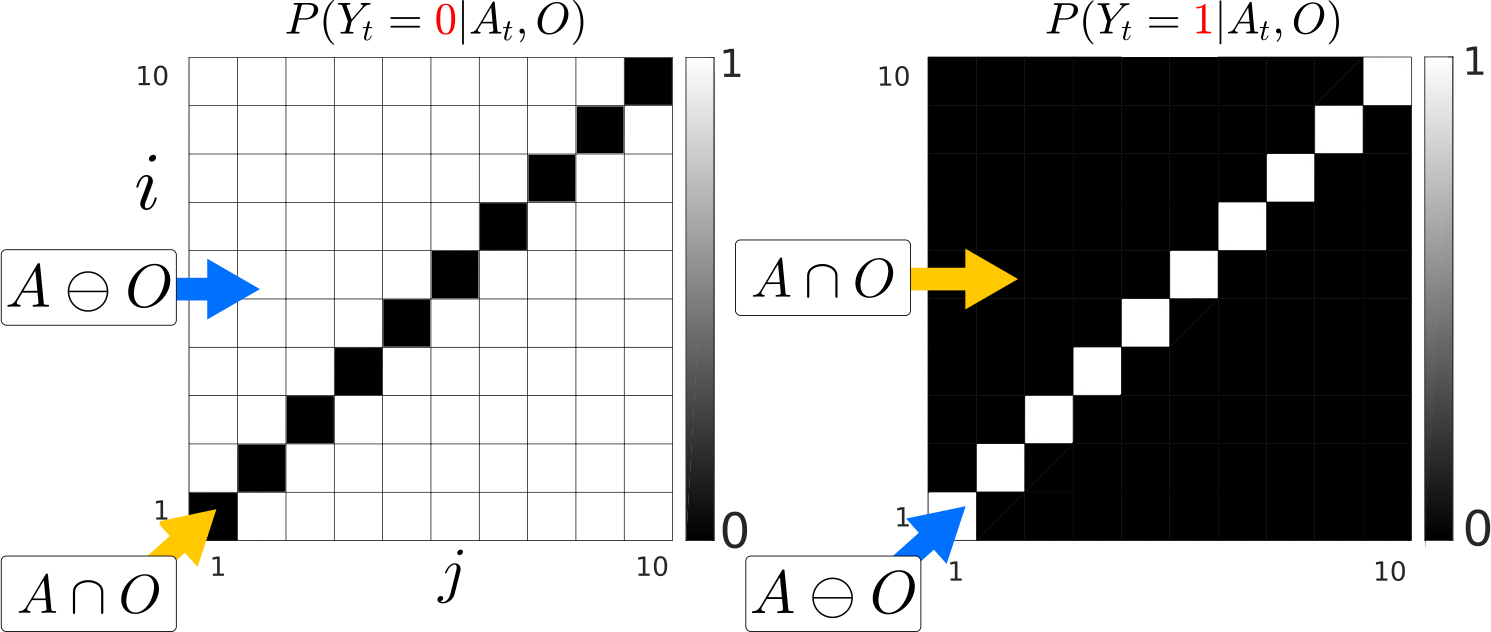
\includegraphics[width=\textwidth]{./ch5-MLMF/Figures/explenation/hist_likelihood.pdf}
 \caption{1D world Likelihood $P(Y_t|A_t,O)$. \textit{Left:} No contact detected with the object, the current measurement 
 is $\hat{Y}_t = \textcolor{red}0$, both the agent and object cannot be in the same state. \textit{Right:} The agent 
 entered into contact with the object and got a haptic feedback $\hat{Y}_t = \textcolor{red}1$. There are only two measurements 
 which the agent receives, contact or nothing.}
 \label{fig:histogram_likelihood}
\end{figure}

Two models are needed to perform the recursion, namely the motion model $P(A_t|A_{t-1},u_t)$ and the measurement model
$P(Y_t|A_t,O)$, which we already detailed. Applied one after the over to a prior joint distribution results in a posterior
distribution, both Equation \ref{eq:time-update}-\ref{eq:measurement-update} are part of the histogram Bayesian filter 
update:

\paragraph{Motion-update:}
\begin{equation}\label{eq:time-update}
   P(A_t,O|Y_{0:t-1},u_{0:t}) = \sum_{A_{t-1}} P(A_t|A_{t-1},u_t) \cdot  P(A_{t-1},O_t|Y_{0:t-1},u_{0:t-1})
\end{equation}
\paragraph{Measurement-update:}
\begin{equation}\label{eq:measurement-update}
   P(A_t,O|Y_{0:t},u_{0:t}) = \frac{P(Y_t|A_t,O)\cdot P(A_t,O|Y_{0:t-1},u_{t}) }{P(Y_t|Y_{0:t-1})}
\end{equation}

For the derivation of these  two steps, the reader is referred to Appendix \ref{appendix:bayes_recursion}.
In Figure \ref{fig:discrete_example}, we illustrate how the joint distribution evolves in a 1D world. 
The agent and object's true positions (unobservable) are in state 6 and 1. The agent moves four steps towards state 10. At each time 
step the agent does not sense the object and as a result the likelihood function  $P(Y_t=0|A_t,O)$ (Figure \ref{fig:histogram_likelihood} \textit{Left})
gets applied. As the agent moves towards the right, the motion model shifts the joint distribution towards state 10 along the agents 
dimension, $i$ (note that state 1 and 10 and wrapped).

\begin{figure}
 \centering
  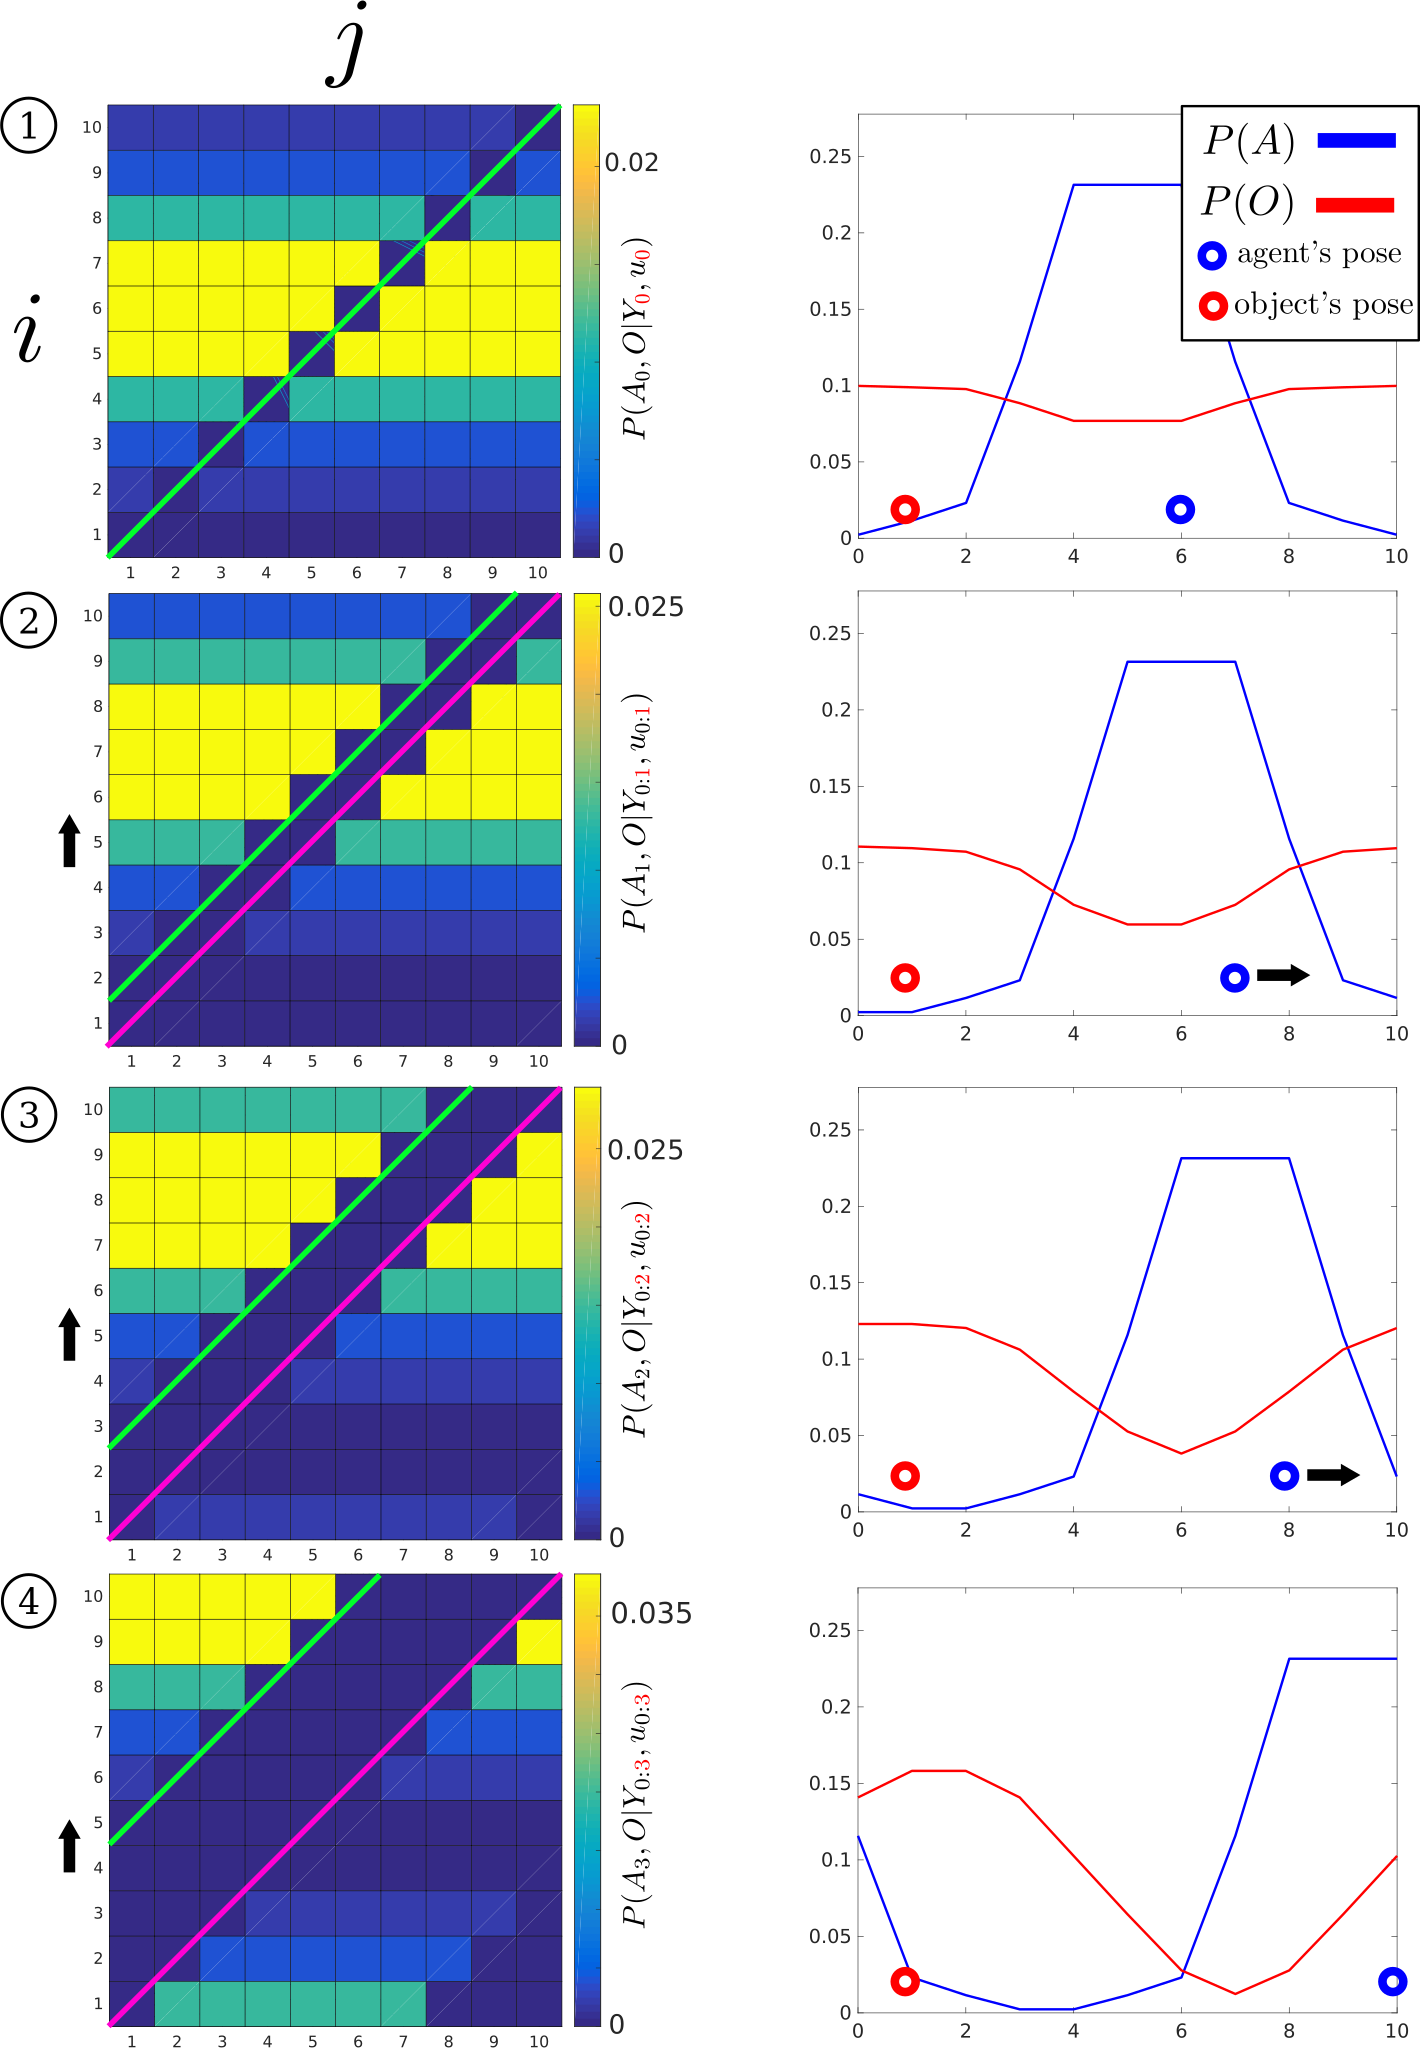
\includegraphics[width=\textwidth]{./ch5-MLMF/Figures/explenation/hist_motion.pdf}
  \caption{Histogram-SLAM, 4 time steps. \textbf{1} Application of likelihood $P(Y_0=0|A_0,O)$ and the agent remains stationary, $u_0=0$, all states along the green line become zero.
  \textbf{2} The agent moves to the right $u_1=1$, the motion $P(A_1|A_0,u_1)$, and likelihood models are applied consecutively. The right motion results in a shift (black arrow on the left) in the joint probability 
  distribution towards the state $i=10$, all parameters on the pink line are zero. \textbf{3} Same as two. \textbf{4} The original result of the likelihood function,
  green line, has moved by the same amount as the agent's displacement. At each time step a new likelihood function (pink line) is applied to the joint distribution.}
  \label{fig:discrete_example}
\end{figure}

As the agent moves to the right more parameters of the joint distribution become zero and because of the re-normalisation by the \textbf{evidence} ($P(Y_t|Y_{0:t-1}$, denominator of Equation \ref{eq:measurement-update}) the value of the remaining 
parameters increase. The amount by which the remaining parameters increase is equal to the sum of the probability mass which was set to zero by the likelihood function.
In other words the values of the joint distributions parameters which fall on the pink line in Figure \ref{fig:discrete_example} (green line also, but only for first time slice)
get set to zero and redistributed to the remaining non-zero parameters. This is an \textbf{important aspect} which will be present in MLMF and we will call this amount which has to be redistributed $\alpha \in \mathbb{R}$.

When the agent enters into contact with the object and senses it, the likelihood function $P(Y_t=1|A_t,O)$, Figure \ref{fig:histogram_likelihood} (\textit{Right}), is 
multiplied with the joint distribution with the result illustrated in Figure \ref{fig:discrete_example_contact}. Only parameters of the joint distribution whose indices
satisfy $i = j$ will remain unchanged, all the others will become zero. In retrospective the likelihood $P(Y_t=1|A_t,O)$ acts as a \textbf{constraint}, the agent and 
object have to be in the same state which is a line traversing the 2D joint distribution.

\begin{figure}
 \centering
 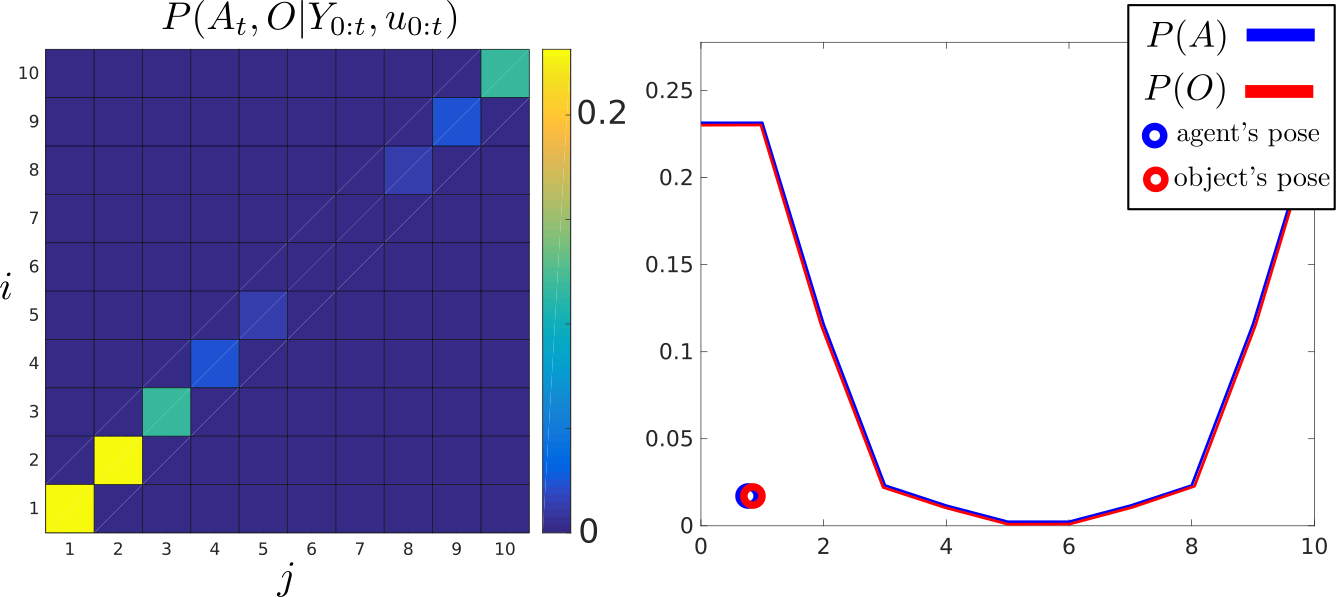
\includegraphics[width=\textwidth]{./ch5-MLMF/Figures/explenation/joint_marginal_contact.pdf}
 \caption{Histogram-SLAM contact. The agent has entered in contact with the object (measurement $Y_t = 1$) and the likelihood function $P(Y_t=1|A_t,O)$ is applied to the joint
 distribution. Only parameters on the line $i=j$ will remain unchanged and parameters for which $i \not= j$ will be set to zero.}
 \label{fig:discrete_example_contact}
\end{figure}

The \textbf{problem} with Histogram-SLAM is that its time and space complexity is exponential, as the joint distribution is discretized and 
parametrised by $\boldsymbol{\theta}^{(ij)}$. We instead propose a filter, named MLMF, which does not parameterise the joint distribution.

The main idea behind the new filter, MLMF, which we formally introduce in the next section is to achieve the same result as 
the Histogram filter but without having to parameterise the joint distribution, thus avoiding the exponential growth cost. 
The \textbf{key idea} behind the mechanism of the MLMF filter is to only evaluate the joint distribution in states $(i,j)$ for which the likelihood 
is zero and apply the updates directly to the marginals. The MLMF filter parametrises \textbf{explicitly} the marginals 
$P(A_t=s|Y_{0:t},u_{0:t}): \boldsymbol{\theta}_a^{(s)}$, $P(O=s|Y_{0:t},u_{0:t}): \boldsymbol{\theta}_o^{(s)}$. This is in contrast to the Histogram filter in which the marginals are  
derived from the joint distribution by marginalisation. For our filter to respect the Bayesian recursion, the MLMF has to \textbf{memories}
the complete history of likelihood functions $\{P(Y_t|A_t,O)\}_{t=0:T}$ and the normalization coefficient $\alpha$. The reasons 
for this will be made clear in the next section, below we summaries the parameters of the Histogram and the desired ones for the MLMF:

\begin{center}
\begin{minipage}{0.55\textwidth}
\fbox{
\begin{tabular}{lcl}
 Histogram    & : & $\boldsymbol{\theta}^{(ij)}$ \\
 desired-MLMF & : & $\boldsymbol{\theta}_a^{(s)}$, $\boldsymbol{\theta}_o^{(s)},\alpha,\{(Y,l)_p\}_{p=0:t}$\\
	      &   & $s,i,j=1,\dots,N$
\end{tabular}
}
\end{minipage}
\end{center}

The likelihood function is parametrised by a measurement, $Y_t$ and offset $l$ to the $i$-axis. In Figure \ref{fig:discrete_example} we see that
the likelihood applied at the first time step (green line) is superimposed on the line $i=j$. As actions are applied, $u_{0:3}=[1,1,1,1]$, 
the first likelihood function (green line) shifts by an amount corresponding to the total displacement (4 in this case), see the last sub-figure of
\ref{fig:discrete_example}. The second likelihood applied at $t=1$ will have an offset corresponding to the sum $u_{1:3}$, the third will have 
an offset of $u_{2:3}$ and so forth.

The MLMF, which we mathematically derive in the next section, keeps as parameters the marginals, likelihood function parameters, and a normalisation 
constant. The marginals are updated (filter recursion) by \textbf{evaluating} the joint distribution in states which are set to zero by the current 
applied likelihood and removing the value of the zeroed parameters from the marginals. 

When a positive contact is established with the object, the likelihood is zero everywhere but the states corresponding to  $i=j$, 
see Figure \ref{fig:discrete_example_contact}. In this case there is no need to evaluate the likelihood at all the zero areas 
in the joint distribution. The marginals are simply the normalisation of the line $i=j$. The evaluation of the joint distribution 
given that the object is sensed or not is restricted to the states $(i,j)$ for which $i=j$ and there is a total of $N$ of them. 
This is much less than evaluating, as it is for the histogram, $N^2$ states.


\FloatBarrier
\section{Measurement Likelihood Memory Filter}\label{ch5:MLMF}

To get the correct marginals' update, the random variables $A$ and $O$ must remain 
dependent in the absence of a positive observation $Y$ and in addition this dependence should be efficiently encoded in contrast to the
histogram parametrisation shown in Section \ref{sec:Discrete}. 

The likelihood function $P(Y_t|A_t,O)$ is the cause of the dependence between the random variables. If both the agent and object 
where completely independent, no additional parameters would be required to represent the joint distribution other than the marginals 
$P(A_t)$ and $P(O)$ giving a total of $N \cdot M$ parameters ($N$ is the number of states and $M$ is the number of random variables). 
At the other extreme if every single point in the domain of the random variables was dependent this would require the totality 
of $N^M$ parameters as previously stated in the case of the histogram filter. We propose a method in which we do not model the joint
distribution explicitly but rather only compute its impact on the marginals. 

\subsection{MLMF parametrisation}

Figure \ref{fig:margina_joint_example} shows two time slices of the evolution of the agent and object belief in a 1D world. In the \textit{left}
figure a line passes through the probability mass of the joint distribution which was initialised to be independent,
$P(A_0,O) = P(A_0) \cdot P(O)$. This is the effect the likelihood function $P(Y_t=0|A_t,O)$ has on the joint distribution given no object was sensed. As the agent 
moves towards state 100 the likelihood function is re-applied at every iteration and the result is visible in the \textit{right} figure. 
As a result the probability mass is removed from the area in the joint distribution where $P(Y_t=0|A_t,O)$ has an influence.
Because of the structure of the likelihood function, this will always in joint distribution states for which $i=j$ . 
The same is true for a range and bearing likelihood function where the range translates to the width of the tube created in the 
joint distribution. Our method will rely on remembering the applied likelihood function on the joint distribution rather than the result. 
It is far more efficient to remember a function than the values it changed in the
joint distribution.

\begin{figure}
 \centering
 \includegraphics[width=\textwidth]{./ch5-MLMF/Figures/Figure6.pdf}
 \caption{Time evolution of both the joint and marginal distributions of the agent (blue) and object (red) probability distributions for 
 the case of a 1D search. The space is discretised to 100 bins and the agent is moving in the direction of the black arrow. 
 The black line correspond to areas in which the likelihood function evaluates to zero.  \textit{Left}: the first applied 
 likelihood function, orange $t=0$, causes all the mass of joint distribution whose's states are $i=j$ to be removed. 
 The reason for this is that the agent has not sensed the object (the red and blue circles on the marginals indicate the true position of
 both the agent and the object), and all the probability mass which lies in the area of influence of the measurement likelihood gets 
 removed and redistributed to the other states in the joint distribution due to normalisation.}
 \label{fig:margina_joint_example}
\end{figure}

The parametrisation of the MLMF is derived from the Bayesian Network (BN) graphical model, Figure \ref{fig:bayesian_sse_dag}, from 
which can be derived the Bayes filter recursion  Equation \ref{eq:ch5:motion_update}, (see Appendix \ref{appendix:bayes_joint} for complete derivation). 
%However
%we do not take a recursive approach but rather remember all measurement functions which have been applied since 
%the start. %We start from the definition of the joint distribution Equation \ref{eq:bn_joint_memory} given by BN, which is the starting point to all BSSE.
%\begin{align}
% P(A_{0:t},O,Y_{0:t},u_{0:t}) &= P(A_0)P(O)\prod_{t=0}^{t} \overbrace{P(A_t|A_{t-1},u_{t})}^{=1}  \underbrace{ P(Y_t|A_t,O) }_{\mathrm{memory}} \label{eq:bn_joint_memory} %\nonumber \\
%			      &= P(A_0)P(O) \underbrace{\prod_{t=0}^{t-1} P(Y_t|A_t,O)}_{\mathrm{memory}} \label{eq:bn_joint_memory}
%\end{align}
%From Equation \ref{eq:bn_joint_memory}, we can derive the formulation of the filtering update, Equation \ref{eq:ch5:motion_update}-\ref{eq:joint_filter_memory}
%(see Appendix \ref{appendix:bayes_joint} for complete derivation).

%\begin{equation}
% P(A_0,O,Y_0) =  P(Y_0|A_0,O) P(A_0) P(O) 
%\end{equation}


\begin{center}
\begin{tikzpicture}    
\node [white_box] (box){%
\begin{minipage}{\textwidth}
\vspace*{-1cm}
\begin{align}
 &\mathrm{\textbf{intialisation}}\nonumber\\
 &P(A_0,O) = P(A_0) P(O) \\
 &\mathrm{\textbf{motion}}\nonumber\\
 &P(A_t,O,Y_{0:t-1}|u_{1:t}) = \sum_{A_{t-1}} P(A_t|A_{t-1},u_t) P(A_{t-1},O,Y_{0:t-1}|u_{1:t-1})\\ \label{eq:ch5:motion_update}
 &\mathrm{\textbf{measurement}}\nonumber\\
 &P(A_t,O,Y_{0:t}|u_{1:t}) = P(Y_t|A_{t},O) P(A_t,O,Y_{0:t-1}|u_{1:t-1}) \\
 &\mathrm{\textbf{filter (joint)}}\nonumber\\
 &P(A_t,O,Y_{0:t}|u_{1:t}) = P(O) P(A_t|u_{1:t}) \prod_{i=1}^{t}P(Y_i|A_t,O) \\
 &\mathrm{\textbf{filter (conditional)}}\nonumber\\
 &P(A_t,O|Y_{0:t},u_{0:t}) = \frac{P(A_t,O,Y_{0:t}|u_{0:t}) }{P(Y_{0:t}|u_{0:t}) } \label{eq:joint_filter_memory}
\end{align}
\end{minipage}

};
\end{tikzpicture}%
\end{center}


%\textbf{motion}\\
%\begin{minipage}{0.98\textwidth}
%\begin{equation}
% P(A_t,O,Y_{0:t-1}|u_{1:t}) = \sum_{A_{t-1}} P(A_t|A_{t-1},u_t) P(A_{t-1},O,Y_{0:t-1}|u_{1:t-1})%  \label{eq:ch5:motion_update}
%\end{equation}
%\end{minipage}
%\textbf{measurement}\\
%\begin{minipage}{0.85\textwidth}
%\begin{equation}
% P(A_t,O,Y_{0:t}|u_{1:t}) = P(Y_t|A_{t},O) P(A_t,O,Y_{0:t-1}|u_{1:t-1})
%\end{equation}
%\end{minipage}
%\begin{equation}
%  P(A_t,O|Y_{0:t},u_{0:t}) = \frac{P(Y_t|A_t,O) P(A_t,O|Y_{0:t-1},u_{0:t}) }{P(Y_t|Y_{0:t-1},u_{0:t}) } \label{eq:joint_filter_memory}
%\end{equation}

We have not unrolled the joint distribution also known as the Bayesian filter recursion, Equation \ref{eq:joint_filter_memory}, to it's recursive form  (see Appendix \ref{appendix:bayes_recursion} for the detailed derivation
of the Bayesian recursion). MLMF keeps all the \textbf{likelihood parameters} of the Bayesian filter
instead of the values $\boldsymbol{\theta}^{(ij)}$ of the joint distribution, as it is the case for Histogram-SLAM.
%P(A_{t-1},O|Y_{0:t-1},u_{0:t-1}) = &P(A_0) \cdot P(O)  \cdot  P(Y_0|A_0,O) \cdot  \nonumber \\ 
%				  &\prod\limits_{t=1}^{t-1} P(A_t|A_{t-1},u_t) \cdot P(Y_t|A_t,O)   \\
%\begin{align} 
% P(A_t,O|Y_{0:t},u_{0:t})         &= \frac{P(Y_t|A_t,O) \cdot  P(A_t,O|Y_{0:t-1},u_{0:t})  }{  P(Y_t|Y_{0:t-1}) } 
%\end{align}

The filter is composed of the original marginal distributions $P(A_0)$ and $P(O)$ and the memory of likelihood functions, Equation \ref{eq:bn_joint_memory},
which consists of the set of all likelihood functions since $t=0$ until $t$: 

\begin{equation}
 P(Y_{0:t}|A_{0:t},O;\Psi_t) := \prod_{t=0}^t P(Y_t|A_t,O) \label{eq:memory}
\end{equation}

The likelihood functions have two different functional forms (see Figure \ref{fig:histogram_likelihood}) which is dictated 
by the current measurement, which is binary and the offset of the likelihood function along the $i$-axis as we saw in
Figure \ref{fig:discrete_example} and \ref{fig:margina_joint_example}. As such the parameters of Equation \ref{eq:memory}
are all measurements since the start of the filtering and offsets along the $i$-axis, we refer to these parameters
as $\Psi_t = \{(Y,l)_p\}_{p=0:t}$. In Algorithm \ref{alg:memory-motion}, we detail how a measurement and action at 
time step $t$, result in the update of the memory; this is an algorithmic implementation of Equation  \ref{eq:ch5:motion_update},
$P(A_0)$ is considered separately.

\begin{center}
\begin{minipage}{.55\linewidth}

\begin{algorithm}[H]
\label{alg:memory-motion}
\SetKwInOut{Input}{input}
\SetKwInOut{Output}{output}

\Input{$\Psi_{t-1}$, $Y_t$, $u_t$}
\Output{$\Psi_t$}
\BlankLine
\textbf{motion update}\label{alg:ch5:motion_memory}\\
\For{$l \in \Psi_{t-1}$}{$l = l + u_t$}
\textbf{measurement update}\\
$\Psi_t \gets \{\Psi_{t-1}, (Y_t,l=0)\}$ 

\caption{memory update}

\end{algorithm} 
\end{minipage}
\end{center}

%which have been applied 
%since initialisation up to the current time step. At every time step the likelihood function get updated by the current action Equation, \ref{eq:ch5:motion_update}.
%The motion update consists of applying the forward dynamics $P(A_t|A_{t-1},u_t)$ to 
%$P(A_{t-1},O|Y_{0:t-1},u_{0:t-1})$ (Equation \ref{eq:bn_joint_memory}) to achieve $P(A_t,O|Y_{0:t-1},u_{0:t})$, see Equation \ref{eq:time_update_memory}. 
%\begin{align}\label{eq:time_update_memory}
% P(A_t,O|Y_{0:t-1},u_{0:t}) &= \sum\limits_{A_{t-1}} P(A_t|A_{t-1},u_t) \cdot  P(A_{t-1},O|Y_{0:t-1},u_{0:t-1})
%\end{align}

At every time step, the parameters of a new likelihood function, $P(Y_t|A_t,O)$, are added to Equation \ref{eq:memory}.
The motion update acts on the offset parameters $l$ of the memory function which results in the likelihood functions being shifted
along the $i$-axis as shown in Figures \ref{fig:discrete_example} and \ref{fig:margina_joint_example} and on the agent's original marginal $P(A_0)$.

The intuition of these two updates is as follows. At the first time step (after initialisation) we add the first measurement 
likelihood function which results in the line shown in Figure \ref{fig:margina_joint_example} \textit{left}; $\Psi_0 = \{(Y_0=0,u_0=0)\}$. 
Then a motion update (agent moves towards state 100) is applied and this line (or measurement
likelihood function) shifts along the agent's $i$-axis by the displacement caused by the forward motion and a new line is added at $i=j$, 
which is the result of the current measurement after the motion update. Repeating this process results in the white band present 
in Figure \ref{fig:margina_joint_example} \textit{right}. 

For ease of notation from this point onwards we will not show the conditioned actions $u_{0:t}$, so $P(A_t,O|Y_{0:t},u_{0:t})$ will 
be $P(A_t,O|Y_{0:t})$.

Our goal is to be able to compute the marginals $P(A_t|Y_{0:t})$, $P(O|Y_{0:t})$ of the agent and object random variables and 
marginal likelihood $P(Y_{0:t},u_{0:t})$ without having to perform an expensive marginalisation over the entire space of the joint distribution as it was the case for Histogram-SLAM.
We next detail how these marginals can be computed whilst avoiding computational expense.

\subsection{Computation of evidence and marginals}

In order to compute the marginal likelihood (also known as evidence) $P(Y_{0:t},u_{0:t})$ and the filtered  marginals $P(A_t|Y_{0:t})$,
$P(O|Y_{0:t})$ efficiently we take advantage of the fact that only a very small area 
in the joint distribution space will be affected by the measurement likelihood function at each time step.

Without lost of generality the likelihood function will only make a difference to dependent $A \cap O$ regions in the joint distribution, areas 
where the likelihood function evaluates smaller than one and the region inside $A \ominus O$ will not be affected, where the likelihood function 
is equal to one.
Figure \ref{fig:overlap_dependence_independence} shows the relation between the measurement 
function $P(Y_t|A_t,O)$ and the joint distribution $P(A_t,O|Y_{0:t})$ for three different initialisations. 

%effect on the joint distribution for three different initialisations. 
%
%  The tube's boundary is governed by the bandwidth of the radial basis function of the likelihood function.
%  Any probability mass of the joint  distribution which lies in the tube will be in the $\cap$, all probability 
%  mass outside the tube but still within the grey rectangle is located in $\ominus$ and 
%  the white space is in the domain but not parametrised and thus not considered.
 
 \begin{figure}
 \centering
  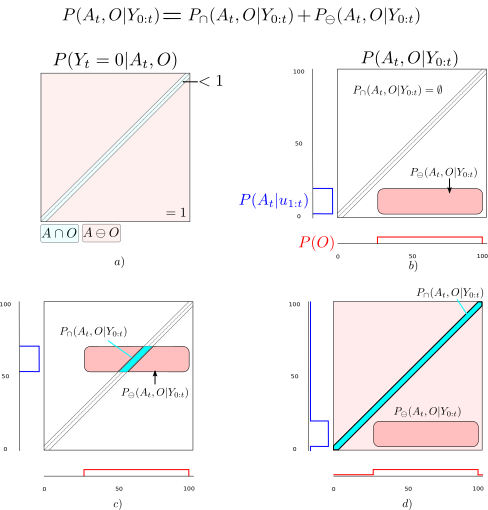
\includegraphics[width=\textwidth]{./ch5-MLMF/Figures/Figure7.pdf}
  \caption{
  \textbf{a)} Likelihood $P(Y_t=0|A_t,O)$, the blue area depicts the regions in which the likelihood is $<1$ 
  and the red area is where the likelihood is $=1$. If the probability mass of the joint distribution 
  is in the blue region, then the parameters of the random variables in these areas are dependent, $A \cap O$
  and if not then they are independent from one another, $A \ominus O$.  
   \textbf{b)} The agent and object marginals are not overlapping and thus are completely independent. The joint distribution 
   ,$P(A_t,O|Y_{0:t})$ the black rectangle,  is not intersecting with the measurement function. As a result $P_{\cap}(A_t,O|Y_{0:t})$
   is empty.
 \textbf{c)} The marginals overlap one another resulting in the measurement likelihood function intersection with the joint distribution.
 The joint distribution is composed of the blue and red areas, Equation \ref{eq:joint_independent_dependent}.
 The probability mass at the intersection gets removed and renormalised to other regions which is the result of applying Bayes integration. 
 \textbf{d)} The marginals of $A$ and $B$ are completely overlapping, however only a small fraction of the probability mass 
 in the joint distribution is within the measurement function's tube.}
  \label{fig:overlap_dependence_independence}
\end{figure}
%\end{FPfigure}

As illustrated and explained in Figure \ref{fig:overlap_dependence_independence}, the joint distribution can be decomposed in a 
dependent and independent term (Equation \ref{eq:joint_independent_dependent}). 

\begin{equation}\label{eq:joint_independent_dependent}
 P(A_t,O|Y_{0:t}) = P_{\cap}(A_t,O|Y_{0:t}) + P_{\ominus}(A_t,O|Y_{0:t})
\end{equation}

The probability mass covered by the dependent term is located within the measurement function's tube and the independent probability mass 
is located outside as shown in Figure \ref{fig:overlap_dependence_independence}. This formulation will lead to large computational gain 
as the independent term is not influenced by the measurement function: 
$P_{\ominus}(A_t,O|\mathbf{Y_{0:t}}) \propto P_{\ominus}(A_t,O|\mathbf{Y_{0:t-1}})$.

\paragraph{Evidence}\\
The evidence of the measurement $P(Y_{0:t},u_{0:t})$ is the amount of probability mass which has been removed from the region of the joint 
distribution where the likelihood function has evaluated the parameters of the joint distribution to zero. At time step $t$, the normalising factor to be added to 
the evidence is the difference between the probability mass located inside $A\cap O$ before the application of the measurement 
function $P(Y_t|A_t,O)$ and after, see Equation \ref{eq:I} (see Appendix \ref{appendix:evidence} for the full derivation).

\begin{align}\label{eq:I}
 &\alpha_t 	  = \sum\limits_{A_t}\sum\limits_{O} P_{\cap}(A_t,O|Y_{0:t-1}) (1 - P(Y_t|A_t,O)) \\
 &P(Y_{0:t},u_{0:t})      = 1 - (\alpha_{0} + \alpha_{1} + \cdots + \alpha_{t})
\end{align}
The advantage of Equation \ref{eq:I} is that the summation is only over states which are in the dependent area $\cap$ of the joint 
distribution. This is generally always much smaller than the full space itself.
Until an object is sensed, the likelihood will always be zero $P(Y_t|A_t,O) = 0$ and $\alpha$ will correspond to the probability 
mass which falls within the region of the joint distribution in which the likelihood function is zero. In Figure 
\ref{fig:overlap_dependence_independence} (\textit{Middle \& Right}) the sum of the probability mass in the blue 
regions is equal to $\alpha$.
The point of interest is that as we perform the filtering process we will never renormalise the whole joint distribution, but only keep 
track of how much it should have been normalised. To this end the original marginals $P(A_0)$ and $P(O)$  are never renormalised but are used 
to compute at each step how much of the probability mass $\alpha_t$ should go to the normalisation factor $P(Y_{0:t},u_{0:t})$. 
The evidence in question will never be negative, as the joint distribution sums to one and each $\alpha_t$ represents some of the mass removed from the joint distribution. Since we 
keep track of the history of applied  measurement likelihood functions we never remove the same amount of probability mass twice
from the joint distribution.

\paragraph{Marginals}

%The computation of the marginal is similar to that of the evidence. The difference is that we do not marginalise the 
%random variable being queried, so there is one less summation.
The marginal of the agent and object random variable is acquired through marginalisation:
\begin{align}
  &P(A_t|Y_{0:t}) = \sum\limits_{O}   P(A_t,O|Y_{0:t}) = \overbrace{\sum\limits_{O} P_{\cap}(A_t,O|Y_{0:t})}^{P_{\cap}(A_t|Y_{0:t})} + \overbrace{\sum\limits_{O} P_{\ominus}(A_t,O|Y_{0:t})}^{P_{\ominus}(A_t|Y_{0:t})}   \nonumber \\
  &P(O|Y_{0:t})   = \sum\limits_{A_t} P(A_t,O|Y_{0:t}) = \sum\limits_{A_t} P_{\cap}(A_t,O|Y_{0:t}) + \sum\limits_{A_t} P_{\ominus}(A_t,O|Y_{0:t})\nonumber
\end{align}
In Histogram-SLAM, to get both the agent and object marginals, at every time step, the joint distribution is marginalised.
This requires storing and summing over all the parameters of the joint distribution which is expensive. Instead in MLMF 
we will take advantage of the sparsity of the likelihood function and as a result we can decompose the marginal into both 
dependent $\cap$ and independent $\ominus$ components. In MLMF, in contrast to Histogram-SLAM, we only parameterise
the marginals (not the full joint distribution) and update them where measurements have an effect,  Equation \ref{eq:marignal_mrf}
(see Appendix \ref{appendix:marginal} for the full derivation of Equation \ref{eq:marignal_mrf}).

%As for the evidence, the marginal is evaluated only in areas of the joint distribution which are dependent and uses the previously 
%computed evidence to normalise this region of the joint distribution during the marginalisation process, Equation \ref{eq:marignal_mrf}
\begin{equation}
 P(A_t|Y_{0:t})  =  P(A_t|Y_{0:t-1}) - \Big(P_{\cap}(A_t|Y_{0:t-1}) -  \mathbf{P_{\cap}(A_t|Y_{0:t}})  \Big) \label{eq:marignal_mrf} 
\end{equation}
\begin{align}\label{eq:marignal_mrf_2}
 \mathbf{P_{\cap}(A_t|Y_{0:t})} &= \frac{ \sum\limits_{O} \overbrace{ P(Y_t|A_{t},O)  \sum_{A_{t-1}} P(A_t|A_{t-1},u_t)  P(A_{t-1},O,Y_{0:t-1},u_{0:t-1})  }^{P_{\cap}(A_t,O,Y_{0:t},u_{0:t})}}{\underbrace{1  - (\alpha_{0} + \alpha_{1} + \cdots + \alpha_{t})}_{P(Y_{0:t},u_{0:t})}} \\
		       &= \sum\limits_{O} P_{\cap}(A_t,O|Y_{0:t})
\end{align}

\begin{figure}
\centering
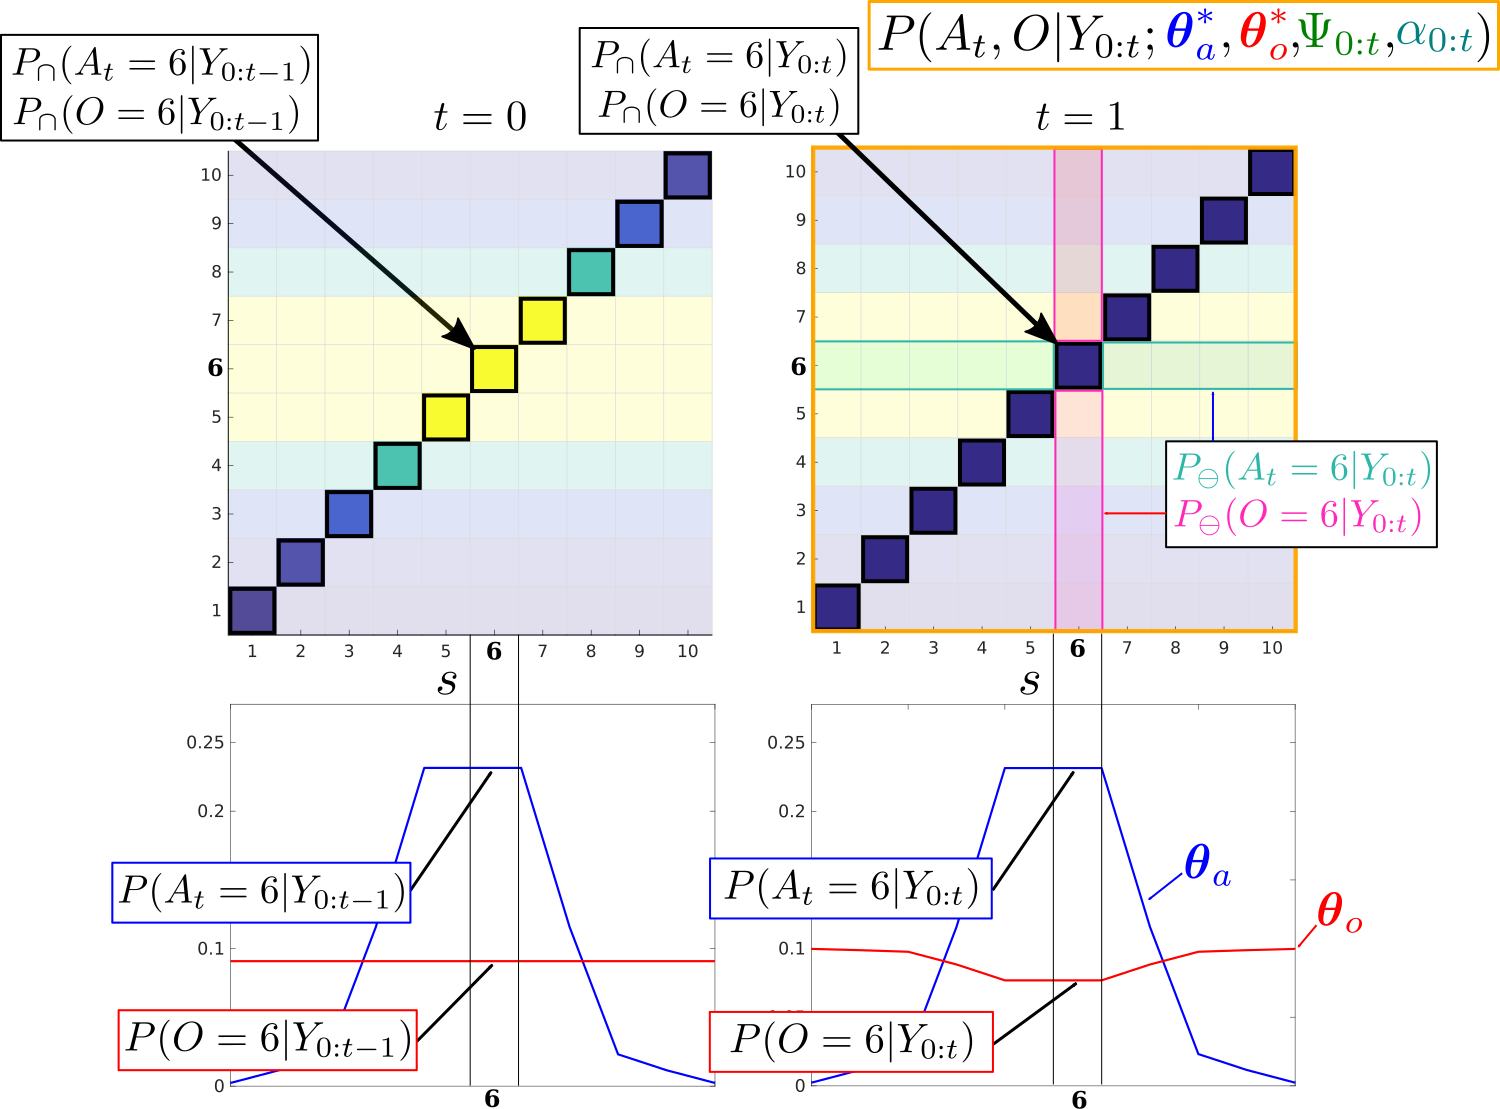
\includegraphics[width=0.95\textwidth]{./ch5-MLMF/Figures/explenation/marginal_cal_example.pdf}
\caption{Marginal update, illustration of the agent and object marginal update, Equation \ref{eq:marignal_mrf}. The parameters of the joint 
distribution are dimmed, with the exception of dependent areas, where $P(Y_t<1|A_t,O)$, which corresponds to the diagonal $i=j$. The MLMF only
evaluates the joint distribution where the likelihood changes the joint's parameters. For each state of the marginals $1,\cdots,10$ the difference 
of the marginals inside the dependent area, before and after the measurement likelihood is applied, is evaluated and removed from the marginals 
$P(A_t|Y_{0:t-1})$, $P(O|Y_{0:t-1})$ leading to $P(A_t|Y_{0:t})$, $P(O|Y_{0:t})$. }
\label{fig:ch5:marginal_update}
\end{figure}

Equation \ref{eq:marignal_mrf} is a recursive, $P(A_t,|Y_{0:\mathbf{t}})$ is computed in terms of  $P(A_t,|Y_{0:\mathbf{t-1}})$.
In Figure \ref{fig:ch5:marginal_update} we illustrate how the MLMF updates the marginals of the agent and object given a new measurement.


In table \ref{tab:mlmf_parameters} we summaries the functions and parameters of the MLMF for two random variables, an agent and object.
\begin{table}[h]
\centering
\fbox{
\begin{tabular}{lcll}
    functions             &   & parameters                      & description \\\hline
  $P(A_t|Y_{0:t})$        & : & $\boldsymbol{\theta}_a$	      & filtered marginals\\
  $P(O|Y_{0:t})$          & : & $\boldsymbol{\theta}_o$	      &  \\
  $P(A_0)$     	          & : & $\boldsymbol{\theta}^*_a$       & initial beliefs\\
  $P(O)$                  & : & $\boldsymbol{\theta}^*_o$       & \\
  $P(Y_t|Y_{0:t-1})$      & : & $\alpha \in \mathbb{R}$         & evidence\\
  $P(Y_{0:t}|A_{0:t},O)$  & : & $ \Psi = \{(Y,l)_p\}_{p=0:t}$ & likelihood history
\end{tabular}
}
\caption{MLMF functions with associated parameters. The marginal parameters are the discretisation of the 
state space $\boldsymbol{\theta} \in \mathbb{R}^N$, $\boldsymbol{\theta}^{(k)}$ corresponds to the probability being in state $k$.}
\label{tab:mlmf_parameters}
\end{table}

\subsection{MLMF-SLAM Algorithm}

\begin{center}
\begin{minipage}{\linewidth}

\begin{algorithm}[H]
\label{alg:mrf-slam}
\SetKwInOut{Input}{input}
\SetKwInOut{Output}{output}
\Input{$P(A_{t-1})$, $P(O)$, $P(A_{t-1}|Y_{0:t-1},O)$, $P(O|Y_{0:t-1})$ \\ $P(Y_{0:t-1}|A_{0:t-1},O)$ \\ $Y_t$, $u_t$}
\Output{$P(A_t)$, $P(A_t|Y_{0:t})$, $P(O|Y_{0:t})$, $P(Y_{0:t}|A_{0:t},O)$}
\BlankLine
\textbf{motion update}\\
$P(A_t|Y_{0:t-1})  = \sum\limits_{A_{t-1}} P(A_t|A_{t-1}) \cdot P(A_{t-1}|Y_{0:t-1})$\\
$P(A_t)  = \sum\limits_{A_{t-1}} P(A_t|A_{t-1},u_t) \cdot P(A_{t-1})$\\
$P(Y_{0:t-1}|A_{0:t},O) \gets$ motion update Algorithm \ref{alg:ch5:motion_memory} 
\BlankLine
\textbf{measurement update}
\BlankLine
$P(A_t|Y_{0:t}) = P(A_t|Y_{0:t-1}) - \Big(P_{\cap}(A_t|Y_{0:t-1}) -  P_{\cap}(A_t|Y_{0:t}) \Big)$  \\
$P(O|Y_{0:t}) = P(O|Y_{0:t-1}) -  \Big(  P_{\cap}(O_t|Y_{0:t-1}) -  P_{\cap}(O_t|Y_{0:t})\Big)$    \\
$\alpha = \alpha +  \sum\limits_{A_t}\sum\limits_{O} P_{\cap}(A_t,O|Y_{0:t-1}) (1 - P(Y_t|A_t,O))$ \\
$P(Y_{0:t}|A_{0:t},O) \gets$ measurement update Algorithm \ref{alg:ch5:motion_memory} 
\caption{MLMF-SLAM}
\end{algorithm} 
\end{minipage}
\end{center}
In Algorithm \ref{alg:mrf-slam} we give the motion-measurement update recursion for the MLMF-SLAM.
This formulation is advantageous as the joint distribution is only evaluated inside the regions 
$A\cap O$ created in the joint space by the likelihood function. Through the term $P(Y_{0:t}|A_t,O)$ we keep 
track of the normalisation factor $P(Y_t|Y_{0:t-1})$ which 
is a scalar, and where we have previously applied the likelihood function. 

We evaluated this formulation of the joint distribution with the standard histogram filter in the case of the 1D search routine 
illustrated in Figure \ref{fig:margina_joint_example} and we found them to be identical. We stayed true to the formulation of Bayes rule 
and thus assert that Algorithm \ref{alg:mrf-slam} is a Bayesian Optimal Filter/Solution
\footnote{An optimal Bayesian solution is an exact solution to the recursive problem of calculating the exact posterior density 
\cite{PF_tutorial_2002}}.

\subsection{Space \& time complexity (MLMF)}\label{ch5:space_time_complexity_MLMF}

For discussion purposes we consider the case of three beliefs, namely that of the agent and two other objects $O^{(1)}$ and $O^{(2)}$ but 
subsequently we generalise. As stated previously $M$ stands for the number of filtered random variables including the agent. When we refer 
to only the objects we say that we have $M-1$ random variables. $N$ is the number of discrete states in the world. We contrast
the MLMF-SLAM with Histogram-SLAM.

%At every time step we store the action, $u_t \in D$, only if the current marginals have changed as a result of the measurement likelihood function, $P(Y_t|A_t,O)$.


\subsubsection{Space complexity}

Figure \ref{fig:3bel_lik_profile} \textit{left} illustrates the volume occupied by the joint distribution for a marginal space of $N$ states. 
Histogram-SLAM would require $N^3$ parameters for the joint distribution $P(A,O^{(1)},O^{(2)})$ and $N^{M}$ for $M$ random variables. 

For MLMF-SLAM, each random variable $X$ requires two sets parameters $\boldsymbol{\theta}$ and $\boldsymbol{\theta}^*$ 
(see Table \ref{tab:mlmf_parameters}). Given
$M$ random variables, the initial number of parameters is $M \cdot (2 \cdot N)$.
At every time step the likelihood memory function increments by one measurement and offset, $(Y_t,l=0)$ (Algorithm \ref{alg:ch5:motion_memory}).
Given a state space of size $N$, there can be no more than $N$ different measurement functions (one for each state). In
the worst case scenario the space complexity of the memory will be $N$, giving a total of $M \cdot (2 \cdot N) + N$. 
The final worst case space complexity is linear in the number of random variables, $\BigO(N\,M)$. 

\begin{figure}
 \centering
  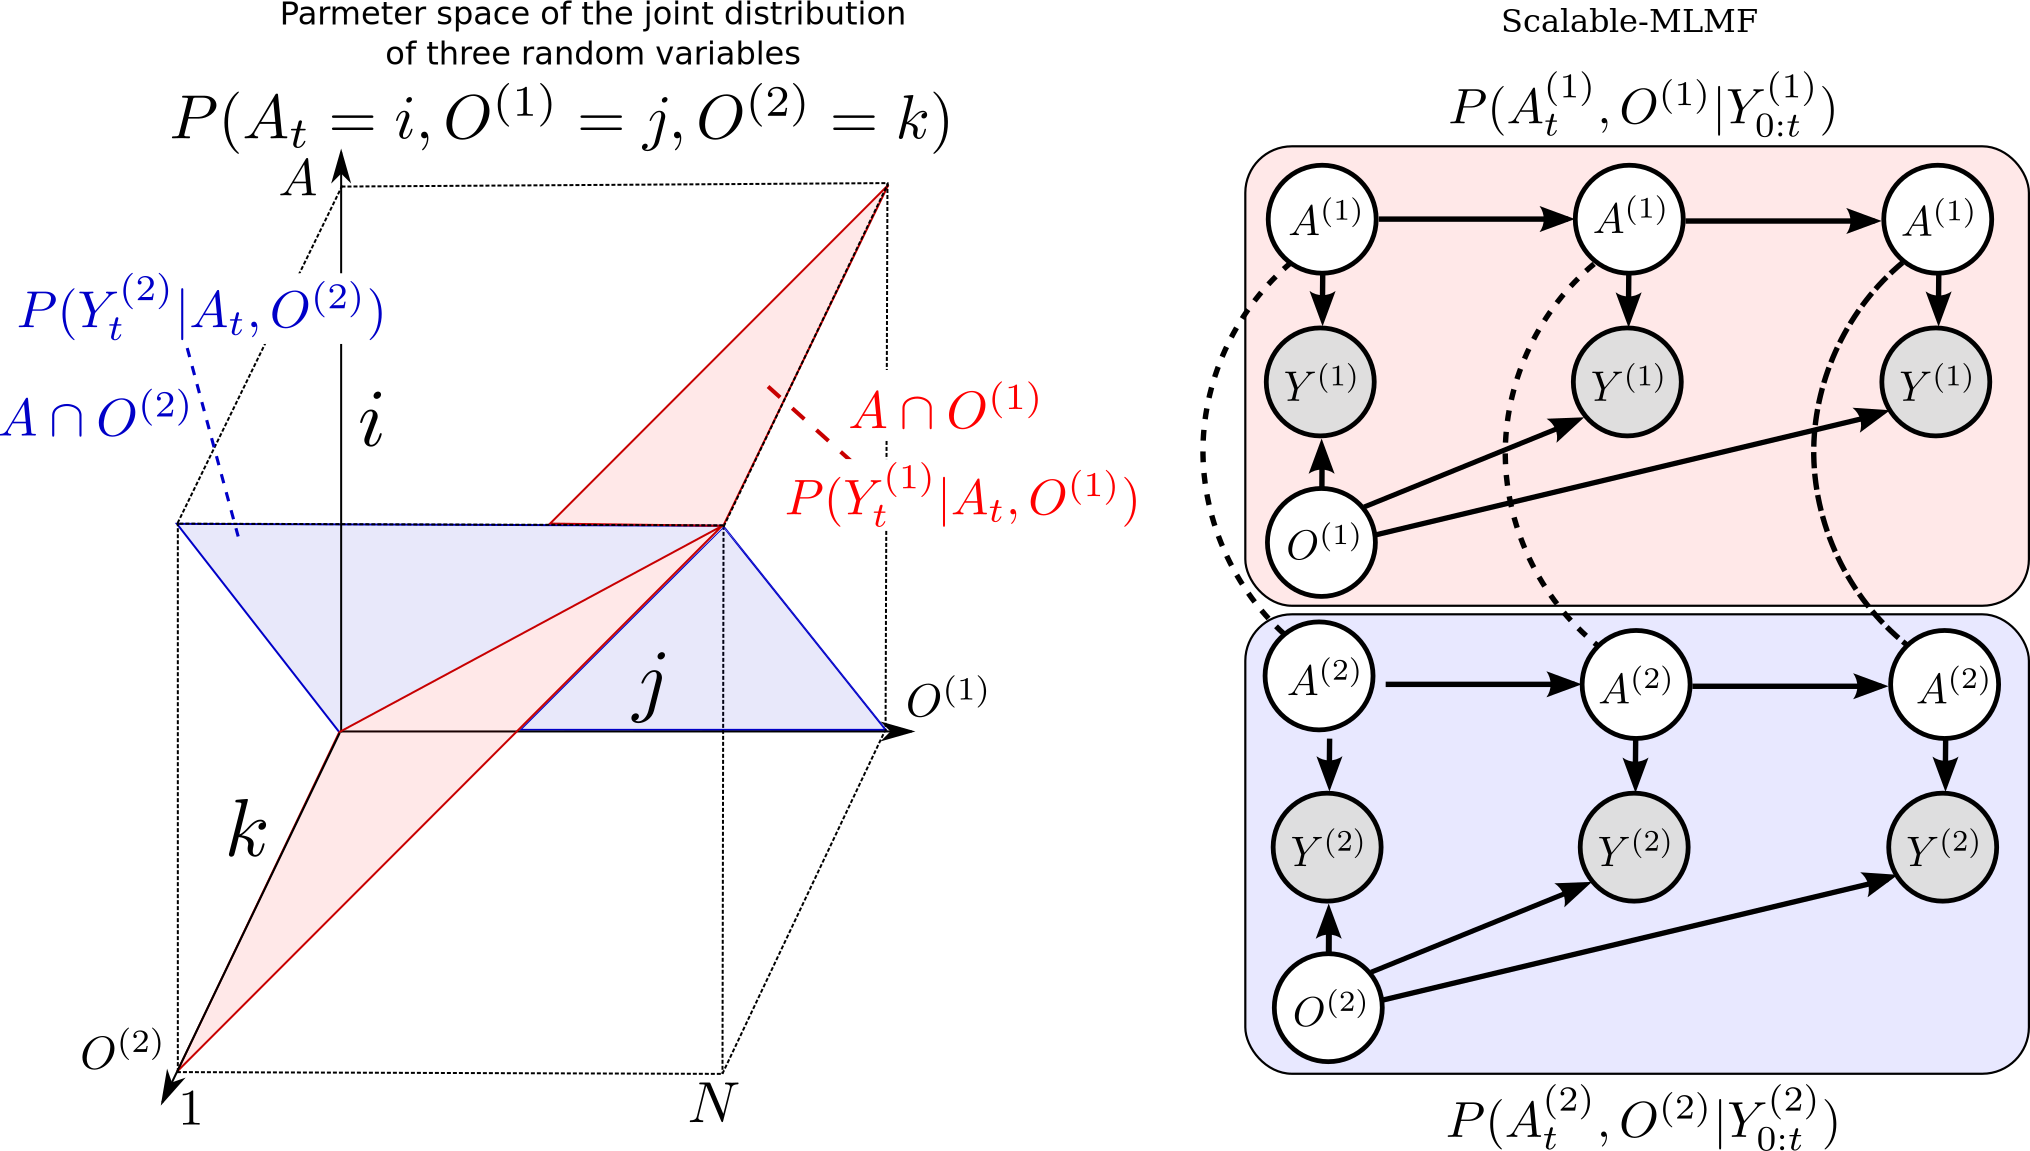
\includegraphics[width=\textwidth]{./ch5-MLMF/Figures/Figure8_v2.pdf}
  \caption{\textit{Left:} Joint distribution $P(A,O^{(1)},O^{(2)})$ of the agent and two objects. Each measurement likelihood function, $P(Y|A,O^{(1)})$, 
  $P(Y|A,O^{(2)})$ corresponds to a hyperplane in the joint distribution
  The state space is discretised to $N$ bins giving the total number of parameters in the joint distribution of $N^3$. 
  \textit{Right:} \textbf{Scalable-MLMF} Each agent-object joint distribution pair is modelled independently. For clarity we have left 
  out the action random variable $u$ which is linked to every agent node.
  Two joint distributions $P(A^{(1)},O^{(1)}|Y^{(1)}_{0:t})$   and $P(A^{(2)},O^{(2)}|Y^{(2)}_{0:t})$ parametrise the graphical model. 
  The dashed undirected lines represent a wanted dependency, if present $O^{(1)}$ and $O^{(2)}$ are to be dependent through $A$. In
  the standard setting there will be no exchange of information between the individual joints. However we demonstrate later on how
  we perform a one time transfer of information when one of the objects is sensed.}
  %\textit{Right:} Joint distribution of the agent and one object $P(A_t,O|Y_{0:t})$.
  %Three measurement 
  %functions have been added to the memory term. At every time step when an action is taken all measurement functions are updated according to 
  %the action applied $u_t$. This means that the first function to be added to the memory will have had all actions applied to it. The number 
  %of the equations and their associated lines in the plot indicate the order in which they have been added to the memory. 
  %The three points are candidates at which we want to evaluate the joint distribution.  The cost of evaluating the 
  %joint distribution at the yellow point is $\BigO(1)$ since we only have to check the first element in the memory. 
  %For the green and cyan points the cost is $\BigO(\log(n))$, where $n$ is the number of likelihood functions in memory.}
  \label{fig:3bel_lik_profile}
\end{figure}

\subsubsection{Time complexity}

For Histogram-SLAM, the computational cost is equivalent to that of the space complexity, $\BigO(N^M)$,
since to obtain all the marginals, every state in the joint distribution has to be summed.

For MLMF-SLAM, every state in the joint distribution's state space which has been changed by the measurement likelihood function 
has to be summed, see Figure \ref{fig:ch5:marginal_update}. As a result the computational complexity is directly related to the number 
of dependent states $|A \cap O|$. In Figure \ref{fig:3bel_lik_profile} \textit{left}, the number of effected states are those in the blue
and red plane (the states in the green plane will only be changed once because the agent's motion is parallel to it).
For $M$ random variables the computational cost is $\BigO(N^{M-1})$ as opposed to $\BigO(N^M)$. 
The computation complexity in this setup is still exponential but to the order $M-1$ as opposed to $M$ which will nevertheless quickly limits 
the scalability as more objects are added. 

%\paragraph{Evaluation of a state in the joint distribution}
%In Figure \ref{fig:3bel_lik_profile} (right) we show three different points in the joint distribution to be evaluated. 
%The memory of applied measurement functions is searched to see if any have effected the values at the three chosen the states. 
%The memory functions are sorted according to their offset from the axis $i=j$. For the yellow point the cost is 
%of $\BigO(1)$ since we only have to check the first (last) element in the list. For the green and blue point the 
%search is $\BigO(\log(n))$, where $n$ is the number of stored memory functions (there can be no more than $N$, the total number of states). 

\subsection{Scalable extension to multiple objects}\label{subsec:scalabe_extension}

To make our filter scalable we introduce an \textbf{independence assumption} between the objects and model the joint distribution (Equation \ref{eq:pair_wise_joint}) as the product 
of agent-object pairs:

\begin{equation}\label{eq:pair_wise_joint}
 P(A_t,O^{(1)},\cdots,O^{(M-1)}|Y_{0:t}) = \prod\limits_{i=1}^{M-1} P(A^{(i)}_t,O^{(i)}|Y^{(i)}_{0:t})
\end{equation}

The measurement variable $Y_t$, is the vector of all each agent-object 
measurement, $Y_t = \left[Y^{(1)}_t,\dots,Y^{(M-1)}_t\right]^{\mathrm{T}}$. Each agent-object joint distribution has its own parametrisation of the agent's marginal,
$A^{(1)}_t,\dots,A^{(M-1)}_t$ which combine to give the overall marginal of the agent $A_t$.

%\begin{figure}
%\centering
%  \includegraphics[width=0.5\textwidth]{./ch5-MLMF/Figures/Figure9.pdf}
%  \caption{\textbf{Scalable filter} Each agent-object joint distribution pair is modelled independently. For clarity we have left 
%  out the action random variable $u$ which is linked to every agent node.
%  Two joint distributions $P(A^{(1)},O^{(1)}|Y^{(1)}_{0:t})$   and $P(A^{(2)},O^{(2)}|Y^{(2)}_{0:t})$ parametrise the graphical model. 
%  The dashed undirected lines represent a wanted dependency, if present $O^{(1)}$ and $O^{(2)}$ are to be dependent through $A$. In
%  the standard setting there will be no exchange of information between the individual joints. However we demonstrate later on how
%  we perform a one time transfer of information when one of the objects is sensed.}
%  \label{fig:scalable_mlmf_dae}
%\end{figure}

The computation of each object marginal $P(O^{(i)}|Y^{(i)}_{0:t})$ is independent of the other objects. This is evident from the marginalisation 
see Equation \ref{eq:marg_indep}-\ref{eq:marg_indep_prod}.

\begin{align}
 P(O^{(i)}|Y^{(i)}_{0:t}) &= \sum\limits_{A^{(i)}_t} P(A^{(i)}_t,O^{(i)}|Y^{(i)}_{0:t}) \label{eq:marg_indep} \\
 P(A_t|Y_{0:t})           &= \prod\limits_{i=1}^{M-1} \left(\sum\limits_{O_i} P(A^{(i)}_t,O^{(i)}|Y^{(i)}_{0:t})\right)  \\
	                  &= \prod\limits_{i=1}^{M-1} \ P(A^{(i)}_t|Y^{(i)}_{0:t}) \label{eq:marg_indep_prod}
\end{align}

The independence assumption will create an unwanted effect with respect to agent's marginal $P(A_t|Y_{0:t})$. 
At initialisation the agent marginals should be equal, $P(A_0|Y_0) = P(A^{(i)}_0|Y^{(i)}_0) \forall_i$, however this is not the case because of 
Equation \ref{eq:marg_indep_prod}. To overcome this we define the final marginal, $P(A_t|Y_{0:t})$, of the agent as being the average of all the individual
pairs $P(A^{(i)}|Y^{(i)}_{0:t})$.

\begin{equation}
  P(A_t|Y_t) := \frac{1}{M-1} \sum\limits_{i=1}^{M-1} \ P(A^{(i)}_t|Y^{(i)}_t) \label{eq:marg_indep_sum}
\end{equation}

Figure \ref{fig:3bel_lik_profile} (\textit{Right}), depicts the graphical model of the scalable formulation. 
As each joint distribution pair has its own parametrisation of the agent's marginal and these do not subsequently get updated by one another,
the information gained by one joint distribution pair is \textbf{not transferred}.
A remedy is to transfer information between the marginals $A^{(i)}$ at specific intervals namely when one of the objects is sensed by the agent. 

\begin{center}
\begin{minipage}{\linewidth}

\begin{algorithm}[H]
\label{alg:scalabe-mrf-slam}
\SetKwComment{Comment}{$\triangleright$\ }{}
\SetKwInOut{Input}{input}
\SetKwInOut{Output}{output}
\Input{$P(A^{(i)}_t)$, $P(A^{(i)}_t|Y^{(i)}_{0:t-1})$\\$P(O^{(i)})$, $P(O^{(i)}|Y^{(i)}_{0:t-1})$\\ $Y^{(i)}_t$\\$i=1,\cdots,M$}
\BlankLine

\Comment{If object $i$ has been sensed by the agent}
\eIf{$Y^{(i)}_t > 0$}{
% \Comment*[r]{measurement update Algo. \ref{alg:mrf-slam} }
$P(O^{(i)}|Y^{(i)}_{0:t})   \gets P(O^{(i)}|Y^{(i)}_{0:t-1})$  \Comment*[r]{measurement update Algo. \ref{alg:mrf-slam}} 
$P(A^{(i)}_t|Y^{(i)}_{0:t}) \gets P(A^{(i)}_t|Y^{(i)}_{0:t-1})$\\


\ForAll{$j\in(1,\dots M-1) \setminus i$}
{
$P(A^{(j)}_t|Y_{0:t}) = P(A^{(i)}_t|Y_{0:t})$ \\
$P(A^{(j)}_t) = P(A^{(i)}_t)$\\
$P(O^{(j)}|Y^{(i)}_{0:t}) \leftarrow \sum\limits_{A^{(j)}} P(A^{(j)}_t,O^{(j)}|Y^{(i)}_{0:t})$ \Comment*[r]{object $j$ marginal} 
}

}{

\ForAll{$i\in(1,\dots M)$}{
  measurement update Algo. \ref{alg:mrf-slam}
}
}
\caption{Scalable-MLMF: Measurement Update}
\end{algorithm} 
\end{minipage}
\end{center}


The exchange of information of one joint distribution to another is achieved through the agent's marginals $A^{(i)}$ according to Algorithm \ref{alg:scalabe-mrf-slam}.
The measurement update is the same as previously described in Algorithm \ref{alg:mrf-slam} in the case of no positive measurements of the objects. If the agent
senses an object, all of the agent marginals of the remaining joint distributions are set to the marginal of the joint distribution pair belonging to the positive 
measurement $Y^{(i)}_t$. 

\begin{figure}
  \centering
  \fbox{\includegraphics[width=0.8\textwidth]{./ch5-MLMF/Figures/Figure10.pdf}}
  \caption{\textbf{Transfer of information between joint distributions} \textit{top left and right:} Joint distributions of 
   $P(A^{(1)}_t,O^{(1)}|Y^{(1)})$ and $P(A^{(2)}_t,O^{(2)}|Y^{(2)})$ prior and post sensing. The red and blue lines correspond 
  to the region in which the measurement functions $P(Y^{(1)}_{t}|A^{(1)}_t,O^{(1)})$ and $P(Y^{(2)}_{t}|A^{(2)}_t,O^{(2)})$ will change the joint distributions.
  The dotted black lines are for ease of comparing the joint distributions prior and post sensing.
  \textit{bottom right:}  After the agent has sensed $O^{(2)}$, all the probability mass which was not overlapping the blue line becomes an infeasible
  solution to the agent and object locations. \textit{bottom left:} The constraint imposed by the measurement likelihood function of the second object
  (blue line) is transferred to the joint distribution of the first object according to Algorithm \ref{alg:scalabe-mrf-slam}.
  The result is a change in the joint distribution  $P(A^{(1)}_t,O^{(1)}|Y^{(1)})$, which satisfies the constraints 
  imposed by the agent's marginal from the joint distribution $P(A^{(2)}_t,O^{(2)}|Y^{(2)})$.}
  \label{fig:transfer_information}
\end{figure}

Figure \ref{fig:transfer_information}, depicts the process of information exchange between object $O^{(1)}$ and $O^{(2)}$ in the event that the agent 
gets a positive sensation of $O^{(2)}$. Prior to the positive detection both marginals $P(A^{(1)}_t|Y^{(1)}_{0:t-1})$ and $P(A^{(2)}_t|Y^{(2)}_{0:t-1})$ 
occupy the same region and are identical. When the agent senses $O^{(2)}$ the line defined by the measurement 
likelihood function $P(Y^{(2)}_t|A^{(2)}_t,O^{(2)})$ becomes a hard constraint implying that both the agent and $O^{(2)}$ have to satisfy this constraint.

Figure \ref{fig:independence_object} shows marginals resulting from the joint distributions in Figure \ref{fig:transfer_information}. The marginals in
the \textit{left} plot are the result after updating the marginals $A^{(i)}$. The \textit{right} plot is the result for the case where the objects
remain independent. 

The result of introducing a dependency between the objects through the agent's marginals in the event of a sensing and treating them
independently gives the same solution as the histogram filter in this particular case. However as each individual marginal $A^{(i)}_t$ diverges 
from the others the filtered solution will diverge from the histogram's solution. We assume however that the objects are weakly dependent 
and sharing information during positive sensing events would be sufficient. In section \ref{subsec:eval_indep_assumptiom} we will 
evaluate the independence assumption with respect to the histogram filter.

Table \ref{tab:time_space_summary} summarises the time and space complexity for the three filters.% In the case of transfer of
%information between marginals the computational complexity is higher, however this is a one time occurrence. 

\begin{figure}
  \centering
  \fbox{\includegraphics[width=0.8\textwidth]{./ch5-MLMF/Figures/Figure11.pdf}}
  \caption{\textbf{Independence \& Objects} \textit{left:} resulting marginals after setting the agent marginals of each pair wise joint distribution
  equal $A^{(1)}_t = A^{(2)}_t$ according to Algorithm \ref{alg:scalabe-mrf-slam}. The object marginal $P(O^{(2)}|Y_{0:t})$ is recomputed. 
  \textit{right:} resulting marginals in which the objects have no influence on one another. The difference
   between the two figures is that the object $O^{(1)}$ marginal changed in the case where we introduced the dependence \textit{left plot}, and remained 
  unchanged in the case where the objects are treated as being independent \textit{right plot}.}
  \label{fig:independence_object}
\end{figure}


%For the full derivation of time and space complexity of the scalable-MLMF filter see Appendix \ref{appendix:space_time_scalable_mlmf}.

\begin{table}
 \centering
 \begin{tabular}{c|c|c|}
\cline{2-3}
				        &    \textbf{space}   &     \textbf{time} \\ \hline
    \multicolumn{1}{|l}{Histogram}      & \multicolumn{1}{|l}{$\BigO(N^M)$}   &  \multicolumn{1}{|l|}{$\BigO(N^M)$}      \\ \hline
    \multicolumn{1}{|l}{MLMF}           & \multicolumn{1}{|l}{$\BigO(M\,N)$}  &  \multicolumn{1}{|l|}{$\BigO(N^{(M-1)})$} \\ \hline
    \multicolumn{1}{|l}{scalable-MLMF}  & \multicolumn{1}{|l}{$\BigO(M\,N)$}  &  \multicolumn{1}{|l|}{$\BigO(M\,N)$}     \\ \hline
   \end{tabular}
   \caption{\textbf{Time and space complexity summary} For both MLMF and scalabe-MLMF the worst case scenario is reported for the space complexity.}
   \label{tab:time_space_summary}
\end{table}



\section{Evaluation}\label{ch5:evaluation}

We conduct three different types of evaluation to quantify the scalability and correctness of the scalable-MLMF filter. The first experiment
tests the scalability of our filter in terms of processing time taken per motion-measurement update cycle. The second experiment evaluates the independence 
assumption between the objects which was made in the scalable-MLMF filter. The third and final experiment determines the effect the memory size has 
on a search policy whose goal is to locate all the objects in the \textit{Table} world.

\subsection{Evaluation of time complexity}

We measured the time taken by the motion-measurement update loop, as a function of the number beliefs and number of states per belief. 
We started with a 100 states per belief and gradually increase it to 10'000'000 over 50 steps. For each of the 50 steps we went from 2 objects to 25. Figure \ref{fig:time_complexity} \textit{left} illustrates the computational
cost as a function of number of states and objects. For each state-object pair 100 motion-measurement updates were performed. Most of the trials returned time updates 
below 1 Hz. Figure \ref{fig:time_complexity} \textit{right} shows the computational cost as a function of the number of states plotted for 6 different filter runs with
a different number of objects. As the number of states increases exponentially so does the computational cost. Note the cost increases at the same
rate as the number of states meaning that the computational complexity is linear with respect to the number of states. This result is in agreement with 
the asymptotic time complexity.

\begin{figure}
 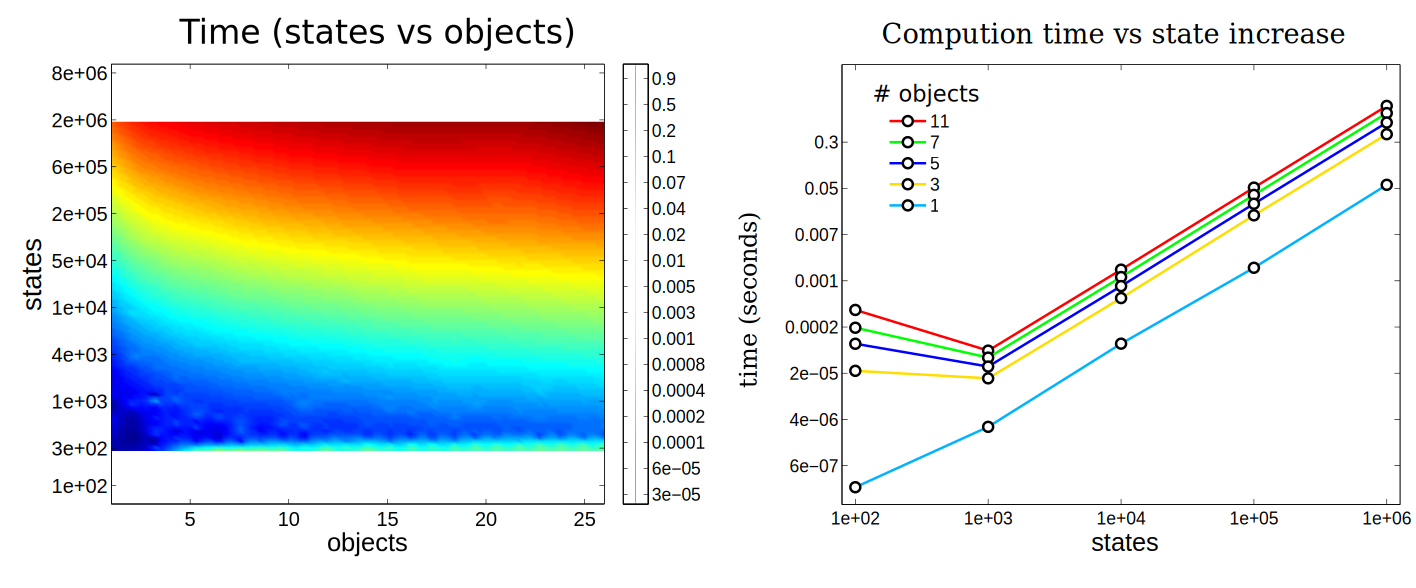
\includegraphics[width=\textwidth]{./ch5-MLMF/Figures/Figure12_v2.pdf}
 \caption{\textbf{Time complexity:} \textit{left:} mean time taken for a loop update (motion and measurement) as a function of the number of states in a marginal and the 
 number of objects present. \textit{right:} time taken for a loop update with respect to the number of states in the marginal. The colour coded lines are 
 associated with the number of objects present. The computational cost is plotted on a log scale. As the number of states increases exponentially the
 computational cost matches it.}
 \label{fig:time_complexity}
\end{figure}


\subsection{Evaluation of independence assumption}\label{subsec:eval_indep_assumptiom}

In section \ref{subsec:scalabe_extension} we made the assumption (for scalability reasons) that the objects' beliefs are independent
from one another. To evaluate this assumption we compared our filter on three random variables, an agent and two objects with respect to the ground truth
which we obtain from the standard histogram filter. For each of the three beliefs (the agent and two objects), 100 different marginals 
were generated and the true locations (actual position of the agent and objects) were sampled from them. 
The agent carries out  a sweep of the state space for each of the 100 initialisations and the actual policy is saved 
and run with the scaled-MLMF filter. In the first experiment we assume that the objects are completely independent 
and that there is no transfer of information between the pair-wise joint distributions. In the second and third experiments we perform the exchange of information as 
described in Algorithm \ref{alg:scalabe-mrf-slam}. Here we compare the effect of using the product of the agent's marginals $P(A_t|Y_{0:t}) = P(A^{(1)}_t|Y^{(1)}_{0:t}) \cdot P(A^{(2)}_t|Y^{(2)}_{0:t})$ 
against their average $P(A_t|Y_{0:t}) = \frac{1}{2}P(A^{(1)}_t|Y^{(1)}_{0:t}) + \frac{1}{2}P(A^{(2)}_t|Y^{(2)}_{0:t})$. 

For each of the 100 sweeps we compared the ground truth given by the histogram filter and scalabe-MLMF using the Hellinger distance (Equation \ref{eq:hellinger}).
\begin{equation} \label{eq:hellinger}
 H(P,Q) = \frac{1}{\sqrt{2}}\, \|\sqrt{P} - \sqrt{Q}\|_2  
\end{equation}
The Hellinger distance is a metric which measures the distance between two probability distributions. Its value lies strictly between 0 (the two 
distributions are identical) and 1 (no overlap between them). Figure \ref{fig:independence_assumption_test} shows the kernel density 
distribution of the Hellinger distances taken at each time step for all 100 sweeps.

The best results were for case 3). The \textit{bottom plots} show that the Hellinger distance distribution between the
object marginals for both case 2) and 3) are the same. However there is a significant improvement when using the average of the agent's marginals as oppose to 
their product. 

\begin{figure}
 \includegraphics[width=\textwidth]{./ch5-MLMF/Figures/Figure13.pdf}
 \caption{\textbf{Comparison of scalable-MLMF and the histogram filter} A deterministic sweep policy was carried out for 100 different initialisations of 
 the agent and object beliefs. \textit{top left:} One particular Initialisation of the agent and object
 random variables. The true position of the agent and objects were sampled at random. The black arrow indicates the general policy which was 
 followed for each of the 100 sweeps. 
 These were performed for 1) scalable-MLMF  with objects considered to be independent at all times (no Algorithm \ref{alg:scalabe-mrf-slam}). 2) 
 Agent marginal $P(A_t|Y_{0:t})$ is the product of marginals $P(A^{(i)}_t|Y^{(i)}_{0:t})$ (Equation \ref{eq:marg_indep_prod}). 
 3) marginal $P(A_t|Y_t)$ is taken to be the average 
 of all marginals $P(A^{(i)}_t|Y^{(i)}_{0:t})$ (Equation \ref{eq:marg_indep_sum}).  For each of these three experiment we report the 
 kernel density estimation over the Hellinger distances taken at every time step between ground truth (from histogram filter) and scalable-MLMF.}
 \label{fig:independence_assumption_test}
\end{figure}

\subsection{Evaluation of memory}

The memory is the list of all measurement likelihood functions which have been applied on the joint 
distribution since initialisation. As detailed previously there can be no more than $N$ different measurement likelihood functions added to 
memory. In the case of a very large state space this might be cumbersome. We investigate how restricting the memory size 
can impact on the decision process in an Active-SLAM setting. Given our set up we choose a breadth-first search in the action 
space with a one time step horizon, making it a greedy algorithm. The objective function we utilise is the information
gain of the beliefs after applying an action (Equation \ref{eq:greedy_algorithm}).

\begin{equation}\label{eq:greedy_algorithm}
 u_{t} = \operatorname*{arg\,max}_{u_t} H\{P(A_{t-1},O|Y_{0:t-1},u_{0:t-1})\} - \mathbb{E}_{Y_t}\left[H\{P(A_{t},O|Y_{0:t},u_{0:t})\}\right]
\end{equation}

For each action we run the filter forward in time and sample from the measurement model since we cannot know ahead of time the actual 
measurement and have to estimate it. The information gain is the difference between the current entropy (defined 
by $H\{\cdot\}$) and the future entropy after the simulated motion and measurement update. The action with the highest information gain 
is subsequently selected. This is repeated at each time step. In Figure \ref{fig:exploration_init} we illustrate the environment setup for 
a 1D and 2D case. The agent's task is to find the objects in the environment.


\begin{figure}
  \includegraphics[width=\textwidth]{./ch5-MLMF/Figures/Figure14.pdf}
  \caption{\textbf{Agent's prior beliefs.} Two types of environment, the first is 
  a 2D world in which the agent lives in a square surrounded by a wall whilst the second is a 1D
  world. In the 2D figures the agent is illustrated by a circle with a bar to indicate its heading. The true location 
  of the objects are represented by colour coded squares. \textit{Top row} three different initialisations of the agent's location. 
  \textit{Bottom row} d) the agent's prior beliefs with respect to the location of the first object and e) belief of the second object's location.
  \textit{bottom row} f) 1D world with one object.}
  \label{fig:exploration_init}
\end{figure}

For the 2D search we consider three different initialisations (single-Gaussian, four-Gaussian, Uniform) for the agent's belief where there are 
two objects to be found. Ten searches were carried out for each of the three initialisations of the agent's beliefs. 
The true location of the agent, for each search, is sampled from its initial belief and the objects' locations 
(red and green squares in Figure \ref{fig:exploration_init}) are kept fixed throughout all searches. We repeat each search for 18 different memory 
sizes going from 1 to $N$ (the number of states). For the 1D search case we consider 1 object since adding more objects will make the search easier. 
We are interested in how the memory effects the search and not the search itself. In Figure \ref{fig:time_to_reach_goal} we report on the time taken to 
find all objects with respect to a given memory size which is shown as the percentage of the total number of states. 
In the 1D search case the variability of time taken to find the object converges when the memory size is at 60\% of the original state space. 
As for the 2D search with 2 beliefs (agent \& 1 object) the convergence depends on the agent's initial belief. For the 1-Gaussian (green line) 
all searches take approximately the same amount of time after a memory size of 9\%. As for the remaining two initialisations convergence is achieved at  48\%. 
The same holds true for the case of 3 beliefs (agent \& 2 objects).

In the 2D searches, the size of the memory has a less drastic impact than in the 1D (which is a special search case). 
In the 2D case only when the memory size is less than 6\% is there a significant impact in terms of the time taken to find 
the objects. We conclude that at least in the case of the greedy one step-look ahead planner which is frequently used in the literature, the 
size of the memory seems not to be a limiting factor in terms of the time taken to accomplish the search.


\begin{figure}
  \includegraphics[width=\textwidth]{./ch5-MLMF/Figures/Figure15.pdf}
  \caption{\textbf{Memory size vs time to find objects} Results of the effect of the memory size on the decision process.
  The memory size is reported as the percentage of total number of states present in the marginal space. At 100\% the size
  of the memory is equal to that of the state space. \textit{left:} results of the 1D search illustrated in Figure \ref{fig:exploration_init} \textit{f)}.
  \textit{Middle \& right:} 2D search with initialisations accordingly depicted in Figure \ref{fig:exploration_init}.
  }
  \label{fig:time_to_reach_goal}
\end{figure}

\FloatBarrier
\section{Conclusion}\label{ch5:conclusion}

This work addresses the Active-SLAM filtering problem for scenarios in which sensory information relating to the map is very limited. Current
SLAM algorithms filter the errors originating from sensory measurements and not prior uncertainty. By making the assumption
that the joint distribution of all the random variables is a multivariate Gaussian, inference is tractable. Since the origin of 
our uncertainty is not originating from the measurement noise we cannot assume the joint distribution to have any special structure. 
A suitable filter for such purposes is the histogram which makes no assumption about the shape or form the joint distribution might take. 
The drawback of this form of parametrisation is that the space and time complexity is exponential with respect to the number of states and random variables 
and is a major limiting factor for scalability. 

The main contribution of this work is a formulation of a histogram Bayesian state space estimator in which the computational complexity is 
both linear in time and space. We took a different approach to other SLAM formulations in the sense that we did not
explicitly parametrise the joint distribution but kept all parametrisation in the space of the marginals (beliefs),
avoiding the exponential increase in parameter space which would otherwise have been the case. Our filter's parameters 
consist of the marginals and the history of measurement functions which have been applied. By evaluating the joint 
distribution solely at the states which are affected by the current measurement function whilst taking into account the 
memory, the MLMF filter can recover exactly the same filtered marginals as the histogram filter. The worst case space complexity is 
linear rather than exponential and the time complexity remains exponential but grows at a slower rate than in the histogram filter.
In the striving to make the filter scalable we introduced an independence assumption between the objects. An individual MLMF filter
was used for each agent-object pair. We evaluated the difference between the scalable-MLMF filter with a ground truth provided 
by the histogram filter for 100 different searches with respect to the Hellinger distance between them. We concluded that 
the divergence was relatively small and thus the scalable-MLMF filter provides a good approximation to the true filtered
marginals. We evaluated the time taken to perform a motion-update loop for different discretisation of the state space (100 to 10'000'000 states) and 
number of objects (2 to 25) present. In most of the cases we achieved an update cycle rate below 1Hz. We evaluated how the increase of the number of states 
effected the computational cost. The relationship was found to be linear and thus is in agreement with our analysis of the asymptotic growth rate. 
We analysed the effect the memory size (the remembered number of measurement likelihood functions) has on the decision theoretic process of reducing
the uncertainty of the map and agent during a search task. We found that in the 2D case the memory size has much less of an effect that in the 1D case
and we conclude that it is unnecessary to remember every single measurement function.

The implications of the MLMF and scalable-MLMF filter is that we have a computationally tractable means of 
performing SLAM in a case scenario where a lot of negative information is present and  we cannot assume the 
joint distribution has any specific structure. The filter can be used at higher cognitive level than 
processing raw sensory information as it is often in Active-SLAM. It would be well suited for reasoning about belief 
of location of objects in a setting where the robot's field of view is limited.

An interesting future extension is to make the original MLMF filter scalable without introducing assumptions.
One possibility would be to consider Monte Carlo integration methods for inference. These can scale well to high dimensional 
spaces whilst still providing reliable estimates. A second aspect would be to investigate the possibility
of using Gaussian Mixtures as a form of parametrisation of the marginals so that it might be possible to blend our filter with  
EKF-SLAM. This would allow the parameters to grow quadratically with respect to the dimension of the marginal space as opposed to
exponentially as it is in the case with the histogram and MLMF filters.



\section{Appendix}\label{ch5:appendix}

%\subsection{EKF-SLAM models}
%\paragraph{Motion update}
%\begin{align}
%  \bar{\mu}_t      &= f(\mu_{t-1},u_t)\\
%  \bar{\Sigma}_{t} &= F \Sigma_{t-1} F^{\mathrm{T}} + Q
%\end{align}
%Where $F = \left[\frac{\partial f(\mu_{t-1},u_t)}{\partial \mu_{t-1} } \right]$ is the Jacobian of the dynamic model with respect to the Gaussian mean. The 
%bar notation on the mean and covariance is to indicate that no sensing information has been used to update their estimates.
%\paragraph{Measurement update}
%\begin{align}
%   K    &= \bar{\Sigma}_{t} H (H \bar{\Sigma}_{t} H + R)^{-1} \\
%  \mu_t &= \bar{\mu}_t + K \cdot (Y_t - \hat{Y}_t)\\
%  \Sigma_t &= (I - KH) \bar{\Sigma}_{t}
%\end{align}
%Where $H = \left[\frac{\partial h(\mu_A,\mu_O;\beta)}{\partial \mu_A\mu_O}\right]$ is the Jacobian of the measurement function (Equation \ref{eq:ekf-measurement_function})  
%with respect to the mean of the joint distribution. 

%\subsection{Bayesian joint to filter}\label{appendix:bayes_joint}
%\begin{align}
%&P(A_t,O,Y_{0:t},u_{0:t})\\
%&= P(O) \left( \sum_{A_{0:t-1}}  P(A_0) \prod_{t=0}^{t} P(A_t|A_{t-1},u_{t}) P(Y_t|A_t,O) \right)  P(Y_t|A_t,O) \\
%&= P(O) \left( \sum_{A_{0:t-1}} P(A_{0:t},Y_{0:t-1},u_{0:t}) \right)  \\
%&= P(O) P(A_t,Y_{0:t},u_{0:t}) \\
%&= P(A_t,O,Y_{0:t},u_{0:t})
%\end{align}

\subsection{Bayesian filtering recursion}\label{appendix:bayes_recursion}

\paragraph{Joint distribution}\\
\begin{equation}
 P(A_{0:t},O,Y_{0:t}|u_{0:t}) = P(A_0)P(O)\prod_{t=1}^t P(A_t|A_{t-1},u_{t}) P(Y_t|A_t,O)
\end{equation}
\begin{equation}
  P(A_t,O,Y_{0:t}|u_{0:t}) = \sum_{A_{0:t-1}}  P(A_t,A_{0:t-1},O,Y_{0:t}|u_{0:t}) \\
\end{equation}


%  P(A_{0:t},O,Y_{0:t},u_{0:t})  &= P(A_0)P(O)\prod_{t=1}^{t} P(A_t|A_{t-1},u_{t-1}) P(Y_t|A_t,O) \\
\paragraph{Filtering problem}\\
We derive $P(A_t,O|Y_{0:t},u_{0:t})$, we start from the joint distribution, Equation \ref{eq:br_chain}:
\begin{equation}
   P(A_t,O,Y_{0:t}|u_{0:t})  = \sum_{A_{t-1}} P(A_t,A_{t-1},O,Y_t,Y_{0:t-1}|u_{t},u_{0:t-1}) \label{eq:br_chain} 
\end{equation}


\begin{tabular}{lll}
   $P(A_t,O,Y_{0:t}|u_{0:t})$ & $=\sum_{A_{t-1}}$ &  $P(Y_t|\Ccancel[red]{Y_{0:t-1}},A_t,\cancel{A_{t-1}},O,\cancel{u_{t}},\cancel{u_{0:t-1}}) $ \\
			      &  & $P(A_t|A_{t-1},\Ccancel[red]{O},u_{t},\Ccancel[red]{Y_{0:t-1}},\Ccancel[red]{u_{0:t-1}}) $ \\
			      &  & $P( A_{t-1},O,Y_{0:t-1}|\Ccancel[red]{u_t},u_{0:t-1})$
\end{tabular}

\begin{align}
  &P(A_t,O,Y_{0:t}|u_{0:t}) \\
  &= \sum_{A_{t-1}} P(Y_t|A_{t},O)  P(A_t|A_{t-1},u_{t})  P(A_{t-1},O,Y_{0:t-1}|u_{0:t-1}) \nonumber \\
  &= P(Y_t|A_{t},O)  \underbrace{\sum_{A_{t-1}} P(A_t|A_{t-1},u_t)  P(A_{t-1},O,Y_{0:t-1}|u_{0:t-1})}_{P(A_t,O,Y_{0:t-1}|u_{0:t})} 
\end{align}

\begin{align}
   P(A_t,O,Y_{0:t}|u_{0:t}) &= P(Y_t|A_{t},O)  P(A_t,O,Y_{0:t-1}|u_{0:t}) \nonumber \\
			    &= P(Y_t|A_{t},O)  P(A_t,O|Y_{0:t-1},u_{0:t})  P(Y_{0:t-1}|u_{0:t})
\end{align}


%From line \ref{eq:br_chain} to \ref{eq:cancellations} we apply the chain rule of probabilities.
All the cancellations come from the \textit{Markov Assumption} read from the structure of the Bayesian network.
The resulting final Bayesian recursion is obtained by conditioning on the measurement and actions, which is the normalisation factor.

\begin{align}\label{eq:ch5_measurement_update}
 P(A_t,O|Y_{0:t},u_{0:t}) &= \frac{P(Y_t|A_{t},O)  P(A_t,O|Y_{0:t-1},u_{0:t})  P(Y_{0:t-1}|u_{0:t})}{P(Y_{0:t}|u_{0:t})} \nonumber \\
			  &= \frac{P(Y_t|A_{t},O)  P(A_t,O|Y_{0:t-1},u_{0:t})  \Ccancel[red]{P(Y_{0:t-1},u_{0:t})}}{P(Y_t|Y_{0:t-1},u_{0:t}) \Ccancel[red]{P(Y_{0:t-1}|u_{0:t})}}  
\end{align}
 
\begin{equation}
   P(A_t,O|Y_{0:t},u_{0:t}) = \frac{P(Y_t|A_{t},O) P(A_{t},O|Y_{0:t-1},u_{0:t})}{P(Y_t|Y_{0:t-1},u_{0:t})} 
\end{equation}


\begin{align}
 P(Y_t|Y_{0:t-1},u_{0:t}) &= \sum\limits_{A_t} \sum\limits_O  P(Y_t|A_{t},O) P(A_{t},O|Y_{0:t-1},u_{0:t}) \\
			  &= \sum\limits_{A_t} \sum\limits_O  P(Y_t,A_{t},O|Y_{0:t-1},u_{0:t})
\end{align}

\subsection{Recursion example}


\begin{align}
  P(A_0,O)     &= P(O) P(A_0)\\
  P(A_0,O,Y_0) &= P(O) P(A_0) P(Y_0|A_0,O) \\
  P(A_1,O,Y_0|u_1) &= P(O)\sum\limits_{A_0} P(A_1|A_0,u_1) P(A_0) P(Y_0|A_0,O)\\
                   &= P(O)\sum\limits_{A_0} P(A_1,A_0,Y_0|u_1,O)\\
                   &= P(O) P(A_1,Y_0|u_1,O)\\
                   &= P(O) P(A_1|u_1) P(Y_0|A_1,O)
\end{align} 

\begin{align}
 &P(A_2,O,Y_{0:1}|u_{1:2}) = \nonumber \\
 &P(O) \sum\limits_{A_1} P(A_2|A_1,u_2) P(A_1) P(Y_0|A_1,O,u_1) P(Y_1|A_1,O) = \\
 &P(O) \sum\limits_{A_1} P(A_2,A_1|u_2) P(Y_0|A_1,O,u_1) P(Y_1|A_1,O) \\
 &P(O) P(A_2|u_{1:2}) P(Y_0|A_2,O) P(Y_1|A_2,O)
\end{align}



\subsection{Derivation of the evidence}\label{appendix:evidence}

From first principle, Equation \ref{eq:marginal_likelihood_memory}, we demonstrated that the marginal likelihood (also called evidence) is simply the difference
in the probability mass located inside the measurement functions after applying $P(Y_t|A_t,O)$.

The marginal likelihood is the marginalisation of all non measurement random variables from 
the nominator of Equation \ref{eq:ch5_measurement_update} \& \ref{eq:ch5:numerator} (we dropped $u_{0:t-1}$ for easing the notation).
\begin{align}\label{eq:ch5:numerator}
  P(A_t,O,Y_t|Y_{0:t-1}) &= P(Y_t|A_t,O) \cdot P(A_t,O|Y_{0:t-1})\\ 
 P(Y_t|Y_{0:t-1}) &= \sum\limits_{A_t}\sum\limits_{O} P(Y_t,A_t,O|Y_{0:t-1})  \label{eq:marginal_likelihood_memory}  
\end{align}
 
\begin{align}
 &P(Y_t|Y_{0:t-1}) \\ 
		  &= \sum\limits_{A_t}\sum\limits_{O} P(Y_t|A_t,O)\cdot P(A_t,O|Y_{0:t-1}) \\
		  &= \sum\limits_{A_t}\sum\limits_{O} P(Y_t|A_t,O)\cdot \Big(P_{\ominus}(A_t,O|{\color{red}Y_{0:t-1}}) + P_{\cap}(A_t,O|Y_{0:t-1})\Big)\\
		  &= \sum\limits_{A_t}\sum\limits_{O} P_{\ominus}(A_t,O|{\color{red}Y_{0:t}}) + P(Y_t|A_t,O)\cdot P_{\cap}(A_t,O|Y_{0:t-1}) \label{eq:marginal_likelihood_memory_last}
\end{align}

In Equation \ref{eq:ch5:less1_1}, we use the fact that after applying the measurement likelihood function, which lies in the interval $0 \leq P(Y_t|A_t,O) \leq 1$, 
to the joint distribution, its sum will always be smaller or equal to $1$.
From Equation \ref{eq:ch5:less1_1} to \ref{eq:ch5:less1_2} we use the fact that $P(A_t,O|Y_{0:t-1})$ is a probability density and must sum to 1.

\begin{align}
  \sum\limits_{A_t}\sum\limits_{O} P(Y_t|A_t,O) \cdot P(A_t,O|Y_{0:t-1})  &\leq \sum\limits_{A_t}\sum\limits_{O} P(A_t,O|Y_{0:t-1}) \label{eq:ch5:less1_1}\\
  \sum\limits_{A_t}\sum\limits_{O} P(Y_t|A_t,O) \cdot P(A_t,O|Y_{0:t-1}) &\leq 1 \label{eq:ch5:less1_2} \\
  P(Y_t|Y_{0:t-1}) &\leq 1 \\
  P(Y_t|Y_{0:t-1}) + \alpha &= 1 \label{eq:marginal_likelihood_equal_I}
\end{align}
We equate Equation \ref{eq:marginal_likelihood_equal_I} with \ref{eq:marginal_likelihood_memory_last} and find a solution for the marginal likelihood which
only depends on areas of the joint distribution which are dependent.
		   
\begin{align}		  
 &\overbrace{\sum\limits_{A_t}\sum\limits_{O} P(A_t,O|Y_{0:t-1})}^{=1} - \alpha  = \nonumber \\ 
      &\sum\limits_{A_t}\sum\limits_{O} P_{\ominus}(A_t,O|Y_{0:t}) + P(Y_t|A_t,O)\cdot P_{\cap}(A_t,O|Y_{0:t-1})
\end{align}

\begin{align}   
   \alpha &= \sum\limits_{A_t}\sum\limits_{O}  \overbrace{P_{\ominus}(A_t,O|Y_{0:t}) + P_{\cap}(A_t,O|Y_{0:t-1})}^{P(A_t,O|Y_{0:t-1})}\nonumber\\ 
     & - P_{\ominus}(A_t,O|Y_{0:t}) - P(Y_t|A_t,O)\cdot P_{\cap}(A_t,O|Y_{0:t-1}) \\
    \alpha &= \sum\limits_{A_t}\sum\limits_{O} P_{\cap}(A_t,O|Y_{0:t-1}) - P(Y_t|A_t,O)\cdot P_{\cap}(A_t,O|Y_{0:t-1}) \\
	   &= \sum\limits_{A_t}\sum\limits_{O} P_{\cap}(A_t,O|Y_{0:t-1}) (1 - P(Y_t|A_t,O)) \label{eq:marginal_likelihood_equal_I2}
\end{align}

The last line, Equation \ref{eq:marginal_likelihood_equal_I2}, when substituted back into line \ref{eq:marginal_likelihood_equal_I}, tells us that the 
normalisation factor or marginal likelihood is $1$ minus the difference in the area of dependence a priori to the application of 
the measurement function, Equation \ref{eq:marginal_liklihood_final}.

\begin{equation}\label{eq:marginal_liklihood_final}
 P(Y_t|Y_{0:t}) = 1 - \alpha
\end{equation}


\subsection{Derivation of the marginal}\label{appendix:marginal}

The marginal of a random variable is the marginalisation or integration over all other random variables, $P(A_t,|Y_{0:t}) = \sum\limits_{O} P(A_t,O|Y_{0:t})$. Below 
we give a form of this integration which exploits the independent regions in the joint distribution.

\begin{equation} \label{eq:ch5:app:dummy}
 P(A_t,|Y_{0:t}) = \mathbf{P(A_t|Y_{0:t-1})} - \Big(\mathbf{P(A_t|Y_{0:t-1})} - P(A_t|Y_{0:t}) \Big) 
\end{equation}

In Equation \ref{eq:ch5:app:dummy} we add and substract $P(A_t|Y_{0:t-1})$ and we further split 
$P(A_t|Y_{0:t-1})$ into independent and dependent components: 

\begin{align}
  &P(A_t,|Y_{0:t}) =  P(A_t|Y_{0:t-1}) - \nonumber \\ 
  &\Big(\underbrace{P_{\cap}(A_t|Y_{0:t-1}) + \Ccancel[red]{P_{\ominus}(A_t|Y_{0:t-1})}}_{P(A_t|Y_{0:t-1})} -  \underbrace{P_{\cap}(A_t|Y_{0:t}) + \Ccancel[red]{P_{\ominus}(A_t|Y_{0:t})}}_{P(A_t|Y_{0:t})})   \Big) \label{eq:dependence1} 
\end{align}
From equation \ref{eq:dependence1} to \ref{eq:dependence2} we used the fact that independent regions of the marginal distributions will remain unchanged after
an observation, $P_{\ominus}(A_t|Y_{0:t-1}) = P_{\ominus}(A_t|Y_{0:t})$, and before re-normalisation. This results in the final recursive update:
\begin{equation}
 P(A_t,|Y_{0:\color{red}{t}}) =  P(A_t|Y_{0:\color{red}{t-1}}) - \Big(P_{\cap}(A_t|Y_{0:t-1}) -  P_{\cap}(A_t|Y_{0:t})  \Big) \label{eq:dependence2} 
\end{equation}
Equation \ref{eq:dependence2} states that only elements of the marginals which are dependent will change by the difference of before and after 
a measurement update.


%\subsection{Space \& time complexity (scalable-MLMF)}\label{appendix:space_time_scalable_mlmf}
%\subsection{Space complexity}
%\paragraph{Scalable-MLMF}
%The initial number of parameters is $\left(M - 1\right) \cdot \left(2 \cdot (2 \cdot N)\right)$. The $(2 \cdot N)$ is the cost per random variable
%as before, the additional factor of $2$ arises because we model pair-wise joint distributions and there are two random variables per joint distribution. The final
%factor $\left(M - 1\right)$ corresponds to the total number of joint distributions, in the case of $M$ random variables. The final cost is then 
%$(M - 1) \cdot N \cdot \left(4 + D\right)$ when taking into account the history.
%\subsection{Time complexity}
%\paragraph{Scalabe-MLMF} The computational cost is $\BigO{2 \cdot \left(M - 1\right) \cdot N }$. For one agent-object joint distribution, $N$
%states lie in the area of influence of the measurement function. Given $M$ random variables, the number of states needed to evaluate in all the joint distributions
%is $M-1$. The final marginal of the agent $P(A_t|Y_t) = \prod\limits_{i=1}^{M-1} P(A^{(i)}_t|Y^{(i)}_t)$ is obtained through $(M-1)\cdot N$ multiplications or additions.
%This explains the factor of $2$ in the final computational cost.
%\paragraph{Memory}\label{appendix:memory_time_complexity}%
%The MLMF filter stores the history of all likelihood functions which have been applied on the joint distribution. This is the 
%memory term $P(Y_{0:t-1}|A_t,O)$ in Equation \ref{eq:joint_filter_memory}. Table \ref{tab:memory_list} shows the memory list after three 
%iterations and the resulting effect in  the joint distribution is illustrated in Figure \ref{fig:3bel_lik_profile} \textit{right}.
%\begin{table}
%\begin{center}
% \begin{tabular}{llc}
% $P(Y_{0 }|A_0,O)  = $  & $P(Y_0|A_0,O)$				                            & (t=0) \\
% $P(Y_{0:1}|A_1,O) = $  & $P(Y_1|A_1,O) \cdot P(Y_0|A_1,O+u_1)$                             & (t=1) \\
% $P(Y_{0:2}|A_2,O) = $  & $P(Y_2|A_2,O) \cdot P(Y_1|A_2,O+u_1) \cdot P(Y_0|A_2,O+u_1+u_2)$  & (t=2)
%\end{tabular}
%\end{center}
%\caption{\textbf{Memory list} After three updates the memory term $P(Y_{0:t}|A_t,O)$ contains three functions. The parametrisation
%of the functions is the same with the exception of actions $u_t$ which are added after each motion update step. As the result the 
%first function added to the list will have all the actions applied to it from the first time step to the last.}
%\label{tab:memory_list}
%\end{table}

%At every time step the current action (causing a displacement) is applied to all elements in the memory before appending the new 
%measurement function $P(Y_t|A_t,O)$. The application of the actions causes a shift of likelihood functions along the agent's axis
%in the joint distribution. As a result, the memory list is always sorted and the first element is always the last measurement function
%to have been applied. 
%During the measurement update Equation \ref{eq:marignal_mrf_2}, only the first entry of the memory function has to be evaluated
%giving a cost of $\BigO{1}$ at every time step when evaluating the dependent states (those which lie on the hyperplane). When
%evaluating a point which is not on the hyperplanes, its offset ($c$) can be evaluated $A=O+c$ and checked whether it is contained
%within the list. We employ a binary search which has a time complexity of $\BigO{\log(n)}$ (where $n$ is the current size of the memory). This is not necessary during most
%of the filtering process since the dependent states to be evaluated in the joint distribution always lie on the line $A=O$.
	 		\fi
\ifdefined	\gDisplayConclusions 		\chapter{Conclusion and summary}

\section{Main Contributions}

\section{Limitations and Future Work}

\section{Final Words}
  			\fi
\ifdefined	\gDisplayAppendix 	 	
\begin{appendices}

\chapter{Peg in hole}

\section{Time to connect socket}
\label{app:anova_socket}


We aim to test if there is any significant difference in time taken to connect socket A and B. We hypothesised that socket A requires longer time than socket B. 


Data from two groups of 5 subjects where collected according the the experiment protocol.
All subjects had time to familiarise themselves with the task and accomplished multiple training rounds 
before the start of the experiment.
In Figure \ref{figuretimesubgroup} (\textit{Top row}) we plot the time taken for each subject to connect the plug 
to the socket, once the socket was localised.
 
Before applying a statistical test to compare the time taken to connect the plug to the sockets for the 
two groups, we tested the normality of the time-distribution of each experiment condition (AA, AB, BA, BB).

We applied Shapiro-Wilk test of normality in R and used Q-Q plots to compare the shapes 
of distributions (Figure \ref{QQplot}) with normality. None of the time-distributions of the experimental conditions
are normal (p< 0.0001). Therefore, we chose a non-parametric test to compare the 
distributions. Since socket A and B were performed by related samples we applied the
Wilcoxon signed-rank test (a paired difference test). This test assesses whether the population mean rank differs 
between the two sockets (A and B) given that a subject performed both experiments one after the other.

Socket A took significantly longer time than socket B and this result was observed in the two 
groups (Group A p<0.0001, Group B p=0.0002, Wilcoxon signed-rank test, Figure \ref{figuretimesubgroup}).   


\begin{figure}
 \centering
 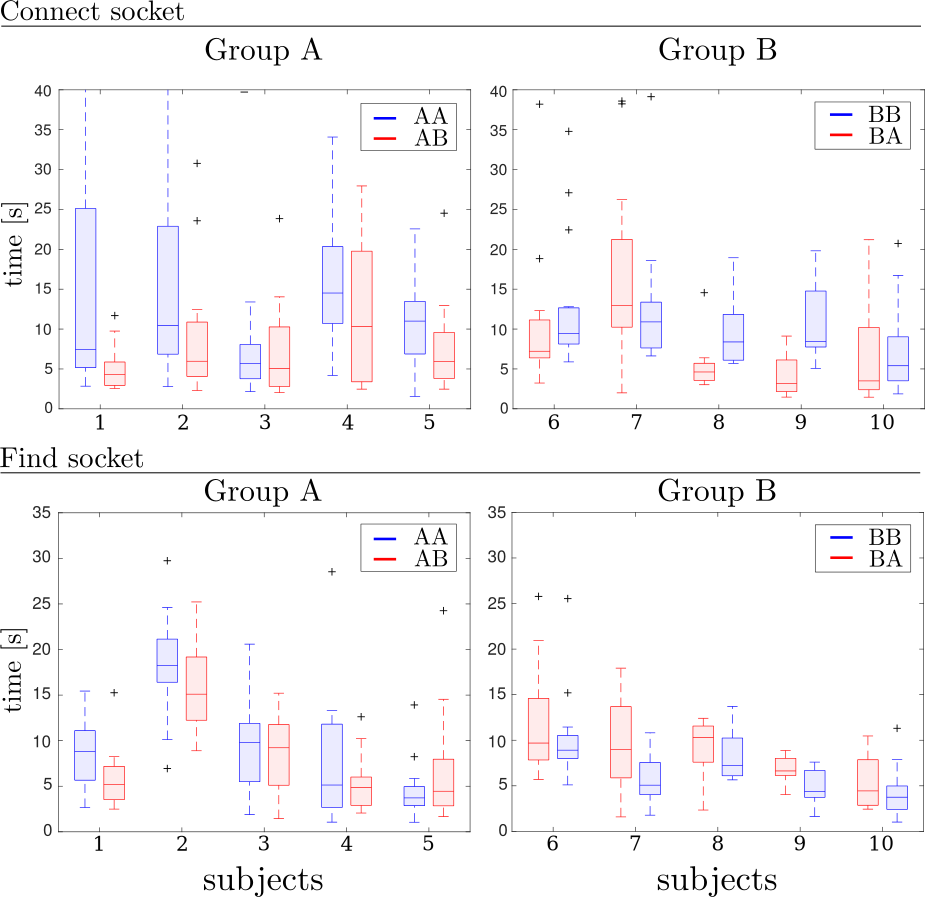
\includegraphics[width=\textwidth]{./ch4-PiH/Figures/time_taken_subgroup.pdf}
 \caption{Time taken to find and connect the plug to the power socket. \textbf{Top:} 
 Time taken to connect the plug to the socket once the socket is localised. For most subjects the median value of the taken time is higher 
 for socket A when compared with socket B. \textbf{Bottom}: time taken to localise the socket. For the second
 search, AB and BA, it seams that the subjects are faster indicating learning during the experiment.
 }
 \label{figuretimesubject}
\end{figure}

\begin{figure}	
   \centering
   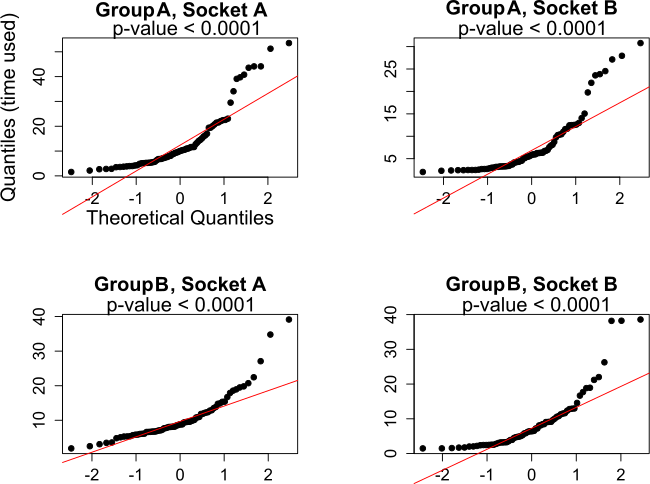
\includegraphics[width=0.9\textwidth]{./ch4-PiH/Figures/QQplot.pdf}
   \caption{Q-Q plots of time taken for four experiment conditions. The above p-values are from the Shapiro-Wilk test.}
   \label{QQplot}
\end{figure}


\begin{figure}
  \centering
  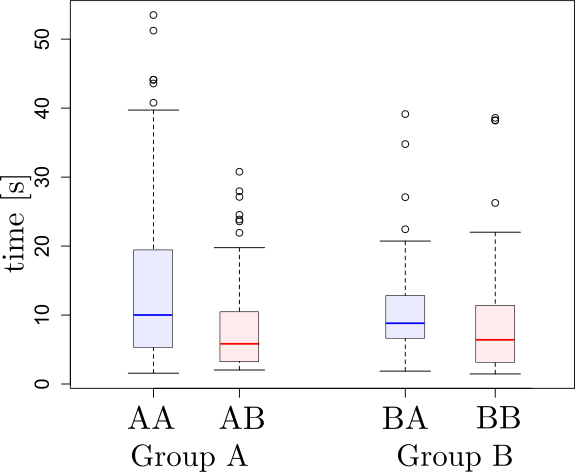
\includegraphics[width=0.8\textwidth]{./ch4-PiH/Figures/Group_Socket.pdf}
   \caption{Time taken to connect the sockets. For both groups, socket A always takes significantly longer time to connect, For Group A 
   p<0.0001 and for Group B p=0.0002.}
   \label{figuretimesubgroup}
\end{figure}

In summary, we observe that there is a significant effect of order. Starting with socket B greatly reduced the time 
taken for socket A (p=0.02). Regardless of the socket type between groups, the first socket always takes longer.
For AA vs BA, AA is significantly longer (p=0.02, Wilcoxon rank sum test). For socket B, BB vs AB, BB takes significantly
longer time (p<0.0001).


% 1) Is there are a difference across groups 
% 2) Is there a difference between the two sockets
%The null hypothesis is that there is no difference in the time taken to connect socket A or B. The result of the one-way anova
%is given in Table \ref{tab:ch4:anova_socket}. The null hypothesis is rejected at high significant level (***) indicating that 
%there is a difference between the sockets. According to the linear model it takes on average 4 seconds less to connect socket B 
%than it does for socket A.
%\begin{table}[h]
%\centering
%\begin{tabular}{lcc}
%  \hline
%          &   F    & Pr(>F)  	     \\ \hline
%   socket & 13.9   &  0.000232 *** 
%\end{tabular}
%\caption{One way anova of the time taken to connect two sockets A and B. There is a significant difference.}
%\label{tab:ch4:anova_socket}
%\end{table}
%We tested whether the group order had an effect on the connection time. We fitted a linear model
%with the predictor being time and the factors being the group (One or Two), the socket type (A or B) 
%and the subject's ID (1 to 10):
%\begin{equation}
% time = \beta_0 + \beta_1\, group + \beta_2\, socket + \beta_3\, subject
%\end{equation}
%and did the corresponding anova analysis on this linear model. We found that the difference between the sockets 
%remained significant.
\FloatBarrier
\section{EM policy search}\label{app:lb}
The objective of policy search in Reinforcement Learning (RL) is to optimise the parameters of a policy $\pi_{\Param}$
(which is a Gaussian Mixture Model (GMM) in our case) such to maximise a cost 
function, $J(\Param)$ Equation \ref{eq:ch4:app:J}, defined over the parameters of the policy:
%\begin{align}
%J(\Param)  &= \mathbb{E}_{\pi_{\Param}}\{R(\U,\B)\} \nonumber \\
%	   &= \sum\limits_{\B} d^{\pi}(\B) \sum\limits_{\U} \pi_{\Param}(\U,\B)\,R(\U,\B) \label{eq:ch4:app:J}
%\end{align}
%where $\B \sim d^{\pi}(\B)$ is the initial state distribution. The RL objective is to find a new set of parameters $\Param'$
%which maximises the above cost function $J$. Our approach follows the Monte-Carlo (MC) gradient estimate of Equation \ref{eq:ch4:app:J}
%through use of the log-likelihood ratio identity: $\nabla \log(\pi_{\Param}) = \nabla \pi_{\Param} / \pi_{\Param}$:


\begin{align}\label{eq:ch4:app:J}
 J(\Param) = \overbrace{\sum\limits_{i=1}^{N}   \underbrace{\left( \prod_{t=0}^{T^{[i]}} \pi_{\Param}(\U^{[i]}_t,\B^{[i]}_t) \right)}_{p_{\Param}(\tau_i)} \, R(\tau_i)}^{\mathbb{E}_{p_{\Param}}\{R\}} 
\end{align}

where $\tau_i = \{(\U_0,\B_0),\cdots,(\U_T^{[i]},\B_T^{[i]}) \}$ are the state-action samples of the $i$th episode. 
The total reward of one episode is the sum of discounted rewards:

\begin{equation}
 R(\tau_i) = \sum_{t=0}^{\mathrm{T^{[i]}}} \gamma^t \, r(\B^{[i]}_t,\U^{[i]}_t)
\end{equation}

where $\gamma \in [0,1)$ is the discount factor which dictates how much future rewards are considered important 
at the current decision point.
%\begin{align}
% \nabla_{\Param} J(\Param) &= \sum\limits_{\B} d^{\pi}(\B) \sum\limits_{\U}  \pi_{\Param}(\U,\B) \nabla_{\Param} \pi_{\Param}(\U,\B) \,R(\U,\B) \nonumber \\ 
%			   &= \mathbb{E}_{\pi_{\Param}}\{\nabla_{\Param} \log(\pi_{\Param}(\U,\B)) \,R(\U,\B)\} \label{eq:ch4:app:lJ}
%\end{align}
%This trick allows to evaluate the gradient of the parameters through Monte-Carlo trajectories generated from a the policy $\pi_{\Param}(\U,\B)$.
Most policy search methods are based gradient ascent on the cost function:
\begin{equation}
   \Param^{\mathrm{new}} =  \Param + \alpha\,\nabla_{\Param}J(\Param)
\end{equation}

The drawback of policy gradient methods is that a learning rate, $\alpha$, needs to be specified and the optimisation strongly depends 
on the fine tuning of this value. An alternative, which avoids
the learning rate problem, are Expectation-Maximisation (EM) methods. As our policy is a Gaussian Mixture Model (GMM) we can take advantage of 
the already existing EM updates of the GMM which are well known. Also updating the covariance parameters of the GMM by gradient ascent can lead 
to problems such the covariances being no longer positive-definite and this resolution requires the addition of constraints which becomes 
cumbersome. In contrast the EM solution for the GMM case is simple and easy to implement.

EM policy search methods have two phases. The first phase consists of generating a set of episodes $\boldsymbol{\tau}$ from 
the policy, this is the E-step. The second step consists of finding a new parameter $\Param^{\mathrm{new}}$ of the policy 
by maximising the cost function given the episodes:

\begin{equation}
  \Param^{\mathrm{new}} = \argmax\limits_{\Param} J(\Param) \label{eq:ch4:argmax}
\end{equation}

The above optimisation can be solved through the same approach taken in EM which consists of 
maximising the the logarithmic lower bound of the cost function $J(\Param)$: 

%The policy gradient theorem \cite{Sutton00policygradient} states the the gradient is:
%Steps taken to make a policy $\pi_{\Param}(\U,\B)$ maximise the objective function, .
%The policy will be maximised with respect to the lower bound of the cost function $J(\Param)$:
%\begin{align}
%  J(\Param') &= \sum_{i \in \mathbb{T}} \pi_{\Param'}(\Ui,\Bi)\, R(\Ui,\Bi) \nonumber\\ 
%	   &= \sum_{i \in \mathbb{T}}  \frac{\pi_{\Param'}(\Ui,\Bi)}{\pi_{\Param}(\Ui,\Bi)} \, \pi_{\Param}(\Ui,\Bi) \, R(\Ui,\Bi)
%\end{align}



\begin{align}
  \log( J(\Param) )  &= \log \sum\limits_{i=1}^{N} \frac{p_{\Param}(\tau_i)}{p_{\Param'}(\tau_i)} \, p_{\Param'}(\tau_i) \, R(\tau_i) \hspace*{2cm}  \nonumber \\
		     & \hspace*{2cm} \geq \underbrace{\sum\limits_{i=1}^{N} \log\Bigg( \frac{p_{\Param}(\tau_i)}{p_{\Param'}(\tau_i)}\Bigg) \, p_{\Param'}(\tau_i) \, R(\tau_i)}_{\mathcal{Q}(\Param,\Param')} \label{eq:lower_bound}
\end{align}
The parameter $\Param'$ belongs to the policy used to generate the episodes in the E-step and the parameter $\Param$ is the one 
we are optimising for. The lower bound $\mathcal{Q}(\Param,\Param')$ is derived from Jensen's inequality. 
The lower bound is next maximised by taking its derivative $\nabla_{\Param}\mathcal{Q}(\Param,\Param') = 0$. 
%We take the derivative of the lower bound of $\log(J(\Param'))$, Equation \ref{eq:lower_bound}, with respect to $\Param'$ and set it to 
%zero so as to maximise the cost function.

\begin{align}
 \nabla_{\Param}\mathcal{Q}(\Param,\Param')& = \sum\limits_{i=1}^{N} \nabla_{\Param} \log\big( p_{\Param}(\tau_i)\big) \, p_{\Param'}(\tau_i) \, R(\tau_i) - \hspace*{2cm} \nonumber \\
				    &\hspace*{2cm}\underbrace{\nabla_{\Param} \log\big( p_{\Param'}(\tau_i)\big)}_{=0} \, p_{\Param'}(\tau_i) \, R(\tau_i)				   
\end{align}
\begin{align}
 \nabla_{\Param}\mathcal{Q}(\Param,\Param') &= \mathbb{E}_{p_{\Param'}} \Big\{ \nabla_{\Param} \log\big( p_{\Param}(\tau_i)\big)\, R(\tau_i) \Big\} \label{eq:ch4:app:expec_Q}\\
					    &= \sum\limits_{i=1}^{N} \sum\limits_{t=0}^{T^{[i]}} \nabla_{\Param} \log\big( \pi_{\Param}(\Ui_t,\Bi_t)\big) \, R(\tau_i) \label{eq:ch4:app:logsum} \\
					    &= \sum\limits_{i=1}^{N} \sum\limits_{t=0}^{T^{[i]}} \nabla_{\Param}\log \pi_{\Param}(\U^{[i]}_t,\B^{[i]}_t) \, Q^{\pi_{\Param'}}(\U^{[i]}_t,\B^{[i]}_t) \label{eq:grad_log_cost_2}
\end{align}

From \ref{eq:ch4:app:expec_Q} to \ref{eq:ch4:app:logsum} we used the property: $\log( \prod \pi_{\Param} ) = \sum \log(\pi_{\Param})$ and 
the expectation vanishes as we evaluated it through sampling from the policy $\pi_{\Param'}$ (E-step). From \ref{eq:ch4:app:logsum} to \ref{eq:grad_log_cost_2} 
we used the fact that previous discounted rewards do not dependent on future time steps. The reader is referred 
to \cite[p. 50]{rl_gradient_survey_2013} for more details regarding Expectation-Maximisation and policy search in reinforcement learning.
In the next section \ref{app:grad} we maximise \ref{eq:grad_log_cost_2} for the case when the policy is parameterised by a GMM.


\section{Q-EM for GMM}\label{app:grad}

We derive the EM update rules of the lower bound $\mathcal{Q}(\Param,\Param')$ 
for a policy $\pi_{\Param}(\U,\B)$ parameterised by a Gaussian Mixture Model which we call 
Q-EM. Below we redefine the GMM function for convenience:

\begin{equation} \label{eq:ch5:app:gmm}
  \pi_{\Param}(\U,\B) = \sum\limits_{k=1}^K  \piK\,g(\U,\B;\MuK,\SigK)
\end{equation}

The parameters $\Param = \{w^{[k]},\MuK,\SigK\}_{1,\dots,K}$, are the weights, means and covariances 
of the individual Gaussian functions, $g(\cdot)$. 

Finding the new parameters of the GMM given a cost function $J(\Param)$ consists of maximising its logarithmic 
lower bound, Equation \ref{eq:ch4:app_div_Q}:

\begin{equation}\label{eq:ch4:app_div_Q}
  \nabla_{\Param}\mathcal{Q}(\Param,\Param') = \sum\limits_{i=1}^{N} \sum\limits_{t=0}^{T^{[i]}} \nabla_{\Param}\log \pi_{\Param}(\U^{[i]}_t,\B^{[i]}_t) \, Q^{\pi_{\Param'}}(\U^{[i]}_t,\B^{[i]}_t)
\end{equation}

As the ordering of the episode samples in the above equation does not mater we concatenate all the episodes into one dataset $\mathcal{D}$ 
and the $j$th sample in this dataset is given by $\mathbf{x}^{[j]} = [\U^{[j]},\B^{[j]}]^{\mathrm{T}}$. 

\begin{equation}\label{eq:ch4:app_div_Q_simple}
   \nabla_{\Param}\mathcal{Q}(\Param,\Param') = \sum\limits_{j=1}^{M} \nabla_{\Param}\log \pi_{\Param}(\mathbf{x}^{[j]}) \, Q^{\pi_{\Param'}}(\mathbf{x}^{[j]})
\end{equation}
To maximise Equation \ref{eq:ch4:app_div_Q_simple} we take the derivatives with respect to the 
parameters $\Param=\{w,\boldsymbol{\mu},\boldsymbol{\Sigma}\}$ of the GMM.  The reader my notice 
that the above equation is the derivative of the log-likelihood of the dataset $\mathcal{D}$ weighted
by $Q^{\pi_{\Param'}}$, a constant scalar value. As a consequence the result of maximisation will 
be similar to the standard EM solution of the GMM with an additional weighting factor. For a 
reference on the derivative of the log-likelihood of a GMM the reader is referred to \cite[p. 49]{matrix_ckb}
or \cite[Chap. 9]{Bishop_2006}.

%Setting the derivative of Equation \ref{eq:ch4:app_div_Q_simple} to zero and solving for the  
% we get a new weighted Maximisation update step in EM
%Making the substitution $\X = (\U,\B)^{\mathrm{T}}$ (small abuse of the notation) and  insuring a positive Q-function, $Q^{\pi}(\X^{[m]}) \geq 0$
%and by

\paragraph{Q-EM maximisation}

\begin{align}
    &\nabla_{\MuK} \mathcal{Q}(\MuK,\Param') =  \hspace*{5cm} \nonumber \\
    & \hspace*{1cm} \sum\limits_{j=1}^M \underbrace{\frac{\piK\,g(\Bx^{[j]};\MuK,\SigK)}{\sum\limits_{l=1}^{M} w^{[l]}\,g(\Bx;\Mu{l},\Sig{l}) } }_{\gamma_k(\Bx^{[j]})} \invSigK (\Bx^{[j]} - \MuK) \, \Qpx = 0 \label{eq:ch4:app:mu_max}
\end{align}

In \ref{eq:ch4:app:mu_max} we used the same notation and derivation as in \cite[Chap. 9.2.2]{Bishop_2006}, where $\gamma_k(\Bx^{[j]})$ is the responsibility factor, denoting 
the probability that data point $\mathbf{x}^{[j]}$ belongs to  Gaussian function $k$. After rearrangement the new mean is given by Equation \ref{eq:ch4:app_new_mu}.

\begin{empheq}[box={\tcbhighmath[colback=blue!2,colframe=blue]}]{align}
    \MuK_{\textrm{\textbf{new}}}    &= \frac{\sum\limits_{j=1}^{M} \gamma_k(\Bx^{[j]})\, \Qpx \, \Bx^{[j]} }{\sum\limits_{j=1}^{M} \gamma_k(\Bx^{[j]})\, \Qpx} \label{eq:ch4:app_new_mu} \\
    & \nonumber\\
    \SigK_{\textrm{\textbf{new}}}   &= \frac{\sum\limits_{j=1}^{M}  \gamma_k(\Bx^{[j]})\, \Qpx (\Bx^{[j]} - \MuK_{\textrm{\textbf{new}}})(\Bx^{[j]} - \MuK_{\textrm{\textbf{new}}})^{\mathrm{T}} }{ \sum\limits_{j=1}^{M} \gamma_k(\Bx^{[j]})\, \Qpx } \label{eq:ch4:app_new_cov}  \\
    & \nonumber\\
    w^{[k]}_{\textrm{\textbf{new}}} &= \frac{\sum\limits_{j=1}^{M} \Qpx \, \gamma_k(\Bx^{[j]})}{\sum\limits_{j=1}^{M} \Qpx} \label{eq:ch4:app_new_pi}
\end{empheq}

The covariances, Equation \ref{eq:ch4:app_new_cov}, and weights, Equation \ref{eq:ch4:app_new_pi}, are derived in a similar fashion.


\section{Unbiased estimator}\label{app:unbiased_delta}

%\begin{equation}
%  \delta^{\pi}_t = r_{t+1} + \gamma V^{\pi}(b_{t+1}) - V^{\pi}(b_t) \\
%\end{equation}
The temporal difference error is an unbiased estimate of the advantage function:
\begin{align}
  \displaystyle \mathop \mathbb{E}_{\pi_{\Param}} \{ \delta^{\pi}_t|b_t,u_t\} &=  \mathop\mathbb{E}_{\pi_{\Param}}\{ r_{t+1} + \gamma V^{\pi}(b_{t+1})|b_t,u_t\} - V^{\pi}(b_t) \nonumber \\
									   &= Q^{\pi}(b_t,u_t) - V^{\pi}(b_t) \nonumber \\
									   &= A^{\pi}(b_t,u_t)
\end{align}


\chapter{Non-parametric Bayesian State Space Estimator}\label{ch5:appendix}


\section{Probabilities}

There are two rules extensively used in the derivation of a Bayesian filter recursion regardless 
of the chosen parameterisation. Although well known we restate them here for convenience.

\begin{itemize}
 \item \textbf{Chain rule}\\
 \begin{equation}
  P(X_M,\cdots,X_1) = P(X_M|X_{M-1},\cdots,X_1) P(X_{M-1},\cdots,X_1) \label{eq:ch5:chain_rule}
 \end{equation}
 \item \textbf{Conditional independence}\\
  \begin{align}
    P(A,B|C) &= P(A|\Ccancel[red]{B},C) P(B|C) \nonumber \\
             &= P(A|C) P(B|C)
  \end{align}
  $A$ and $B$ are independent given that $C$ is known.
\end{itemize}


\section{Bayesian filtering recursion}\label{appendix:bayes_recursion}

\paragraph{Joint distribution}\\

The joint distribution is over all the random variables since $t=0$ until the current 
time step $t$:
\begin{align}
 &P(A_{0:t},O,Y_{0:t}|u_{1:t}) =\nonumber \\ 
 &P(A_0)P(O)P(Y_0|A_0,O)\prod_{t=1}^t P(A_t|A_{t-1},u_{t}) P(Y_t|A_t,O) \label{eq:ch5:app:joint} \\
 &P(A_0)P(O)P(Y_0|A_0,O) P(A_{1:t}|u_{1:t}) P(Y_{1:t}|A_{1:t},O)  \label{eq:ch5:app:joint_2} \\
 &P(A_0)P(O) P(A_{1:t}|u_{1:t}) P(Y_{0:t}|A_{0:t},O) \label{eq:ch5:joint_final}
\end{align}

From Equation \ref{eq:ch5:app:joint} to \ref{eq:ch5:app:joint_2} we made use of the chain rule 
of probabilities (Equation \ref{eq:ch5:chain_rule}) and the conditional independence $A_{t+1} \independent A_{t-1} | A_t$, see below a more concrete example for $P(A_{0:3}|u_{1:3})$:
\begin{align}
  &P(A_3,A_2,A_1,A_0|u_{1:3}) = \nonumber \\ 
  &P(A_3|A_2,\Ccancel[red]{A_1},\Ccancel[red]{A_0},u_{1:3})P(A_2|A_1,\Ccancel[red]{A_0},u_{1:3})P(A_1|A_0,u_{1:3}) P(A_0|u_{1:3}) = \label{eq:ch5:chain_example} \\
  &P(A_3|A_2,u_3,\Ccancel[red]{u_{1:2}})P(A_2|A_1,u_2,\Ccancel[red]{u_{1,3}})P(A_1|A_0,u_1,\Ccancel[red]{u_{2:3}}) P(A_0|\Ccancel[red]{u_{1:3}}) = \label{eq:ch5:cancel_actions} \\
  &\underbrace{(A_3|A_2,u_3) P(A_2|A_1,u_2) P(A_1|A_0,u_1)}_{P(A_{1:3}|u_{1:3})} P(A_0)
\end{align}

We applied the chain rule to get Equation \ref{eq:ch5:chain_example} and the cancellations arise from 
conditional independence between the agent random variable $A_t$ specified by the BN, 
see Figure \ref{fig:bayesian_sse_dag} on page \pageref{fig:bayesian_sse_dag}. The cancellations on line \ref{eq:ch5:cancel_actions}
arise also from BN, $A_t$ only depends on $u_t$ and no previous actions.


To see clearer the relationship between the left and right hand side of Equation \ref{eq:ch5:joint_final}, 
we can again apply the chain rule to the right, which gives:
\begin{align}
 P(A_{0:t},O,Y_{0:t}|u_{1:t}) &=  P(Y_{0:t}|A_{0:t},O,\Ccancel[red]{u_{1:t}}) P(A_{0:t},O|u_{1:t}) \\
			      &=  P(Y_{0:t}|A_{0:t},O) P(A_{0:t},O|u_{1:t})
\end{align}
The measurements $Y_{0:t}$ are independent of the actions $u_{0:t}$  given the history of the agent's random 
variables $A_{0:t}$. Next we see the relation between the thirst three terms on the right of Equation \ref{eq:ch5:joint_final}
with $P(A_{0:t},O|u_{1:t})$. We apply the chain rule:

\begin{align}
 P(A_{0:t},O|u_{1:t}) &= P(A_{0:t}|\Ccancel[red]{O},u_{1:t}) P(O|\Ccancel[red]{u_{1:t}}) \\
		      &= P(A_0) P(O) P(A_{1:t}|u_{1:t}) 
\end{align}

The object $O$ is conditionally independent of the actions and the second of actions $A_{0:t}$ are conditional independent 
of the object as they are dependent only on the measurements.

Typically we are interested in the filtered joint distribution $P(A_t,O,Y_{0:t}|u_{1:t})$ which 
is obtained by marginalising over $A_{0:t-1}$:
\begin{equation}
  P(A_t,O,Y_{0:t}|u_{1:t}) = \sum_{A_{0:t-1}}  P(A_t,A_{0:t-1},O,Y_{0:t}|u_{1:t}) \\
\end{equation}
A recursion exists making it not necessary to sum over all agents random variables from the state time 
until then end, but instead we only have to consider the last time step, see the next paragraph.

%  P(A_{0:t},O,Y_{0:t},u_{1:t})  &= P(A_0)P(O)\prod_{t=1}^{t} P(A_t|A_{t-1},u_{t-1}) P(Y_t|A_t,O) \\
\paragraph{Filtering problem}\\
We derive $P(A_t,O,Y_{0:t}|u_{1:t})$, we start from the joint distribution, Equation \ref{eq:br_chain}:
\begin{equation}
   P(A_t,O,Y_{0:t}|u_{1:t})  = \sum_{A_{t-1}} P(A_t,A_{t-1},O,Y_t,Y_{0:t-1}|u_{t},u_{1:t-1}) \label{eq:br_chain} 
\end{equation}

\begin{tabular}{lll}
   $P(A_t,O,Y_{0:t}|u_{1:t})$ & $=\sum_{A_{t-1}}$ &  $P(Y_t|\Ccancel[red]{Y_{0:t-1}},A_t,\cancel{A_{t-1}},O,\cancel{u_{t}},\cancel{u_{1:t-1}}) $ \\
			      &  & $P(A_t|A_{t-1},\Ccancel[red]{O},u_{t},\Ccancel[red]{Y_{0:t-1}},\Ccancel[red]{u_{1:t-1}}) $ \\
			      &  & $P( A_{t-1},O,Y_{0:t-1}|\Ccancel[red]{u_t},u_{1:t-1})$
\end{tabular}

\begin{align}
  &P(A_t,O,Y_{0:t}|u_{1:t}) \\
  &= \sum_{A_{t-1}} P(Y_t|A_{t},O)  P(A_t|A_{t-1},u_{t})  P(A_{t-1},O,Y_{0:t-1}|u_{1:t-1}) \nonumber \\
  &= P(Y_t|A_{t},O)  \underbrace{\sum_{A_{t-1}} P(A_t|A_{t-1},u_t)  P(A_{t-1},O,Y_{0:t-1}|u_{1:t-1})}_{P(A_t,O,Y_{0:t-1}|u_{1:t})} 
\end{align}

\begin{align}
   P(A_t,O,Y_{0:t}|u_{1:t}) &= P(Y_t|A_{t},O)  P(A_t,O,Y_{0:t-1}|u_{1:t}) \nonumber \\
			    &= P(Y_t|A_{t},O)  P(A_t,O|Y_{0:t-1},u_{1:t})  P(Y_{0:t-1}|u_{1:t})
\end{align}

All the cancellations come from the \textit{Markov Assumption} read from the structure of the Bayesian network.
The resulting final Bayesian recursion is obtained by conditioning on the measurement and actions, which is the normalisation factor.

\begin{align}\label{eq:ch5_measurement_update}
 P(A_t,O|Y_{0:t},u_{1:t}) &= \frac{P(Y_t|A_{t},O)  P(A_t,O|Y_{0:t-1},u_{1:t})  P(Y_{0:t-1}|u_{1:t})}{P(Y_{0:t}|u_{1:t})} \nonumber \\
			  &= \frac{P(Y_t|A_{t},O)  P(A_t,O|Y_{0:t-1},u_{1:t})  \Ccancel[red]{P(Y_{0:t-1},u_{1:t})}}{P(Y_t|Y_{0:t-1},u_{1:t}) \Ccancel[red]{P(Y_{0:t-1}|u_{1:t})}}   
\end{align}
 
\begin{equation}
   P(A_t,O|Y_{0:t},u_{1:t}) = \frac{P(Y_t|A_{t},O) P(A_{t},O|Y_{0:t-1},u_{1:t})}{P(Y_t|Y_{0:t-1},u_{1:t})} \label{eq:ch5:app:bayes_filter}
\end{equation}

The evidence is the the integration of all terms which are not measurements in the numerator of Equation \ref{eq:ch5:app:bayes_filter}.

\begin{align}
 P(Y_t|Y_{0:t-1},u_{1:t}) &= \sum\limits_{A_t} \sum\limits_O  P(Y_t|A_{t},O) P(A_{t},O|Y_{0:t-1},u_{1:t}) \\
			  &= \sum\limits_{A_t} \sum\limits_O  P(Y_t,A_{t},O|Y_{0:t-1},u_{1:t})
\end{align}
This is very expensive since we have to sum over the entire joint distribution, the MLMF avoids doing this by only considering the dependent 
regions of the joint distribution.

\section{Recursion example}\label{appendix:recursion_example}

Derivation of the filtered joint distribution, $P(A_t,O,Y_t|Y_{0:t},u_{1:t})$, for 
two updates. At initialisation when no action has yet been taken the filtered joint distribution 
is the product of the initial marginals and first likelihood function:
\begin{equation}
  P(A_0,O,Y_0) = P(O) P(A_0) P(Y_0|A_0,O) 
\end{equation}
  
The a first action, $u_1$ is applied, which to get the filtered joint distribution is marginalised:
\begin{align}
  P(A_1,O,Y_0|u_1) &= P(O)\sum\limits_{A_0} P(A_1|A_0,u_1) P(A_0) P(Y_0|A_0,O)\\
                   &= P(O)\sum\limits_{A_0} P(A_1,A_0,Y_0|u_1,O)\\
                   &= P(O) P(A_1,Y_0|u_1,O) \label{eq:ch5:rec_ex1}\\
                   &= P(O) P(Y_0|A_1,O,u_1) P(A_1|u_1,\Ccancel[red]{O}) \label{eq:ch5:rec_ex2}\\
                   &= P(O) P(Y_0|A_1,O,u_1) P(A_1|u_1) 
\end{align} 
From Equation \ref{eq:ch5:rec_ex1} to \ref{eq:ch5:rec_ex2} we used the Chain rule \ref{eq:ch5:chain_rule} and 
the cancellation in Equation \ref{eq:ch5:rec_ex2} arise from the factorisation of the joint distribution, 
see Figure \ref{fig:bayesian_sse_dag} on page \pageref{fig:bayesian_sse_dag}, $A$'s marginal does not depend on $O$.
After the application of the first action, the filtered joint has the following form:
\begin{equation}
 P(A_1,O,Y_0|u_1) = P(O) P(A_1|u_1) P(Y_0|A_1,O,u_1)
\end{equation}
A second measurement $Y_1$ and action $u_2$ are integrated into the filtered joint distribution:
\begin{align}
 &P(A_2,O,Y_{0:1}|u_{1:2}) = \nonumber \\
 &P(O) \sum\limits_{A_1} P(A_2|A_1,u_2) P(A_1|u_1) P(Y_0|A_1,O,u_1) P(Y_1|A_1,O) = \nonumber\\
 &P(O) \sum\limits_{A_1} P(A_2,A_1|u_{1:2}) P(Y_{0:1}|A_1,O,u_1) = \nonumber \\
 &P(O) \sum\limits_{A_1} P(A_2,A_1,Y_{0:1}|O,u_{1:2}) = \nonumber \\
 &P(O) P(A_2,Y_{0:1}|O,u_{1:2}) = \\
 &P(O) P(Y_{0:1}|A_2,O,u_{1:2})P(A_2|\Ccancel[red]{O},u_{1:2}) \label{eq:ch5:rec_ex3} 
\end{align}
We expand the function $P(Y_{0:1}|A_2,O,u_{1:2})$ to give a sense of how the likelihood function's positions 
get as illustrated in Figure \ref{fig:discrete_example} on page \pageref{fig:discrete_example}.

\begin{align}
  P(Y_0,Y_1|A_2,O,u_1,u_2) &= P(Y_0|\Ccancel[red]{Y_1},A_2,O,u_1,u_2) P(Y_1|A_2,O,\Ccancel[red]{u_1},u_2) \\
		           &= P(Y_0|A_2,O,u_{1:2}) P(Y_1|A_2,O,u_2)
\end{align}
The first likelihood of measurement $Y_0$ is dependent on the last to applied actions whilst the likelihood
of $Y_1$ is dependent on the last action.
 
 %&P(O) P(A_2|u_{1:2}) P(Y_0|A_2,O) P(Y_1|A_2,O) \label{eq:ch5:rec_ex4}
 %\end{align}
%From Equation \ref{eq:ch5:rec_ex3} to \ref{eq:ch5:rec_ex4} we did the same steps as for Equation \ref{eq:ch5:rec_ex1} to \ref{eq:ch5:rec_ex2}.
Repeating the above for $Y_{2:t}$ and $u_{3:t}$ results in:
\begin{equation}
 P(A_t,O,Y_{0:t}|u_{1:t}) = P(O)P(A_t|u_{1:t}) \prod_{i=0}^{t} P(Y_i|A_t,O,u_{i+1:t})
\end{equation}
If $t=3$, ($Y_{0:3}$ and $u_{1:3}$) according to the above equation we would get:
\begin{align}
 P(A_3,O,Y_{0:3}|u_{1:3}) = P(O)P(A_3|u_{1:3}) &P(Y_0|A_3,O,u_{1:3}) \nonumber \\
					       &P(Y_1|A_3,O,u_{2:3}) \nonumber \\
					       &P(Y_2|A_3,O,u_{3:3}) \nonumber \\
					       &P(Y_3|A_3,O,\Ccancel[red]{u_{4:3}})
\end{align}
We introduce some notation rules, first if $(i+1) > t$ for $u_{(i+1):t}$ then it cancels out since the current
measurement $Y_t$ cannot depend on a future action $u_{(i+1)}$.

\section{Derivation of the evidence}\label{appendix:evidence}

%From first principle, Equation \ref{eq:marginal_likelihood_memory}, we demonstrated that 
%the marginal likelihood (also called evidence) is simply the difference
%in the probability mass located inside the measurement functions after applying $P(Y_t|A_t,O)$.

The evidence, also known as the marginal likelihood, is the marginalisation of all non measurement random variables from 
the filtered joint distribution $P(A_t,O,Y_{0:t}|u_{1:t})$. We detail below how we compute the evidence in a recursive 
manner whilst only considering dependent regions of the joint distribution.

We start with the \textbf{standard} definition of the evidence:
\begin{equation}\label{eq:ch5:numerator}
 P(Y_{0:t}|u_{1:t}) = \sum\limits_{A_t}\sum\limits_{O} P(A_t,O,Y_{0:t}|u_{1:t}) \in \mathbb{R}
\end{equation}
If both $A_t$ and $O$ are random variables defined over a discretised state space of $N$ states,
the above double integral will sum a total of $N^2$ states which is the complete state space of the 
joint distribution $P(A_t,O,Y_{0:t}|u_{1:t}) \propto  P(A_t,O|Y_{0:t},u_{1:t})$, see Figure \ref{fig:maringal_joint_example_v2} 
on page \pageref{fig:maringal_joint_example_v2} for an illustrate of such a joint distribution.
As we are interested in a recursive computation of the evidence, we consider the gradient:
\begin{align}
  \alpha_t = \nabla_{Y_t}P(Y_{0:t}|u_{1:t}) =  P(Y_{0:t}|u_{1:t}) - P(Y_{0:t-1}|u_{1:t})
\end{align}

\begin{align}
 \alpha_t  &= \sum\limits_{A_t}\sum\limits_{O} P(A_t,O,Y_{0:t}|u_{1:t}) - P(A_t,O,Y_{0:t-1}|u_{1:t})  \\
	   &= \sum\limits_{A_t}\sum\limits_{O} P(Y_t|A_t,O)P(A_t,O,Y_{0:t-1}|u_{1:t}) - P(A_t,O,Y_{0:t-1}|u_{1:t}) \\
	   &= \sum\limits_{A_t}\sum\limits_{O} (P(Y_t|A_t,O) - 1)P(A_t,O,Y_{0:t-1}|u_{1:t}) \label{eq:ch5:gradient_alpha}
\end{align}
The gradient $\alpha_t$ is the difference in mass before and after the application the likelihood function, $P(Y_t|A_t,O)$. The above 
summation, Equation \ref{eq:ch5:gradient_alpha}, is over the entire joint distribution state space. We can take advantage of the fact 
that the likelihood function is sparse and will only affect a small region of the joint distribution, which we called the dependent states, $\cap$.
The states which are not affected by the joint distribution will result in a contribution of zero to Equation \ref{eq:ch5:gradient_alpha}. We 
rewrite the gradient update in terms of only the dependent regions:

\begin{equation}
 \alpha_t = \sum\limits_{A_t}\sum\limits_{O} (P(Y_t|A_t,O) - 1)P_{\cap}(A_t,O,Y_{0:t-1}|u_{1:t})
\end{equation}

Consider the first update of the evidence at time $t=0$:

\begin{align}
 \alpha_0 &= \sum\limits_{A_t}\sum\limits_{O} (P(Y_0|A_0,O) - 1)P(A_0,O) 
\end{align}
The one in Equation \ref{eq:ch5:evidence_yo} is the original value of the normalisation denominator before any observation is made and as the 
initial joint distribution $P(A_0,O)$ is normalised the value of the denominator is one.
\begin{equation}
 P(Y_0) = 1 + \alpha_0 \label{eq:ch5:evidence_yo}
\end{equation}
For the evidence $P(Y_{0:t}|u_{1:t})$ we consider the summation of all the derivatives $\alpha_t$ from time $t=0$ until $t$:
\begin{equation}
 P(Y_{0:t}|u_{1:t}) = 1 + \sum_{t=0}^t \alpha_t \label{eq:ch5:evidence_y}
\end{equation}


\section{Derivation of the marginal}\label{appendix:marginal}

The marginal of a random variable is the marginalisation or integration over all other random variables, $P(A_t,|Y_{0:t}) = \sum\limits_{O} P(A_t,O|Y_{0:t})$. Below 
we give a form of this integration which exploits the independent regions in the joint distribution.

\begin{equation} \label{eq:ch5:app:dummy}
 P(A_t,|Y_{0:t}) = \mathbf{P(A_t|Y_{0:t-1})} - \Big(\mathbf{P(A_t|Y_{0:t-1})} - P(A_t|Y_{0:t}) \Big) 
\end{equation}

In Equation \ref{eq:ch5:app:dummy} we add and substract $P(A_t|Y_{0:t-1})$ and we further split 
$P(A_t|Y_{0:t-1})$ into independent and dependent components: 

\begin{align}
  &P(A_t,|Y_{0:t}) =  P(A_t|Y_{0:t-1}) - \nonumber \\ 
  &\Big(\underbrace{P_{\cap}(A_t|Y_{0:t-1}) + \Ccancel[red]{P_{\ominus}(A_t|Y_{0:t-1})}}_{P(A_t|Y_{0:t-1})} -  \underbrace{P_{\cap}(A_t|Y_{0:t}) + \Ccancel[red]{P_{\ominus}(A_t|Y_{0:t})}}_{P(A_t|Y_{0:t})})   \Big) \label{eq:dependence1} 
\end{align}
From equation \ref{eq:dependence1} to \ref{eq:dependence2} we used the fact that independent regions of the marginal distributions will remain unchanged after
an observation, $P_{\ominus}(A_t|Y_{0:t-1}) = P_{\ominus}(A_t|Y_{0:t})$, and before re-normalisation. This results in the final recursive update:
\begin{equation}
 P(A_t,|Y_{0:\color{red}{t}}) =  P(A_t|Y_{0:\color{red}{t-1}}) - \Big(P_{\cap}(A_t|Y_{0:t-1}) -  P_{\cap}(A_t|Y_{0:t})  \Big) \label{eq:dependence2} 
\end{equation}
Equation \ref{eq:dependence2} states that only elements of the marginals which are dependent will change by the difference
before and after a measurement update.

\section{MLMF motion and measurement update}\label{appendix:ch5:mlmf_update}

In Algorithm \ref{alg:mrf-slam} we detail the motion-measurement update  and initialisation steps of the MLMF
(the parameters of $P_{\cap}(A_t,O,Y_{0:t-1}|u_{1:t})$ and the corresponding marginals are not shown).
At initialisation the parameters of the filtered marginals are set equal to the marginals of the MLMF joint distribution.
In the motion step the agent's marginals of the filtered and joint distribution are updated in 
accordance with the motion model. The offsets $l_{0:t}$ of the memory likelihood function get the current action added 
to them. In the measurement step the evidence is computed, the filtered marginals are updated by only carrying out 
the marginalisation in the dependent states of the joint distribution. Finally the current measurement $Y_t$ is added
to the memory likelihood's parameters with $l_t=0$.
This formulation is advantageous as the joint distribution is only evaluated inside the dependent regions 
$A\cap O$ of the joint distribution. All the parameters $\Psi_{0:t}$ of the memory likelihood function
$P(Y_{0:t}|A_t,O,u_{1:t};\Psi_{0:t})$ are retained. We keep track of the normalisation factor, the evidence 
$P(Y_{0:t}|u_{1:t};\alpha_{0:t})$ which is a scalar quantity. 
With these parameters it is possible to reconstruct the joint distribution, however the MLMF-SLAM algorithm only
makes changes to the filter marginals, see Figure \ref{fig:ch5:marginal_update}. 
We evaluate this formulation of the joint distribution with the standard histogram filter in the case of the 1D filtering scenario
illustrated in Figure \ref{fig:discrete_example} on page \pageref{fig:discrete_example} and we find them to be identical. Having respected the formulation of Bayes rule, we
assert that Algorithm \ref{alg:mrf-slam} is a Bayesian Optimal Filter\footnote{An optimal Bayesian solution is an exact solution to the recursive problem of calculating the exact posterior density 
\cite{PF_tutorial_2002}}.

\begin{center}
\begin{minipage}{\linewidth}
\begin{algorithm}[H]
\label{alg:mrf-slam}
\SetKwInOut{Input}{input}
\SetKwInOut{Output}{output}
\Input{\\
       \textbf{measurements}\\
	$\mathbf{Y_t}$, $\mathbf{u_t}$\\
       \textbf{joint parameters}:\\
       $P(A_{t-1}|u_{1:t-1};\ThAs)$ $P(O;\ThOs)$, $\Psi_{0:t-1}$, $\alpha_{0:t-1}$ \\
       \textbf{filtered marginals}:\\
       $P(A_{t-1}|Y_{0:t-1},u_{1:t-1};\ThA)$, $P(O|Y_{0:t-1};\ThO)$}
\Output{\\
       \textbf{joint parameters}:\\
        $P(A_t|u_{1:t};\ThAs)$, $\Psi_{0:t}$, $\alpha_{0:t}$\\
       \textbf{filtered marginals}:\\
	$P(A_t|Y_{0:t},u_{1:t};\ThA)$, $P(O|Y_{0:t};\ThO)$}
\nonl\hrulefill	
\BlankLine
\nonl\textbf{initialisation}\\
\vspace*{-0.5cm}
\nonl\begin{align}
P(A_0;\ThA) &:= P(A_0;\ThAs) \hspace*{6.5cm} \nonumber \\
P(O;\ThO) &:= P(O;\ThOs)\nonumber \\
\Psi_0 &:= \{\}\nonumber\\
\alpha_0 &:= 0 \nonumber
\end{align}
\vspace*{-1cm}
\BlankLine
\nonl\hrulefill	\\
\nonl\textbf{motion update}\\
\vspace*{-0.5cm}
\nonl\begin{align}
P(A_t|u_{1:t};\ThAs)  	 	&= \sum\limits_{A_{t-1}} P(A_t|A_{t-1},\mathbf{u_t})  P(A_{t-1}|u_{1:t-1};\ThAs) \nonumber \\
P(A_t|Y_{0:t-1},u_{1:t};\ThA) 	&= \sum\limits_{A_{t-1}} P(A_t|A_{t-1},\mathbf{u_t})  P(A_{t-1}|Y_{0:t-1},u_{1:t-1};\ThA) \nonumber \\
\bar{\Psi}_{0:t} 	 &\gets \Psi_{0:t-1}(\mathbf{u_t}): \mathrm{ Algorithm\;\; \ref{alg:ch5:motion_memory}\;\; \textit{(motion update)}} \nonumber
\end{align}
\vspace*{-1cm}
\BlankLine
\nonl\hrulefill	\\
\nonl\textbf{measurement update}
\nonl\begin{align}
 &\alpha_{0:t}       = \alpha_{0:t-1} + \sum\limits_{A_t}\sum\limits_{O} \Big(P(\mathbf{Y_t}|A_t,O) - 1\Big)P_{\cap}(A_t,O,Y_{0:t-1}|u_{1:t}) \nonumber \\
 &P(Y_{0:t}|u_{1:t};\BAlph) = 1 + \alpha_{0:t} \nonumber\\
 &P(A_t|Y_{0:t};\ThA)     = P(A_t|Y_{0:t-1};\ThA) - \Big(P_{\cap}(A_t|Y_{0:t-1}) -  P_{\cap}(A_t|Y_{0:\mathbf{t}}) \Big) \nonumber \\
 &P(O|Y_{0:t};\ThO)       = P(O|Y_{0:t-1};\ThO) -  \Big(  P_{\cap}(O_t|Y_{0:t-1}) -  P_{\cap}(O_t|Y_{0:\mathbf{t}})\Big) \nonumber \\    
 &\Psi_{0:t} \gets \bar{\Psi}_{0:t}(\mathbf{Y_t}): \mathrm{Algorithm\;\; \ref{alg:ch5:motion_memory}\;\; \textit{(measurement update)}} \nonumber
 \end{align}
\caption{MLMF-SLAM}
\end{algorithm} 
\end{minipage}
\end{center}


\section{Scalabe-MLMF Algorithm}\label{app:scalable-mlmf}

\begin{center}
\begin{minipage}{\linewidth}

\begin{algorithm}[H]
\label{alg:scalabe-mrf-slam}
\SetKwComment{Comment}{$\triangleright$\ }{}
\SetKwInOut{Input}{input}
\SetKwInOut{Output}{output}
\Input{$P(A^{(i)}_t|u_{1:t})$, $P(A^{(i)}_t|Y^{(i)}_{0:t-1},u_{1:t})$\\$P(O^{(i)})$, $P(O^{(i)}|Y^{(i)}_{0:t-1},u_{1:t})$\\ $Y^{(i)}_t$\\$i=1,\cdots,M$}
\BlankLine

\Comment{If object $i$ has been sensed by the agent}
\eIf{$Y^{(i)}_t == 1$}{
% \Comment*[r]{measurement update Algo. \ref{alg:mrf-slam} }
$P(O^{(i)}|Y^{(i)}_{0:t})   \gets P(O^{(i)}|Y^{(i)}_{0:t-1})$  \Comment*[r]{measurement update Algo. \ref{alg:mrf-slam}} 
$P(A^{(i)}_t|Y^{(i)}_{0:t},u_{1:t}) \gets P(A^{(i)}_t|Y^{(i)}_{0:t-1},u_{1:t})$\\


\ForAll{$j\in(1,\dots M-1) \setminus i$}
{
$P(A^{(j)}_t|Y_{0:t},u_{1:t}) = P(A^{(i)}_t|Y_{0:t},u_{1:t})$ \\
$P(A^{(j)}_t|u_{1:t}) = P(A^{(i)}_t|u_{1:t})$\\
$P(O^{(j)}|Y^{(i)}_{0:t}) \leftarrow \sum\limits_{A^{(j)}} P(A^{(j)}_t,O^{(j)}|Y^{(i)}_{0:t})$
}
}{

\ForAll{$i\in(1,\dots M)$}{
  measurement update Algo. \ref{alg:mrf-slam}
}
}
\caption{Scalable-MLMF: Measurement Update}
\end{algorithm} 
\end{minipage}
\end{center}
 
\end{appendices}

 	 			\fi
	
\backmatter
%bib/ProspectTheory.bib
\ifdefined \gDisplayBibliography
	\bibliographystyle{plainnat}
	\bibliography{bib/MLMF.bib,bib/peg_hole.bib,bib/RL.bib,bib/pomdp.bib,bib/DT.bib,bib/spatial_navigation.bib,bib/ch3-citations.bib,bib/citations.bib}


\begin{center}	
\hspace*{-3cm}
\vspace*{-2cm}
\includegraphics[width=1.5\textwidth]{CV.pdf}
\end{center}
	
	%\bibliography{bib/planning.bib,bib/MLMF.bib,bib/peg_hole.bib,bib/search_human_blind.bib,bib/RL.bib,bib/pomdp.bib,bib/cpomdp.bib,bib/citations.bib,bib/DT.bib,bib/ToM.bib,bib/spatial_navigation.bib,imitation_learning.bib,bib/ch3-citations.bib}\fi
\end{document}